% ============================================================
%  第六章 超导电性的微观理论（§1–§10 + 章末参考文献）
%  底本：高等教育出版社《固体理论》第二版；原书印刷页 159–228
%  （PDF 页 = 印刷页 + 20）
%  公式编号自检：§2 (6.2.1)–(6.2.12)；§3 (6.3.1)–(6.3.13)；
%    §4 (6.4.1)–(6.4.47)；§5 (6.5.1)–(6.5.59)（(6.5.27a/b)、
%    (6.5.57a/b) 为原书自带二级编号，用 subequations 环境照录，
%    与 ch04 体例一致）；§6 (6.6.1)–(6.6.28)；§7 (6.7.1)–(6.7.20)；
%    §8 (6.8.1)–(6.8.52)；§9 (6.9.1)–(6.9.19)；
%    §10 (6.10.1)–(6.10.68)（(6.10.12a/b) 同上照录）。
%    全章自动编号 315 个，无缺号。
%
%  任务单所列 22 处"缺号"逐条对照原书页面判定（均非原书跳号）：
%    (6.3.7)  原书 p165 在号（OCR tag 多一句点未识别）；
%    (6.4.11) 原书 p168 在号（OCR 误把本式标为 (6.4.10)、又丢
%             (6.4.10) 之号，已按 p188 归位）；
%    (6.4.30)(6.4.31)(6.4.35)(6.4.39) OCR tag 残缺，公式原书均在
%             （p171–173）；
%    (6.5.16)(6.5.34) OCR tag 残缺，公式原书在（p180、183）；
%    (6.5.27) 原书即分 a/b（p182）；(6.5.57) 原书即分 a/b（p187）；
%    (6.5.52) 原书 p186 在号，OCR 丢式留号，已按页面补排；
%    (6.6.26) 原书 p191 在号，OCR 丢号留式；
%    (6.8.4)(6.8.8)(6.8.13)(6.8.15)(6.8.30)(6.8.48) OCR tag 残缺，
%             公式原书均在（p197–206）；
%    (6.8.18) 原书 p199 为第 5 个矩阵元（₀<0|ĵ₁|0>₀=0），OCR 丢式
%             留号，已按页面补排；
%    (6.10.8) OCR tag 残缺（p212）；(6.10.12) 原书即分 a/b（p213）；
%    (6.10.66) OCR tag 残缺（p226）。
%
%  已修正的 OCR/原书错误（除全角句点转"."、删 ~ 间隔符、收紧
%  \mathrm{d}、拆开行内公式与中文等常规项外）：
%  1. 章名 OCR"超导性的微观理论"→"超导电性的微观理论"（原书
%     p179 章题及各页页眉）。
%  2. §1 化学式按原书复原：La$_2$-aSr$_x$→La$_{2-x}$Sr$_x$、
%     O→O（数字 0 误识）、Π$_2$Ba$_2$…→Tl$_2$Ba$_2$…（p179）。
%  3. (6.2.1)(6.2.3)(6.2.4) OCR 求和上下标错乱，按 p181–182 复原
%     为 1/2 Σ_{q,k1,k2;σ1,σ2}；(6.2.4) 末因子重复的 C_{k1,σ1} 删一。
%  4. Ĥ 无编号三行式首行 C⁺_{-k',σ}→C⁺_{-k',-σ}（与 (6.2.8) 及
%     其↑/↓展开一致，p183）。
%  5. (6.2.11) 下文 OCR"约化哈密顿量选用H的理由是……总粒子 H̄ 数
%     不守恒"语序错乱，按 p164 复原。
%  6. (6.3.10) OCR 求和项漏撇号 a^*(k)a(k)，按 p165 复原为
%     a^*(k)a(k')。
%  7. §4 章首 OCR 残句"设 v_k 是……u代表……则BCS u_k 超导基态"
%     按 p167 复原。
%  8. (6.4.9)(6.4.15)(6.4.2)(6.4.3)(6.5.5)(6.9.x)(6.10.5) 等右括号
%     按原书补全；(6.4.19)(6.4.21)"ξ_k=|ε_k|"OCR 乱码按 p169 复原。
%  9. (6.4.21) 后两个未编号 cases 中 OCR 乱码按 p169 复原为
%     "费密球外(内)产生(消灭)电子(空穴)"。
% 10. (6.4.25) 末尾 OCR 杂符"( 0 )"已删（p171）。
% 11. (6.4.29) 末"[g(0)V<<1]"OCR 乱码按 p171 复原。
% 12. (6.4.35) 前文"将变换公式(6.4.14)代入式(6.4.33)"原书引号有误：
%     所代换的是 α=C 变换式(6.4.9)，(6.4.14) 为 u²+v²=1 无法代入，
%     按 p172 更正为"(6.4.9)"。
% 13. §4.5 OCR 重复句段（"质心速度为 等于ħ(2δk)……此库柏对运动的
%     电流密度为"两见）按 p195 去重。
% 14. §5 章首 (6.5.2) OCR"\doteq"→"="（p177 印刷为等号）。
% 15. 表 6.1 OCR 串行（Cd–Pb 各列错位），按 p182 原表逐格复原。
% 16. (6.5.19) 脚注①"详见附录E."OCR 漏失，按 p181 页脚补录；
%     (6.10.12a) 前 ψ_0 之脚注①"确切地说，ψ_0只是大块超导样品
%     远离界面处的序参数值."OCR 漏失，按 p213 页脚补录。
% 17. (6.5.48) OCR cases 乱码按 p205 复原（N相/S相两条）。
% 18. (6.5.57) 前一公式块上方混入的图例残字"BCS 理论曲线 实验曲线"
%     已删（属图 6.12 内文字，p187）。
% 19. §6 (6.6.4) 末逗号及 (6.6.12) 末撇号杂符已删；(6.6.13) 求和号
%     下标按 (6.6.10) 统一为 k'，θ(ε+εV)→θ(ε+eV)（p189）。
% 20. §6 (6.6.15)(6.6.21)(6.6.26) 三块严重乱码按 p190–191 重排；
%     (6.6.21) OCR 尾部衍出的孤立"A"已删。
% 21. (6.7.10)(6.7.11) 中"ξ_0Δc"按 p194–195 复原为"ξ_0Λc"
%     （Λ 为 (6.7.1) 定义的伦敦参量）；指数因子 e^{-ħ√ξ_0} 等乱码
%     复原为 e^{-R/ξ_0}。
% 22. 原书 p194 印刷错误："通过∇×B=(4π/e)j_s"→(4π/c)j_s
%     （麦克斯韦方程，与 p193 式用 c 一致）。
% 23. (6.8.6) OCR 丢积分号、和号上标杂符"e\hat{h}"已按 p197 清理。
% 24. (6.8.9) 下文 j_2 平均式中 C⁺_{-k}C⁺_{-k-q}→C⁺_{-k}C_{-k-q}
%     （基态占据数平均，p198）。
% 25. (6.8.14)(6.8.15) OCR 乱码按 p199 复原；分母 E_0−E_l 的 l 为
%     中间态标号（OCR 误作 1）。
% 26. (6.8.17)(6.8.18) 拆分归位：前两矩阵元为 (6.8.17)，后三式为
%     (6.8.18)（p199）。
% 27. (6.8.19)(6.8.20)(6.8.24)(6.8.30)(6.8.33)(6.8.35)(6.8.39)
%     (6.8.48) 等块 OCR 乱码/残缺按 p199–206 重排复原；
%     (6.8.35) 中√(ε_2+ζ²)→√(ε²+Δ²)、arsinh 复原。
% 28. §8 章首末尾衍字"2"已删（p196–197）。
% 29. (6.8.42)(6.8.45)(6.8.46) OCR 上下标错乱按 p205 复原
%     （(6.8.45) 末项为 α⁺_{-k}α_{-k}）。
% 30. §9 (6.9.1) 末尾杂符"]"已删；(6.9.17) OCR"<0.1 N̂|0>"→
%     "<0|N̂|0>"（p209）。
% 31. §10 (6.10.3) OCR 分数乱码按 p211 复原；(6.10.8) tag"(.8)"
%     归还本式；(6.10.10) 分子按 p212 复原。
% 32. (6.10.30)"n=整数"OCR 乱码按 p217 复原；(6.10.34) 原书
%     "[7ζ(3)_n]^{1/2}"为"[7ζ(3)n]^{1/2}"（n 为电子密度，与下文
%     m*=2m 对应关系一致），照此排。
% 33. §10.3 特征参量"$\star(T)$"→κ(T)（p213）。
% 34. §10.5 SQUID 一段 OCR 的 \tilde{Φ} 按原书 p245–246 全部改为 Φ。
% 35. 原书 p223 印刷错误："ω_0=483.6×10 Hz"→483.6×10⁷ Hz
%     （V_0=10 μV 时 2eV_0/h≈4.84×10⁹ Hz=483.6×10⁷ Hz）。
% 36. 图 6.12 图注原书"[1−(T/T_0)²]"→[1−(T/T_c)²]（与式(6.5.58)
%     一致，p207）。
% 37. 文献[7][16]中文条目"．"转"."；其余西文条目照原书
%     （[3]"Mahen G.D."、[6]"Giaever L."原书如此，未改）。
%  遗留问题：
%  · 图 6.1–6.23 均为占位图（figures/fig6-N.pdf）；图 6.15 原书在
%    p216 右侧（印刷 196），manifest 无独立裁剪，重绘代理负责绘制，
%    图注按原书补"皮帕的 K(q)"；图 6.18 manifest 无裁剪图（原书
%    p238，印刷 218），图注仅"图 6.18"；图 6.16 原书图注仅"图 6.16"。
% ============================================================
\chapter{超导电性的微观理论}

\section{基本性质}

人们将低温下直流电阻消失的现象称为超导电性，具有超导电性的材料叫做超导体.目前已发现有一半的金属元素和成百上千种合金与化合物是超导体，但是它们的超导转变温度 $T_{\mathrm{c}}$ 较低，直至20世纪80年代中期，$T_{\mathrm{c}}$ 未能突破30K大关，称之为常规超导体.1986年以后，人们在多元的铜氧化合物中发现了一系列 $T_{\mathrm{c}}$ 超过30K的超导体，如 $\mathrm{La}_{2-x}\mathrm{Sr}_{x}\mathrm{CuO}_{4}$（$x=0.15$，$T_{\mathrm{c}}=39$ K）、$\mathrm{YBa}_{2}\mathrm{Cu}_{3}\mathrm{O}_{7}$（92K）、$\mathrm{Bi}_{2}\mathrm{Sr}_{2}\mathrm{Ca}_{2}\mathrm{Cu}_{3}\mathrm{O}_{10}$（110K）、$\mathrm{Tl}_{2}\mathrm{Ba}_{2}\mathrm{Ca}_{2}\mathrm{Cu}_{3}\mathrm{O}_{10}$（125K），以及目前公认的最高 $T_{\mathrm{c}}$ 材料 $\mathrm{HgBa}_{2}\mathrm{Ca}_{2}\mathrm{Cu}_{3}\mathrm{O}_{8+\delta}$（133K，加压力 $T_{\mathrm{c}}$ 可达160K以上）等等，其中绝大多数可在液氮条件下应用，被称为高温超导体，我们将在下一章中作专门的介绍.本章仅限于介绍常规超导体的基本物理性能.

超导体的基本属性可由下列3个特征表示：

\subsection*{1. 超导态是一种新的凝聚态}

例如冷却金属Sn时发现，$T=T_{\mathrm{c}}=3.7$ K处比热容有跃变，在 $T_{\mathrm{c}}$ 温度以下金属Sn的电子比热容不再与T成线性关系，而是当 $T\ll T_{\mathrm{c}}$ 时变为指数式的温度关系（图6.1），表现出反常，说明 $T<T_{\mathrm{c}}$ 时Sn处于一种新的热力学状态.究竟发生了什么变化呢？X射线的实验结果表明晶格结构并无变化，也不是铁磁或反铁磁转变，因为Sn没有磁性.令人惊异的新性质是在 $T<T_{\mathrm{c}}$ 时直流电阻变为零，若将Sn制成金属环，则环中感应的电流可长期持续不衰.这种持续电流称为超电流，而可以产生超电流的这种新的热力学状态也就称为超导态.

实验还证明，$T<T_{\mathrm{c}}$ 时超导态的自由能比正常态低.因为，必须加磁场 $H_{\mathrm{c}}$ 才能破坏超导性，使金属恢复电阻，回到正常态.$H_{\mathrm{c}}$ 称为超导体的临界磁场，其经验规律为，$H_{\mathrm{c}}(T)=H_{\mathrm{c}}(0)\left[1-(T/T_{\mathrm{c}})^{2}\right]$，如图6.2所示.在 $T=0$ K时超导态与正常态的自由能之差称为超导凝聚能.根据热力学，凝聚能等于 $H_{\mathrm{c}}^{2}(0)/8\pi$，约为 $10^{-8}$ eV量级.从比热容测量的 $\Delta$ 值可以证实凝聚能正比于 $g(0)\Delta^{2}$，$g(0)$ 是费密面上一种自旋取向电子的态密度.

比热容曲线中，指数因子 $\exp(-\Delta/k_{\mathrm{B}}T)$ 的出现还说明超导态中单粒子激发至少要 $\Delta$ 能量，也就是超导态中不存在 $\delta E=0$ 的准粒子激发，因此超导体的第二个重要特征是存在能隙.

\begin{center}
\begin{minipage}{6.5cm}
\centering
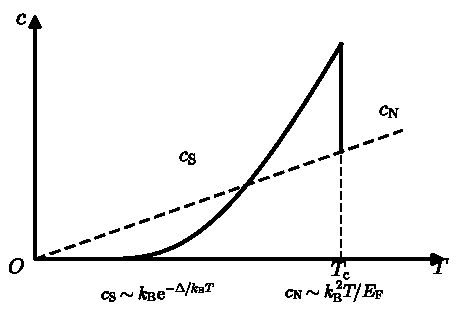
\includegraphics[width=6.5cm]{fig6-1.pdf}\\{\small 图 6.1\quad 超导体的电子比热容}
\end{minipage}
\end{center}

\begin{center}
\begin{minipage}{6cm}
\centering
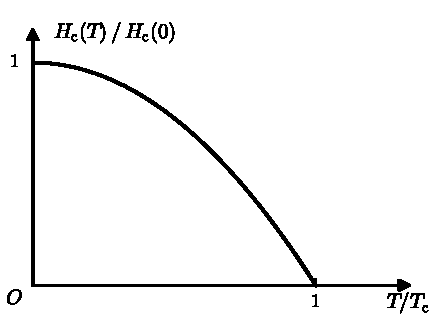
\includegraphics[width=6cm]{fig6-2.pdf}\\{\small 图 6.2\quad 超导体的临界磁场}
\end{minipage}
\end{center}

\subsection*{2. 存在能隙}

现在已有大量事实证明超导体中准粒子激发存在能隙，其中最有力的证据是隧道效应.若用很薄的氧化层（约2.5nm）将超导体（S）与正常金属（N）隔开，就在S与N之间形成了势垒.根据量子力学隧道效应理论，单电子可以穿透势垒，其隧穿电流I应与外加电压V成正比.但是，实验发现当 $T<T_{\mathrm{c}}$ 时，V必须大于 $(\Delta/e)$ 才有隧道电流，只有当 $T>T_{\mathrm{c}}$ 时才是直线，它们分别对应于图6.3中的实线与虚线.这一事实直接地证明了，从超导相中激发出一个准粒子至少要 $\Delta$ 能量，即存在能隙.超导体中的超声衰减与 $\exp(-\Delta/k_{\mathrm{B}}T)$ 成正比，同样表明有能隙.这些实验说明在费密面附近电子能谱发生了显著变化，不再是金属的费密球分布（因为在费密球面上有 $\delta E=0$ 的单粒子激发），费密球将改组.20世纪50年代初期人们做同位素实验又进一步发现，超导转变温度与晶格离子的同位素质量有 $T_{\mathrm{c}}M^{\alpha}=$ 常数的关系，其中 $\alpha$ 约等于1/2.这一发现说明超导转变与电子声子相互作用有关，其后的理论工作，都集中于从电子-声子相互作用证明能隙存在.

\begin{center}
\begin{minipage}{5cm}
\centering
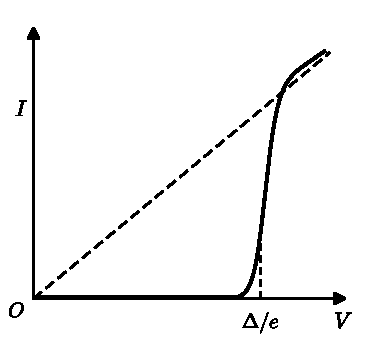
\includegraphics[width=5cm]{fig6-3.pdf}\\{\small 图 6.3\quad 隧道效应}
\end{minipage}
\end{center}

\subsection*{3. 迈斯纳效应}

迈斯纳效应指的是，在超导态弱磁场不能透入宏观样品内部，超导体对于弱场是完全逆磁体，这也是早期发现的超导特性.以后又发现对于超导合金，磁场可以透入超导体内部，但不破坏超导性，持续电流仍然存在，这类超导体称为第二类超导体，有迈斯纳效应的超导体则称为第一类超导体.对于第一类超导体，磁场超过 $H_{\mathrm{c}}(T)$ 以后，磁力线将透入样品内部，同时超导态也就被破坏，恢复为正常态.本章限于篇幅将着重于讨论第一类超导体.

对于大块纯金属样品只要证明了超导相的凝聚特性（凝聚能和能隙）就可以解释常规超导体的诸实验事实.巴丁（Bardeen）、库柏（Cooper）和施里弗（Schrieffer）（以后简称BCS）认为电子间通过交换虚声子所产生超导基态是，费密面附近相反动量及自旋的电子对通过吸引互作用形成了束缚电子对状态，称为库柏对组态.这一组态比正常费密球分布的能量要低 $g(0)\Delta^{2}$ 量级，这就是超导相的凝聚能.问题的新颖之处还在于，从这个基态的任何单粒子激发都要拆开库柏对，付出 $E_{k}=\sqrt{\varepsilon_{k}^{2}+\Delta^{2}}$ 的能量，其中 $\varepsilon_{k}$ 代表从费密能 $E_{\mathrm{F}}$ 算起的自由电子能量.因此，在费密面上激发一个准粒子至少要 $\Delta$ 能量，从而证明了能隙存在.由此出发可以解释常规超导体中的超导持续电流，迈斯纳效应和比热容的反常变化等一系列超导现象.我们将在本章中系统地介绍BCS超导理论及其对常规超导体的应用.习惯上，人们又将常规超导体称为BCS超导体.

\section{BCS约化哈密顿量}

现在分析电子交换虚声子的有效互作用
\begin{equation}
  H_{\mathrm{eff}}=\frac{1}{2}\sum_{\substack{q,\,k_{1},\,k_{2}\\\sigma_{1},\,\sigma_{2}}}
  V_{k_{1},q}\,C^{+}_{k_{1}+q,\,\sigma_{1}}C^{+}_{k_{2}-q,\,\sigma_{2}}
  C_{k_{2},\,\sigma_{2}}C_{k_{1},\,\sigma_{1}}
\end{equation}
根据式(5.5.21)其中互作用系数为
\begin{equation}
  V_{k_{1},q}=|D_{q}|^{2}
  \frac{2\hbar\omega_{q}}{(E_{k_{1}+q}-E_{k_{1}})^{2}-(\hbar\omega_{q})^{2}}
\end{equation}
在费密面附近 $|E_{k_{1}+q}-E_{k_{1}}|<\hbar\omega_{q}\approx\hbar\omega_{\mathrm{D}}$ 能壳内 $V_{k_{1},q}<0$，$H_{\mathrm{eff}}$ 为吸引互作用，在能壳外 $V_{k_{1},q}>0$，为排斥互作用，这里 $\omega_{\mathrm{D}}$ 为声子的德拜频率，$\hbar\omega_{\mathrm{D}}\sim10^{-2}$ eV.由于声学模声子的最大态密度在 $\omega_{\mathrm{D}}$ 附近，人们可以将式(6.2.2)中厚度随 $\omega_{q}$ 变化的吸引区近似用费密面附近厚度为 $2\hbar\omega_{\mathrm{D}}$ 的固定能壳区代替，这是一种合理的简化.此外，金属中电子还存在直接库仑作用，可以用屏蔽库仑势表示
\begin{equation}
  H_{\mathrm{coul}}=\frac{1}{2}\sum_{\substack{q,\,k_{1},\,k_{2}\\\sigma_{1},\,\sigma_{2}}}
  \frac{4\pi e^{2}}{q^{2}+\lambda^{2}}C^{+}_{k_{1}+q,\,\sigma_{1}}C^{+}_{k_{2}-q,\,\sigma_{2}}
  C_{k_{2},\,\sigma_{2}}C_{k_{1},\,\sigma_{1}}
\end{equation}
$H_{\mathrm{coul}}$ 是电子间的排斥势.如果电子与声子的耦合常数适当大，则在费密面附近 $2\hbar\omega_{\mathrm{D}}$ 能壳内吸引势 $V_{k_{1},q}$ 可以超过屏蔽库仑势 $\dfrac{4\pi e^{2}}{q^{2}+\lambda^{2}}$，从而产生电子之间的净吸引互作用，这是产生超导凝聚的原因.

巴丁等人认为在 $2\hbar\omega_{\mathrm{D}}$ 能壳外的排斥相互作用可以略去，而能壳内的净吸引互作用 $(V_{k_{1},q}+\frac{4\pi e^{2}}{q^{2}+\lambda^{2}})$ 可近似用常数代替，这时电子之间的相互作用写成下列简化形式
\begin{equation}
  H'=-\frac{1}{2}V\sum_{\substack{q,\,k_{1},\,k_{2}\\\sigma_{1},\,\sigma_{2}}}
  C^{+}_{k_{1}+q,\,\sigma_{1}}C^{+}_{k_{2}-q,\,\sigma_{2}}
  C_{k_{2},\,\sigma_{2}}C_{k_{1},\,\sigma_{1}}
\end{equation}
其中V为正量，而且仅在 $|E_{k_{1}+q}-E_{k_{1}}|<\hbar\omega_{\mathrm{D}}$ 区内 $V\neq0$.物理上，BCS的这一简化就是，在讨论电子间的净吸引互作用时，假定它与取向无关，相当于取各向同性的s波散射近似.在§4中我们将看到，正是此假定导致超导配对的能隙与电子间的相对取向无关，使声子机制的BCS超导体成为各向同性配对的超导体.

根据式(6.2.4)，一对电子 $(\boldsymbol{k}_{1},\sigma_{1})$ 和 $(\boldsymbol{k}_{2},\sigma_{2})$ 散射后变为 $(\boldsymbol{k}_{1}+\boldsymbol{q},\sigma_{1})$ 和 $(\boldsymbol{k}_{2}-\boldsymbol{q},\sigma_{2})$，总波矢守恒，令
\begin{equation*}
  \boldsymbol{K}=\boldsymbol{k}_{1}+\boldsymbol{k}_{2}
\end{equation*}
将 $\boldsymbol{H}'$ 改写为
\begin{equation*}
  H'=-\frac{V}{2}\sum_{\substack{q,\,k_{1},\,k_{2}\\\sigma_{1},\,\sigma_{2}}}
  C^{+}_{k_{1}+q,\,\sigma_{1}}C^{+}_{K-k_{1}-q,\,\sigma_{2}}
  C_{K-k_{1},\,\sigma_{2}}C_{k_{1},\,\sigma_{1}}
\end{equation*}
再设 $\boldsymbol{k}'=\boldsymbol{k}+\boldsymbol{q}$，$\boldsymbol{k}=\boldsymbol{k}_{1}$，$\sigma_{1}=\sigma$，$\sigma_{2}=\sigma'$，则 $\boldsymbol{H}'$ 可按总波矢K分类
\begin{equation}
  H'=\sum_{K}H'_{K}
\end{equation}
其中
\begin{equation}
  H'_{K}\equiv-\frac{V}{2}\sum_{k,\,k',\,\sigma,\,\sigma'}
  C^{+}_{k',\,\sigma}C^{+}_{K-k',\,\sigma'}C_{K-k,\,\sigma'}C_{k,\,\sigma}
\end{equation}
代表系统中总波矢为K的电子对间相互作用.对于不同的K，具有吸引互作用的电子对数目不同，由图6.4中阴影区绕K轴转成的体积决定.显然，$\boldsymbol{K}\neq0$ 时，这个体积随K值变化不大.但是，$\boldsymbol{K}=0$ 情况十分特殊，这时电子对吸引区就是能量差为 $2\hbar\omega_{\mathrm{D}}$ 的两同心球间体积，它大于任一个"$\boldsymbol{K}\neq0$ 对"的相体积.因此 $\boldsymbol{K}=0$ 电子对占有最大相体积.换句话说，$H'_{K=0}$ 的散射互作用比 $H'_{K\neq0}$ 占更大优势，可以略去式(6.2.5)中 $\boldsymbol{K}\neq0$ 项，只取K=0电子对项
\begin{equation}
  H'=-\frac{V}{2}\sum_{k,\,k',\,\sigma,\,\sigma'}
  C^{+}_{k',\,\sigma}C^{+}_{-k',\,\sigma'}C_{-k,\,\sigma'}C_{k,\,\sigma}
\end{equation}
式(6.2.7)代表准动量相反的电子对的吸引互作用，其中 $\sigma'$ 可取 $\pm\sigma$ 两种状态，正号对应于两电子自旋平行，负号为反平行取向.由于泡利不相容原理将限制自旋平行电子在位置空间靠拢，因此式(6.2.7)中 $\sigma'=\sigma$ 项的贡献比 $\sigma'=-\sigma$ 项小，也可略去，最后将互作用取为
\begin{equation}
  H'=-\frac{V}{2}\sum_{k,\,k',\,\sigma}
  C^{+}_{k',\,\sigma}C^{+}_{-k',\,-\sigma}C_{-k,\,-\sigma}C_{k,\,\sigma}
\end{equation}

\begin{center}
\begin{minipage}{6cm}
\centering
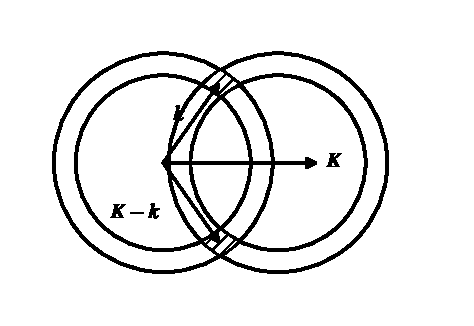
\includegraphics[width=6cm]{fig6-4.pdf}\\{\small 图 6.4\quad 总波矢为K时电子对的吸引区（阴影区）}
\end{minipage}
\end{center}

加上电子能量即为总哈密顿量
\begin{equation*}
\begin{aligned}
  \hat{H}&=\sum_{k,\,\sigma}E_{k}C^{+}_{k,\,\sigma}C_{k,\,\sigma}
  -\frac{V}{2}\sum_{k,\,k',\,\sigma}
  C^{+}_{k',\,\sigma}C^{+}_{-k',\,-\sigma}C_{-k,\,-\sigma}C_{k,\,\sigma}\\
  &=\sum_{k}E_{k}\left(C^{+}_{k\uparrow}C_{k\uparrow}
  +C^{+}_{k\downarrow}C_{k\downarrow}\right)\\
  &\quad-\frac{V}{2}\sum_{k,\,k'}\left(C^{+}_{k'\uparrow}C^{+}_{-k'\downarrow}
  C_{-k\downarrow}C_{k\uparrow}
  +C^{+}_{k'\downarrow}C^{+}_{-k'\uparrow}C_{-k\uparrow}C_{k\downarrow}\right)
\end{aligned}
\end{equation*}
对上式右边最后一项作代换 $(k,k')\to(-k,-k')$ 并考虑到 $E_{-k}=E_{k}$，整理后得
\begin{equation}
  \hat{H}=\sum_{k}E_{k}\left(C^{+}_{k\uparrow}C_{k\uparrow}
  +C^{+}_{-k\downarrow}C_{-k\downarrow}\right)
  -V\sum_{k,\,k'}C^{+}_{k'\uparrow}C^{+}_{-k'\downarrow}C_{-k\downarrow}C_{k\uparrow}
\end{equation}
这就是BCS理论用于描述超导基态的哈密顿量，其基本假定是，在费密面附近准动量和自旋都相反的电子之间的吸引互作用是产生超导凝聚的主要原因.由于式(6.2.9)中 $(k,\uparrow)$ 或 $(-k,\downarrow)$ 总是同时出现，可采用简化记号，令k代表 $(k,\uparrow)$，$-k$ 代表 $(-k,\downarrow)$，则BCS的哈密顿量简化为
\begin{equation}
  \hat{H}=\sum_{k}E_{k}\left(C^{+}_{k}C_{k}+C^{+}_{-k}C_{-k}\right)
  -V\sum_{k,\,k'}C^{+}_{k'}C^{+}_{-k'}C_{-k}C_{k}
\end{equation}
在以后的讨论中，将从下列约化哈密顿量出发：
\begin{equation}
  \overline{H}=\hat{H}-E_{\mathrm{F}}\hat{N}
  =\sum_{k}\varepsilon_{k}\left(C^{+}_{k}C_{k}+C^{+}_{-k}C_{-k}\right)
  -V\sum_{k,\,k'}C^{+}_{k'}C^{+}_{-k'}C_{-k}C_{k}
\end{equation}
其中
\begin{equation}
  \varepsilon_{k}=E_{k}-E_{\mathrm{F}}
\end{equation}
代表从费密面算起的自由电子能量，吸引互作用V仅在 $|\varepsilon_{k}|<\hbar\omega_{\mathrm{D}}$ 区域内不等于零.约化哈密顿量选用 $\overline{H}$ 的理由是因为在超导问题中总粒子数不守恒（详见§9），所以取 $\overline{H}=\hat{H}-E_{\mathrm{F}}\hat{N}$，相当于用热力学势代替自由能讨论粒子数可变系统.

\section{库柏对}

为了研究费密面附近吸引互作用对系统的电子状态和能量将产生什么影响，库柏\textsuperscript{[1]}讨论了 $T=0$ K时在已被填满的费密球外附加两个电子的相互作用问题.为使问题简化，库柏假设费密球内电子可当自由电子处理.因此，费密球的存在仅起着禁止附加电子占据 $k<k_{\mathrm{F}}$ 状态的作用，可以完全忽略费密球内电子被散射到球外的复杂情况，只考虑附加电子之间的相互作用.这样，只需处理二体散射问题.

设这两个附加电子具有相反的动量和自旋，其状态由 $C^{+}_{k}C^{+}_{-k}|F\rangle$ 描述，$|F\rangle$ 代表费密球被填满的正常电子基态.但是状态 $C^{+}_{k}C^{+}_{-k}|F\rangle$ 并非哈密顿量
\begin{equation*}
  \overline{H}=\sum_{k}\varepsilon_{k}\left(C^{+}_{k}C_{k}+C^{+}_{-k}C_{-k}\right)
  -V\sum_{k,\,k'>k_{\mathrm{F}}}C^{+}_{k'}C^{+}_{-k'}C_{-k}C_{k}
\end{equation*}
的本征函数，因为互作用将导致 $(\boldsymbol{k},-\boldsymbol{k})$ 散射为 $(\boldsymbol{k}',-\boldsymbol{k}')$，使状态变为 $C^{+}_{k'}C^{+}_{-k'}|F\rangle$.根据叠加原理，$\overline{H}$ 的本征态应当包括所有可能散射状态的线性组合，即
\begin{equation}
  |\psi\rangle=\sum_{k>k_{\mathrm{F}}}a(k)C^{+}_{k}C^{+}_{-k}|F\rangle
\end{equation}
其中求和k限于费密球外吸引区 $0<\varepsilon_{k}<\hbar\omega_{\mathrm{D}}$，$a(k)$ 为待定系数.从 $\overline{H}$ 的本征值可求得费密球外两个附加电子的能量为
\begin{equation}
  E=2\sum_{k>k_{\mathrm{F}}}\varepsilon_{k}|a(k)|^{2}
  -V\sum_{k,\,k'>k_{\mathrm{F}}}a^{*}(k')a(k)
\end{equation}
$a(k)$ 由E的变分极值决定.由于 $|\psi\rangle$ 是归一的，还存在变分条件 $\langle\psi|\psi\rangle=\sum_{k}|a(k)|^{2}=1$，我们必须引进拉氏乘子 $\lambda$ 求 $\left\{E-\lambda\sum_{k}|a(k)|^{2}\right\}$ 的极值，得到 $a(k)$ 的极值方程
\begin{equation}
  \left(2\varepsilon_{k}-\lambda\right)a(k)=V\sum_{k'>k_{\mathrm{F}}}a(k')
\end{equation}
此方程可直接求解，定出λ.令
\begin{equation}
  \sum_{k>k_{\mathrm{F}}}a(k)\equiv A
\end{equation}
代入方程(6.3.3)得到
\begin{equation}
  a(k)=\frac{V}{2\varepsilon_{k}-\lambda}
\end{equation}
再对k求和并利用(6.3.4)，则对于A的非零解满足下列自洽方程：
\begin{equation}
  1=V\sum_{k>k_{\mathrm{F}}}\frac{1}{2\varepsilon_{k}-\lambda}
  \qquad(0<\varepsilon_{k}<\hbar\omega_{\mathrm{D}})
\end{equation}
对于吸引互作用 $V>0$，上式存在一个 $\lambda$ 为负值的解，为求出此解，可将求和换为积分
\begin{equation}
  \sum_{k>k_{\mathrm{F}}}\frac{1}{2\varepsilon_{k}-\lambda}
  =\int_{0}^{\hbar\omega_{\mathrm{D}}}\mathrm{d}\varepsilon\,
  \frac{g(\varepsilon)}{2\varepsilon-\lambda}
\end{equation}
考虑到积分区域较窄，可近似用费密面上某自旋取向的态密度 $g(0)$ 代替积分中 $g(\varepsilon)$，于是式(6.3.6)写为
\begin{equation}
  1=g(0)V\int_{0}^{\hbar\omega_{\mathrm{D}}}\frac{\mathrm{d}\varepsilon}{2\varepsilon-\lambda}
\end{equation}
积分后求得
\begin{equation}
  \lambda=\frac{-2\hbar\omega_{\mathrm{D}}}
  {\exp\Bigl[\dfrac{2}{g(0)V}\Bigr]-1}
\end{equation}
将式(6.3.5)两边乘以 $a^{*}(k)$ 并对k求和，再利用式(6.3.2)和归一条件 $\sum_{k}|a(k)|^{2}=1$，可证明
\begin{equation}
  \lambda=2\sum_{k}\varepsilon_{k}|a(k)|^{2}
  -V\sum_{k,\,k'}a^{*}(k)a(k')=E
\end{equation}
根据式(6.3.9)，当 $g(0)V\ll1$ 时
\begin{equation}
  E=-2\hbar\omega_{\mathrm{D}}\exp\Bigl[-\frac{2}{g(0)V}\Bigr]<0
\end{equation}
E代表弱吸引互作用情况下，两个电子互作用系统的能量最小值.$E<0$ 说明形成了电子对的束缚态，称为库柏对，库柏对中两个电子的动量和自旋取向都相反，由此可得下列重要结论：

（i）费密球外一对动量和自旋相反的电子之间只要存在净的吸引互作用，不管它多弱，都能形成束缚电子对.

（ii）由于E从费密面算起，因此 $E<0$ 表示费密球外附加电子对形成束缚态的能量比费密面上一对自由电子的能量还低.这表明存在吸引互作用时费密球不再是稳定的分布，电子将由于形成库柏对获得能量.超导基态应由库柏对组成，而不再是正常的电子费密球分布.

（iii）由于|E|代表库柏对的结合能，因此拆散库柏对需要 $2\hbar\omega_{\mathrm{D}}\exp\Bigl[-\dfrac{2}{g(0)V}\Bigr]$ 的能量.此外由于 $\exp\Bigl[-\dfrac{2}{g(0)V}\Bigr]$ 因子的存在，当 $V\to0$ 时库柏对的结合能不能展开为V的幂级数，说明库柏问题不能用微扰论求解，相应的超导理论也必须建立在非微扰计算的基础上.

（iv）库柏对的尺寸：利用不确定关系，可以估计电子对的尺寸.设库柏对的半径为 $\rho_{\mathrm{c}}$，局限于这个尺度的电子有动量不确定度 $\delta p\sim\hbar/\rho_{\mathrm{c}}$，相应的动能不确定度 $v_{\mathrm{F}}\delta p$ 应小于库柏对的结合能 $|E|=2\hbar\omega_{\mathrm{D}}\exp\Bigl[-\dfrac{2}{g(0)V}\Bigr]$.因此，$\delta p\sim\dfrac{|E|}{v_{\mathrm{F}}}$，这里 $v_{\mathrm{F}}$ 为费密速度，于是
\begin{equation}
  \rho_{\mathrm{c}}\sim\frac{\hbar}{\delta p}\sim\frac{\hbar v_{\mathrm{F}}}{|E|}
  \sim\frac{E_{\mathrm{F}}}{k_{\mathrm{F}}|E|}
\end{equation}
由于 $E_{\mathrm{F}}$ 为电子伏量级，$k_{\mathrm{F}}\sim10^{8}\,\mathrm{cm}^{-1}$，而|E|可根据超导转变温度（$T_{\mathrm{c}}<10$ K）估计，|E|约为 $10^{-4}$ eV量级，因此库柏对的尺寸 $\rho_{\mathrm{c}}\sim10^{-4}$ cm，它大约是晶格常数的一万倍.换句话说，在库柏对尺度内，必然存在着许多电子对，它们的运动是相互关联的.这样，为了正确解释超导电性，人们必须计及所有电子之间的相互作用，超导问题将是一个真正的多体问题.

对于超导体，人们还定义一个重要参量 $\xi_{0}$ 描述电子运动相互关联的空间尺寸，称为相干长度.相干长度 $\xi_{0}$ 大致为库柏对的尺寸 $\rho_{\mathrm{c}}$.在BCS超导理论中相干长度取为
\begin{equation}
  \xi_{0}=\frac{\hbar v_{\mathrm{F}}}{\pi\Delta(0)}
\end{equation}
$\Delta(0)$ 是超导体的零温能隙，代表激发一个准粒子所需最小能量.在超导体中，只有当电子的动能不确定度小于 $\Delta(0)$ 时，电子才可能结合成库柏对.因此，多体理论中电子对的尺寸由式(6.3.13)估计，因子 $\dfrac{1}{\pi}$ 是为了以后讨论方便所加入的.相干长度 $\xi_{0}$ 对超导体的电磁性能有重要影响，具体情况将在§7与§8中介绍.

\section{\texorpdfstring{BCS超导理论\textsuperscript{[2]}}{BCS超导理论[2]}}

由于库柏证明了吸引互作用使费密球改组，形成k与$-k$电子的束缚态，因此巴丁、库柏等人设想超导基态是电子按照库柏对分布的状态.他们认为，由于费密球改组，在k空间中任一对状态k与$(-k)$（即k，↑态与$-k$，↓态）的占据情况均应当由变分极值条件确定.设 $v_{k}$ 是对状态被占据的概率幅，$u_{k}$ 代表对状态未被占据的概率幅，则BCS超导基态的变分试探函数写为
\begin{equation}
  |0\rangle=\prod_{k}\left(u_{k}+v_{k}C^{+}_{k}C^{+}_{-k}\right)|\mathrm{Vac}\rangle
\end{equation}
其中 $|\mathrm{Vac}\rangle$ 是真正的真空状态 $\left(C_{k}|\mathrm{Vac}\rangle=0\right)$.由于 $u_{k}^{2}$ 与 $v_{k}^{2}$ 代表对状态未被占据和被占据的概率，应满足归一条件 $u_{k}^{2}+v_{k}^{2}=1$.人们可以用变分法同时决定超导基态能量 $\langle0|\overline{H}|0\rangle$ 及系数 $u_{k}$ 和 $v_{k}$，这是巴丁等人原来的做法.为简单起见，我们将采用自洽场近似法，其实质与BCS变分法相同，但便于推广到 $T>0$ 和空间非均匀等情形.

为了求出 $\overline{H}=\hat{H}-E_{\mathrm{F}}\hat{N}$ 的本征函数和本征值，我们先将约化哈密顿量式(6.2.11)用算符的二次型近似表示，然后利用玻戈留玻夫变换使它对角化.

根据库柏对组成超导基态的想法，可假定下列对算符的基态平均值存在，且不等于零
\begin{equation}
  \left.
  \begin{aligned}
    &\langle C^{+}_{k}C^{+}_{-k}\rangle\equiv
    \langle0|C^{+}_{k}C^{+}_{-k}|0\rangle\neq0\\
    &\langle C_{-k}C_{k}\rangle\equiv
    \langle0|C_{-k}C_{k}|0\rangle\neq0
  \end{aligned}\right\}
\end{equation}
将对算符写成
\begin{equation}
  \left.
  \begin{aligned}
    &C_{-k}C_{k}=\langle C_{-k}C_{k}\rangle
    +\left(C_{-k}C_{k}-\langle C_{-k}C_{k}\rangle\right)\\
    &C^{+}_{k}C^{+}_{-k}=\langle C^{+}_{k}C^{+}_{-k}\rangle
    +\left(C^{+}_{k}C^{+}_{-k}-\langle C^{+}_{k}C^{+}_{-k}\rangle\right)
  \end{aligned}\right\}
\end{equation}
取近似方案：设电子对算符与其平均值之差为小量，代入BCS的互作用项 $\left\{-V\sum_{k,k'}C^{+}_{k'}C^{+}_{-k'}C_{-k}C_{k}\right\}$ 中，取一阶近似，求得下列二次型哈密顿量
\begin{equation}
\begin{aligned}
  \overline{H}&\approx\sum_{k}\varepsilon_{k}
  \left(C^{+}_{k}C_{k}+C^{+}_{-k}C_{-k}\right)
  -V\sum_{k,\,k'}\left\{C^{+}_{k'}C^{+}_{-k'}\langle C_{-k}C_{k}\rangle\right.\\
  &\quad\left.+C_{-k}C_{k}\langle C^{+}_{k'}C^{+}_{-k'}\rangle
  -\langle C^{+}_{k'}C^{+}_{-k'}\rangle\langle C_{-k}C_{k}\rangle\right\}
\end{aligned}
\end{equation}
称为自洽场近似（self-consistent field approximation，SCFA）的哈密顿量.SCFA实际上是一种改进的平均场近似（MFA），它将 $\overline{H}$ 中"对算子" $C_{-k}C_{k}$ 用其平均量 $\langle C_{-k}C_{k}\rangle$ 代替，其中 $\langle\cdots\rangle$ 是对超导基态的对角平均.由于超导基态 $|0\rangle$ 尚属未知，因此式(6.4.4)中 $\langle C_{-k}C_{k}\rangle$ 等平均量也是未知的，必须在上述MFA方案下求出近似的基态解之后，才能自洽确定 $\langle C_{-k}C_{k}\rangle$ 等平均量，正因此，上述近似被称为自洽场近似.再定义
\begin{equation}
  \Delta=V\sum_{k}\langle C_{-k}C_{k}\rangle\text{，}
  \qquad \Delta^{*}=V\sum_{k}\langle C^{+}_{k}C^{+}_{-k}\rangle
\end{equation}
这里 $\Delta$ 与 $\Delta^{*}$ 只在吸引区（$V\neq0$）中不为零.在一般情况下，$\Delta$ 为复量，对于孤立的均匀大块样品系统，可取为 $\Delta=|\Delta|\mathrm{e}^{\mathrm{i}\varphi}$ 及 $\Delta^{*}=|\Delta|\mathrm{e}^{-\mathrm{i}\varphi}$，其中相位 $\varphi$ 为任意常数.为了简化计算，可以取特定值 $\varphi=0$，则有 $\Delta=\Delta^{*}=|\Delta|$ 为实量，相当于略去相位因子，这时 $\Delta^{2}=|\Delta|^{2}=\Delta^{*}\Delta$.但是，在空间非均匀情况下，当涉及两块超导体的连接系统时，相位因子 $\mathrm{e}^{\mathrm{i}\varphi}$ 不能略去，我们将在§9和§10中作进一步的说明.现在，为简单起见，仅考虑 $\Delta$ 为实量，取 $\Delta^{2}=\Delta^{*}\Delta$ 并将式(6.4.4)写成
\begin{equation}
  \overline{H}\approx\sum_{k}\varepsilon_{k}
  \left(C^{+}_{k}C_{k}+C^{+}_{-k}C_{-k}\right)
  -\Delta\sum_{k}\left(C^{+}_{k}C^{+}_{-k}+C_{-k}C_{k}\right)+\Delta^{2}/V
\end{equation}
由于上式中的 $\Delta$ 相当于"对算子" $\left(C^{+}_{k}C^{+}_{-k}+C_{-k}C_{k}\right)$ 的外势场，所以 $\Delta$ 又称为对势.这是一个简单的二次型，属于严格可解的模型，我们将利用玻戈留玻夫的正则变换方法将式(6.4.6)对角化.

考查运动方程
\begin{equation}
  \mathrm{i}\dot{C}_{k}=\left[C_{k},\overline{H}\right]
  =\varepsilon_{k}C_{k}-\Delta C^{+}_{-k}
\end{equation}
\begin{equation}
  \mathrm{i}\dot{C}_{-k}=\left[C_{-k},\overline{H}\right]
  =\varepsilon_{k}C_{-k}+\Delta C^{+}_{k}
\end{equation}
可知 $C_{k}$ 与 $C^{+}_{-k}$ 相耦合，而 $C_{-k}$ 则与 $C^{+}_{k}$ 耦合.为使 $\overline{H}$ 对角化求得其本征值，应组合 $C_{k}$ 与 $C^{+}_{-k}$ 引入新算符 $\alpha_{k}$，而 $\alpha_{-k}$ 则由 $C_{-k}$ 与 $C^{+}_{k}$ 构成，即作下列实系数正则变换：
\begin{equation}
  \left.
  \begin{aligned}
    &\alpha_{k}=u_{k}C_{k}-v_{k}C^{+}_{-k}\text{，}
    \qquad \alpha^{+}_{k}=u_{k}C^{+}_{k}-v_{k}C_{-k}\\
    &\alpha_{-k}=u_{k}C_{-k}+v_{k}C^{+}_{k}\text{，}
    \qquad \alpha^{+}_{-k}=u_{k}C^{+}_{-k}+v_{k}C_{k}
  \end{aligned}\right\}
\end{equation}
要求新算符同样满足费密子的对易律
\begin{equation}
\begin{aligned}
  \left[\alpha_{k},\alpha^{+}_{k'}\right]_{+}
  &=u_{k}u_{k'}\left[C_{k},C^{+}_{k'}\right]_{+}
  +v_{k}v_{k'}\left[C^{+}_{-k},C_{-k'}\right]_{+}\\
  &=\delta_{kk'}\left(u_{k}^{2}+v_{k}^{2}\right)=\delta_{kk'}
\end{aligned}
\end{equation}
和
\begin{equation}
\begin{aligned}
  \left[\alpha_{k},\alpha_{-k'}\right]_{+}
  &=u_{k}v_{k'}\left[C_{k},C^{+}_{k'}\right]_{+}
  -v_{k}u_{k'}\left[C^{+}_{-k},C_{-k'}\right]_{+}\\
  &=\delta_{kk'}\left(u_{k}v_{k}-u_{k}v_{k}\right)=0
\end{aligned}
\end{equation}
类似，有
\begin{equation}
  \left[\alpha_{-k},\alpha^{+}_{-k'}\right]_{+}
  =\delta_{kk'}\left(u_{k}^{2}+v_{k}^{2}\right)=\delta_{kk'}
\end{equation}
\begin{equation}
  \left[\alpha^{+}_{k},\alpha^{+}_{-k'}\right]_{+}=0
\end{equation}
从式(6.4.10)与式(6.4.12)得到 $u_{k}$ 与 $v_{k}$ 的一个关系式
\begin{equation}
  u_{k}^{2}+v_{k}^{2}=1
\end{equation}
而玻戈留玻夫基本变换式(6.4.9)写成
\begin{equation}
  \left.
  \begin{aligned}
    &C_{k}=u_{k}\alpha_{k}+v_{k}\alpha^{+}_{-k}\text{，}
    \qquad C^{+}_{k}=u_{k}\alpha^{+}_{k}+v_{k}\alpha_{-k}\\
    &C_{-k}=u_{k}\alpha_{-k}-v_{k}\alpha^{+}_{k}\text{，}
    \qquad C^{+}_{-k}=u_{k}\alpha^{+}_{-k}-v_{k}\alpha_{k}
  \end{aligned}\right\}
\end{equation}
将上式代入 $\overline{H}$ 的近似式(6.4.6)中，经整理后
\begin{equation}
\begin{aligned}
  \overline{H}&=\sum_{k}\bigl\{\bigl[\varepsilon_{k}(u_{k}^{2}-v_{k}^{2})
  +2\Delta u_{k}v_{k}\bigr]\left(\alpha^{+}_{k}\alpha_{k}
  +\alpha^{+}_{-k}\alpha_{-k}\right)\\
  &\quad+\bigl[2\varepsilon_{k}u_{k}v_{k}
  -\Delta\left(u_{k}^{2}-v_{k}^{2}\right)\bigr]
  \left(\alpha^{+}_{k}\alpha^{+}_{-k}
  +\alpha_{-k}\alpha_{k}\right)\bigr\}\\
  &\quad+\sum_{k}\left[2\varepsilon_{k}v_{k}^{2}-2u_{k}v_{k}\Delta\right]
  +\frac{\Delta^{2}}{V}
\end{aligned}
\end{equation}
再要求非对角项 $\left(\alpha^{+}_{k}\alpha^{+}_{-k}
+\alpha_{-k}\alpha_{k}\right)$ 的系数等于零，求得 $u_{k}$ 与 $v_{k}$ 的另一个关系式
\begin{equation}
  \Delta\left(u_{k}^{2}-v_{k}^{2}\right)=2\varepsilon_{k}u_{k}v_{k}
\end{equation}
上式又称对角化条件，它与式(6.4.14)联立并消去 $v_{k}$，得方程
\begin{equation}
  \left(u_{k}^{2}\right)^{2}-\left(u_{k}^{2}\right)
  +\frac{1}{4}\frac{\Delta^{2}}{\xi_{k}^{2}}=0
\end{equation}
其中
\begin{equation}
  \xi_{k}=\sqrt{\varepsilon_{k}^{2}+\Delta^{2}}
  \qquad\left(\varepsilon_{k}=E_{k}-E_{\mathrm{F}}\right)
\end{equation}
式(6.4.18)的解为 $u_{k}^{2}=\frac{1}{2}\left(1\pm\frac{\varepsilon_{k}}{\xi_{k}}\right)$，$v_{k}^{2}=1-u_{k}^{2}=\frac{1}{2}\left(1\mp\frac{\varepsilon_{k}}{\xi_{k}}\right)$. $u_{k}^{2}$ 与 $v_{k}^{2}$ 的选择应参考正常态（$\Delta=0$ 时）的费密分布.显然，应取
\begin{equation}
  u_{k}^{2}=\frac{1}{2}\left(1+\frac{\varepsilon_{k}}{\xi_{k}}\right)\text{，}\qquad
  v_{k}^{2}=\frac{1}{2}\left(1-\frac{\varepsilon_{k}}{\xi_{k}}\right)
\end{equation}
这是因为当 $\Delta=0$ 时，$\xi_{k}=|\varepsilon_{k}|$
\begin{equation}
\begin{aligned}
  u_{k}^{2}&=\frac{1}{2}\left(1+\frac{\varepsilon_{k}}{|\varepsilon_{k}|}\right)
  =\begin{cases}1&(k>k_{\mathrm{F}})\\0&(k<k_{\mathrm{F}})\end{cases}\\
  v_{k}^{2}&=\frac{1}{2}\left(1-\frac{\varepsilon_{k}}{|\varepsilon_{k}|}\right)
  =\begin{cases}0&(k>k_{\mathrm{F}})\\1&(k<k_{\mathrm{F}})\end{cases}
\end{aligned}
\end{equation}
此即费密球分布，这时
\begin{equation*}
  \alpha^{+}_{k}=u_{k}C^{+}_{k}-v_{k}C_{-k}
  =\begin{cases}
    C^{+}_{k} & (k>k_{\mathrm{F}})\text{，费密球外产生电子}\\
    C_{-k} & (k<k_{\mathrm{F}})\text{，费密球内产生空穴}
  \end{cases}
\end{equation*}
\begin{equation*}
  \alpha_{k}=u_{k}C_{k}-v_{k}C^{+}_{-k}
  =\begin{cases}
    C_{k} & (k>k_{\mathrm{F}})\text{，费密球外消灭电子}\\
    C^{+}_{-k} & (k<k_{\mathrm{F}})\text{，费密球内消灭空穴}
  \end{cases}
\end{equation*}
这样新算符 $\alpha_{k}$，$\alpha^{+}_{k}$ 自动演化为以费密面作分界的电子和空穴算符，说明 $\alpha_{k}$ 与 $\alpha^{+}_{k}$ 也可作为描述正常态电子与空穴激发的统一准粒子算符.

当 $\Delta\neq0$ 时，$u_{k}$ 与 $v_{k}$ 在费密球内和球外同时出现，这时 $\alpha_{k}$ 代表电子与空穴的某种混合.在物理上是因为有效吸引破坏了费密球分布，以致 $T=0$ K时不仅在 $k<k_{\mathrm{F}}$ 区域能产生空穴，$k>k_{\mathrm{F}}$ 区也能产生空穴（相应的 $k>k_{\mathrm{F}}$ 区能产生电子，$k<k_{\mathrm{F}}$ 区也能产生电子），如图6.6中实线所示.因此，玻戈留玻夫变换可理解为电子与空穴的混合.

将式(6.4.19)与(6.4.20)代入式(6.4.16)，并注意到
\begin{equation}
  \varepsilon_{k}\left(u_{k}^{2}-v_{k}^{2}\right)+2\Delta u_{k}v_{k}
  =\sqrt{\varepsilon_{k}^{2}+\Delta^{2}}=\xi_{k}
\end{equation}
求得对角化的哈密顿量
\begin{equation}
  \overline{H}=E_{\mathrm{s}}(0)+\sum_{k}\sqrt{\varepsilon_{k}^{2}+\Delta^{2}}
  \left(\alpha^{+}_{k}\alpha_{k}+\alpha^{+}_{-k}\alpha_{-k}\right)
\end{equation}
其中基态能量
\begin{equation}
  E_{\mathrm{s}}(0)=2\sum_{k}\varepsilon_{k}v_{k}^{2}
  -2\Delta\sum_{k}u_{k}v_{k}+\frac{\Delta^{2}}{V}
\end{equation}
而
\begin{equation*}
  \xi_{k}=\sqrt{\varepsilon_{k}^{2}+\Delta^{2}}
\end{equation*}
代表超导的元激发能量（或准粒子能量），$\alpha_{k}$ 为元激发算子.显然，当 $k\to k_{\mathrm{F}}$ 时，$\varepsilon_{k}\to0$，$\xi_{\mathrm{F}}=\Delta$，说明从费密面激发一个准粒子至少需要 $\Delta$ 能量，它代表元激发的能隙，这是正常金属所不具有的特征.图6.5表示 $\xi_{k}$ 与 $\varepsilon_{k}$ 及 $\Delta$ 的关系.

\begin{center}
\begin{minipage}{7cm}
\centering
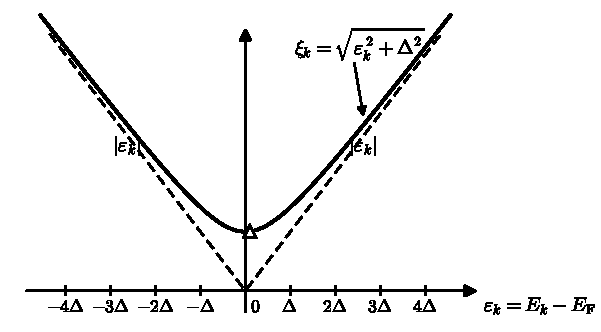
\includegraphics[width=7cm]{fig6-5.pdf}\\{\small 图 6.5\quad 超导体的元激发}
\end{minipage}
\end{center}

下面分别讨论超导能隙，凝聚能，基态和超电流等问题.

\subsection*{1. 能隙$\Delta$的计算}

$T=0$ K时的 $\Delta$，可通过元激发算子 $\alpha_{k}$ 对基态的自洽平均来确定.由于此时无准粒子激发，并且准粒子算符的非对角平均 $\langle\alpha_{-k}\alpha_{k}\rangle=\langle\alpha^{+}_{k}\alpha^{+}_{-k}\rangle=0$，将得到
\begin{equation}
\begin{aligned}
  \Delta&\equiv V\sum_{k}\langle C_{-k}C_{k}\rangle\\
  &=V\sum_{k}\langle0|\left(u_{k}\alpha_{-k}-v_{k}\alpha^{+}_{k}\right)
  \left(u_{k}\alpha_{k}+v_{k}\alpha^{+}_{-k}\right)|0\rangle\\
  &=V\sum_{k}u_{k}v_{k}
\end{aligned}
\end{equation}
利用式(6.4.17)和式(6.4.20)，将上式改写为
\begin{equation}
  \Delta=\frac{1}{2}V\sum_{k}\frac{\Delta}{\xi_{k}}
\end{equation}
当 $\Delta\neq0$ 时，从上式得能隙方程
\begin{equation}
  1=\frac{1}{2}V\sum_{k}\frac{1}{\sqrt{\varepsilon_{k}^{2}+\Delta^{2}}}
\end{equation}
将求和化为积分，并用费密面上一种自旋取向的态密度 $g(0)$ 近似表示吸引区内 $\left(|\varepsilon_{k}|\leqslant\hbar\omega_{\mathrm{D}}\right)$ 的态密度
\begin{equation}
  1=Vg(0)\int_{0}^{\hbar\omega_{\mathrm{D}}}
  \frac{\mathrm{d}\varepsilon}{\sqrt{\varepsilon^{2}+\Delta^{2}}}
\end{equation}
最后求得
\begin{equation}
  \Delta=\frac{\hbar\omega_{\mathrm{D}}}{\sinh\left(\dfrac{1}{g(0)V}\right)}
  \approx 2\hbar\omega_{\mathrm{D}}\exp\Bigl[-\frac{1}{g(0)V}\Bigr]
  \qquad\left[g(0)V\ll1\right]
\end{equation}
对于金属元素，$g(0)V$ 约为 $0.2\sim0.3$，$\hbar\omega_{\mathrm{D}}$ 约为 $10^{-2}$ eV，故能隙 $\Delta$ 约为 $10^{-4}$ eV量级，其具体数据列于表6.1中.

\subsection*{2. 凝聚能$\Delta E(0)$}

根据式(6.4.24)基态能量
\begin{equation}
\begin{aligned}
  E_{\mathrm{s}}&=2\sum_{k}\varepsilon_{k}v_{k}^{2}
  -2\Delta\sum_{k}u_{k}v_{k}+\frac{\Delta^{2}}{V}\\
  &=\sum_{k}\varepsilon_{k}\frac{1}{2}\left(1-\frac{\varepsilon_{k}}{\xi_{k}}\right)
  -2\Delta\sum_{k}\frac{1}{2}\frac{\Delta}{\xi_{k}}
  +\frac{\Delta^{2}}{2}\sum_{k}\frac{1}{\xi_{k}}\\
  &=\sum_{k}\varepsilon_{k}-\sum_{k}\frac{\varepsilon_{k}^{2}}{\xi_{k}}
  -\frac{1}{2}\Delta^{2}\sum_{k}\frac{1}{\xi_{k}}\\
  &=\sum_{k}\left(\varepsilon_{k}
  -\frac{2\varepsilon_{k}^{2}+\Delta^{2}}{2\xi_{k}}\right)
\end{aligned}
\end{equation}
其中还利用了式(6.4.25)和式(6.4.27). $E_{\mathrm{s}}(0)$ 与正常态费密球分布能量 $E_{\mathrm{n}}(0)=\sum_{k<k_{\mathrm{F}}}2\varepsilon_{k}$ 之差代表凝聚能，即
\begin{equation}
\begin{aligned}
  E_{\mathrm{s}}(0)-E_{\mathrm{n}}(0)
  &=\sum_{k>k_{\mathrm{F}}}\left(\varepsilon_{k}
  -\frac{2\varepsilon_{k}^{2}+\Delta^{2}}{2\xi_{k}}\right)
  +\sum_{k<k_{\mathrm{F}}}\left(-\varepsilon_{k}
  -\frac{2\varepsilon_{k}^{2}+\Delta^{2}}{2\xi_{k}}\right)\\
  &=2\sum_{k>k_{\mathrm{F}}}\left(\varepsilon_{k}
  -\frac{2\varepsilon_{k}^{2}+\Delta^{2}}{2\xi_{k}}\right)
  \quad\text{（因为电子-空穴对称性）}\\
  &=2g(0)\int_{0}^{\hbar\omega_{\mathrm{D}}}
  \left(\varepsilon-\frac{2\varepsilon^{2}+\Delta^{2}}
  {2\sqrt{\varepsilon^{2}+\Delta^{2}}}\right)\mathrm{d}\varepsilon\\
  &=g(0)\left(\hbar\omega_{\mathrm{D}}\right)^{2}
  \left[1-\sqrt{1+\left(\frac{\Delta}{\hbar\omega_{\mathrm{D}}}\right)^{2}}\right]\\
  &\approx-\frac{1}{2}g(0)\Delta^{2}
  \quad\text{（因为}\ \hbar\omega_{\mathrm{D}}\gg\Delta\text{）}
\end{aligned}
\end{equation}
上式表明凝聚能为负，说明超导基态能量低于正常态能量，因此必然发生超导相变.换句话说，只要存在能隙，就会有一个比费密球态能量更低的超导态出现，即超导是一种凝聚态.

\subsection*{3. BCS基态}

超导基态应当是准粒子消灭算符 $\alpha_{k}$ 与 $\alpha_{-k}$ 的真空态，并满足条件
\begin{equation}
  \alpha_{k}|0\rangle=\alpha_{-k}|0\rangle=0
\end{equation}
不难验证，态
\begin{equation}
  \prod_{k}\alpha_{k}\alpha_{-k}|\mathrm{Vac}\rangle
\end{equation}
满足基态条件式(6.4.32)，因为从反对易式 $\left[\alpha_{k},\alpha_{k}\right]_{+}=0$，可得算符恒等式
\begin{equation}
  \alpha_{k}\alpha_{k}\equiv0
\end{equation}
因此
\begin{equation*}
  \alpha_{k'}\prod_{k}\alpha_{k}\alpha_{-k}|\mathrm{Vac}\rangle
  =\left(\alpha_{k'}\alpha_{k'}\right)\alpha_{-k'}
  \prod_{k\neq k'}\alpha_{k}\alpha_{-k}|\mathrm{Vac}\rangle=0
\end{equation*}
类似的，有
\begin{equation*}
  \alpha_{-k'}\prod_{k}\alpha_{k}\alpha_{-k}|\mathrm{Vac}\rangle
  =-\left(\alpha_{-k'}\alpha_{-k'}\right)\alpha_{k'}
  \prod_{k\neq k'}\alpha_{k}\alpha_{-k}|\mathrm{Vac}\rangle=0
\end{equation*}
将变换公式(6.4.9)代入式(6.4.33)得
\begin{equation}
\begin{aligned}
  \prod_{k}\alpha_{k}\alpha_{-k}|\mathrm{Vac}\rangle
  &=\prod_{k}\left(u_{k}C_{k}-v_{k}C^{+}_{-k}\right)
  \left(u_{k}C_{-k}+v_{k}C^{+}_{k}\right)|\mathrm{Vac}\rangle\\
  &=\prod_{k}\left(u_{k}v_{k}C_{k}C^{+}_{k}
  +v_{k}^{2}C^{+}_{k}C^{+}_{-k}\right)|\mathrm{Vac}\rangle\\
  &=\prod_{k}\left(u_{k}v_{k}
  +v_{k}^{2}C^{+}_{k}C^{+}_{-k}\right)|\mathrm{Vac}\rangle
\end{aligned}
\end{equation}
其中 $|\mathrm{Vac}\rangle$ 为真正的真空态，$C_{k}|\mathrm{Vac}\rangle=C_{-k}|\mathrm{Vac}\rangle=0$，$C_{k}C^{+}_{k}|\mathrm{Vac}\rangle=|\mathrm{Vac}\rangle$.对于正常态 $\Delta=0$，根据式(6.4.21) $u_{k}v_{k}=0$，$v_{k}^{2}$ 在费密球内等于1，在球外为零.此时式(6.4.35)变为正常相的费密球分布态：
\begin{equation}
  |F\rangle=\prod_{k<k_{\mathrm{F}}}C^{+}_{k}C^{+}_{-k}|\mathrm{Vac}\rangle
\end{equation}
若将式(6.4.35)归一，由于
\begin{equation}
\begin{aligned}
  &\langle\mathrm{Vac}|\prod_{k}\left(u_{k}v_{k}+v_{k}^{2}C_{-k}C_{k}\right)
  \left(u_{k}v_{k}+v_{k}^{2}C^{+}_{k}C^{+}_{-k}\right)|\mathrm{Vac}\rangle\\
  &\quad=\langle\mathrm{Vac}|\prod_{k}\left(u_{k}^{2}v_{k}^{2}
  +v_{k}^{4}C_{-k}C_{k}C^{+}_{k}C^{+}_{-k}\right)|\mathrm{Vac}\rangle\\
  &\quad=\prod_{k}\left(u_{k}^{2}v_{k}^{2}+v_{k}^{4}\right)
  =\prod_{k}v_{k}^{2}=\Bigl(\prod_{k}v_{k}\Bigr)^{2}
\end{aligned}
\end{equation}
可以取 $\prod_{k}v_{k}$ 为归一化常数.因此，归一化的基态为
\begin{equation}
\begin{aligned}
  |0\rangle&=\frac{1}{\bigl(\prod_{k}v_{k}\bigr)}
  \prod_{k}\left(u_{k}v_{k}+v_{k}^{2}C^{+}_{k}C^{+}_{-k}\right)
  |\mathrm{Vac}\rangle\\
  &=\prod_{k}\left(u_{k}+v_{k}C^{+}_{k}C^{+}_{-k}\right)|\mathrm{Vac}\rangle
\end{aligned}
\end{equation}
与BCS的超导基态式(6.4.1)一致，可认为是BCS假定的证明，并且 $u_{k}$ 与 $v_{k}$ 均已求出.

若对电子的占据数算符 $C^{+}_{k}C_{k}$ 求基态平均，可得
\begin{equation*}
\begin{aligned}
  \langle0|C^{+}_{k}C_{k}|0\rangle
  &=\langle0|\left(u_{k}\alpha^{+}_{k}+v_{k}\alpha_{-k}\right)
  \left(u_{k}\alpha_{k}+v_{k}\alpha^{+}_{-k}\right)|0\rangle\\
  &=v_{k}^{2}\langle0|\alpha_{-k}\alpha^{+}_{-k}|0\rangle=v_{k}^{2}
\end{aligned}
\end{equation*}
显然，$v_{k}^{2}$ 代表被占据概率，它与正常态分布的差别主要在费密面附近 $2\Delta$ 宽度内，如图6.6所示.图6.6中 $v_{k}^{2}$ 曲线和有限温度的费密分布相似，但应注意现在是 $T=0$ K情况，费密面的"模糊化"是由于形成了库柏对.库柏对的零温分布由
\begin{equation}
  \langle0|C_{-k}C_{k}|0\rangle=u_{k}v_{k}
  =\frac{1}{2}\Delta/\sqrt{\left(E_{k}-E_{\mathrm{F}}\right)^{2}+\Delta^{2}}
\end{equation}
决定.显然，库柏对的凝聚主要发生在费密能 $E_{\mathrm{F}}$ 附近.

\begin{center}
\begin{minipage}{5.5cm}
\centering
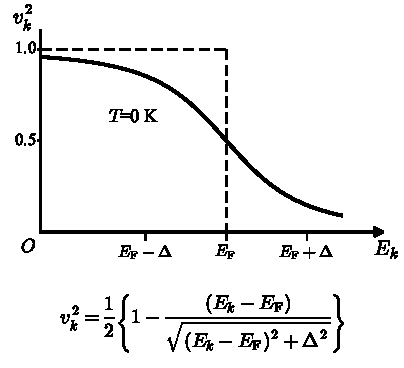
\includegraphics[width=5.5cm]{fig6-6.pdf}\\{\small 图 6.6\quad 超导体中的零温粒子分布}
\end{minipage}
\end{center}

\subsection*{4. 超导体中的元激发}

从BCS超导体的对角化哈密顿量
\begin{equation*}
  \overline{H}=E_{\mathrm{s}}
  +\sum_{k}\xi_{k}\left(\alpha^{+}_{k}\alpha_{k}
  +\alpha^{+}_{-k}\alpha_{-k}\right)
\end{equation*}
可知，对于单准粒子激发态
\begin{equation}
  |1_{k}\rangle=\alpha^{+}_{k}|0\rangle
\end{equation}
其元激发能量为
\begin{equation}
  \langle1_{k}|\overline{H}|1_{k}\rangle
  -\langle0|\overline{H}|0\rangle=\xi_{k}
  =\sqrt{\varepsilon_{k}^{2}+\Delta^{2}}
\end{equation}
在费密面上 $\varepsilon_{k}=\varepsilon_{\mathrm{F}}=0$，这时
\begin{equation}
  \xi_{k}=\xi_{\mathrm{F}}=\Delta
\end{equation}
$\Delta$ 是单个准粒子激发所需的最小能量，而任意k的单准粒子激发能为 $\xi_{k}$.由于准粒子算符 $\alpha^{+}_{k}=u_{k}C^{+}_{k}-v_{k}C_{-k}$ 代表电子与空穴的混合，因此既存在"电子"型也存在"空穴"型的准粒子激发.当元激发使系统总粒子数从 $N\to N+1$ 时，超导体中产生"电子"型元激发，而当 $N\to N-1$ 时，产生"空穴"型激发，它们所需的最小能量都是 $\Delta$.实验上可以通过超导体(S)与正常金属(N)的隧道效应，注入电子或空穴，形成"电子"型或"空穴"型元激发.

现在作图像说明\textsuperscript{[3]}：首先考虑超导态是费密面附近电子形成库柏对，并近似认为这些对大致分布在化学势 $\mu$（或费密能 $E_{\mathrm{F}}$）上，由于超导体中准粒子激发能为 $\xi_{k}$，相对于 $\mu$（或 $E_{\mathrm{F}}$）作 $\xi_{k}$ 曲线，如图6.7所示，它可以作为说明超导元激发的图像.图6.8是正常金属与超导体N-S接触的能谱图像，其中(a)为偏压 $V=0$ 情况，这时N-S结两边化学势相等，而(b)为加正向偏压情况.当 $eV\geqslant\Delta$ 时可从N向S注入电子产生"电子型"元激发，若加反向偏压［如图(c)］，则只有当 $e|V|\geqslant\Delta$ 时，超导体中取出一个电子所得到的能量才足够使剩下的配偶电子激发到 $\xi_{k}$ 曲线上去，这就是注入空穴情况.因此，"电子"型或"空穴"型激发所需最小能量都是 $\Delta$.

\begin{center}
\begin{minipage}{5cm}
\centering
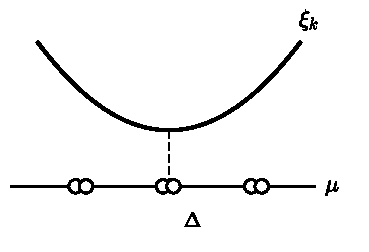
\includegraphics[width=5cm]{fig6-7.pdf}\\{\small 图 6.7\quad 超导体的BCS模型}
\end{minipage}
\end{center}

\begin{center}
\begin{minipage}{8cm}
\centering
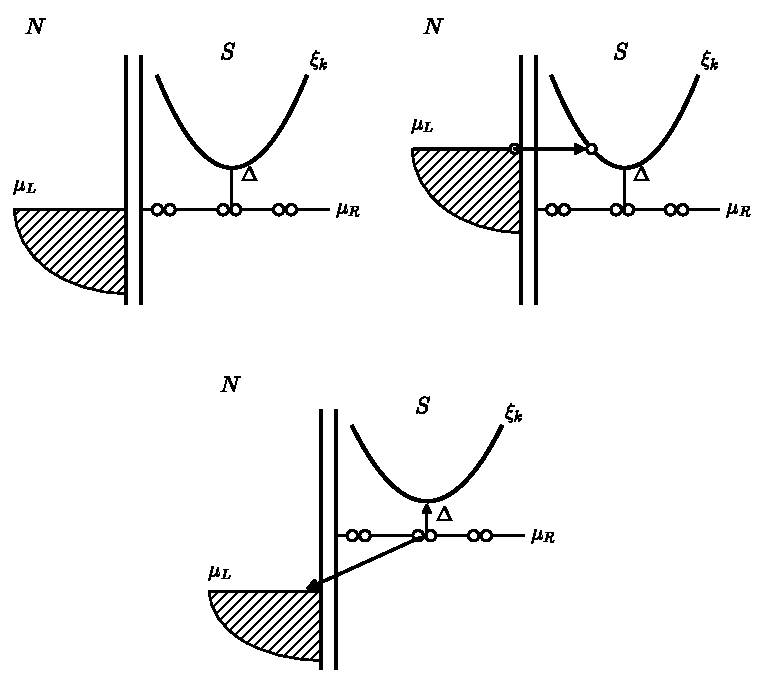
\includegraphics[width=8cm]{fig6-8.pdf}\\[0.3em]
{\small (a) 偏压 $V=0$\qquad\qquad (b) 注入电子 $eV\geqslant\Delta$}\\[0.2em]
{\small (c) 注入空穴 $e|V|\geqslant\Delta$}\\[0.2em]
{\small 图 6.8\quad 超导与正常金属接触}
\end{minipage}
\end{center}

假如在费密面以下激发一个粒子到费密面以上，保持系统总粒子数不变.这时相当于产生了两个准粒子激发，一个是"空穴"型的，一个是"电子"型的.所需最小能量为 $2\Delta$，如图6.9所示，称为电子-空穴对型激发，它相当于拆开一个库柏对.在BCS理论中，电子-空穴对型激发为
\begin{equation}
  \alpha^{+}_{k}\alpha^{+}_{-k}|0\rangle\equiv|\text{对}\rangle
\end{equation}
其元激发能量等于
\begin{equation}
\begin{aligned}
  &\langle\text{对}|\overline{H}|\text{对}\rangle
  -\langle0|\overline{H}|0\rangle\\
  &\quad=\sum_{k'}\xi_{k'}\langle0|\alpha_{-k}\alpha_{k}
  \left(\alpha^{+}_{k'}\alpha_{k'}
  +\alpha^{+}_{-k'}\alpha_{-k'}\right)\alpha^{+}_{k}\alpha^{+}_{-k}|0\rangle
  =2\xi_{k}
\end{aligned}
\end{equation}
同样也说明最小激发能为 $2\Delta$.

\begin{center}
\begin{minipage}{5cm}
\centering
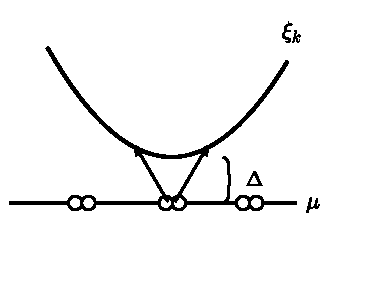
\includegraphics[width=5cm]{fig6-9.pdf}\\{\small 图 6.9\quad 电子-空穴对型激发}
\end{minipage}
\end{center}

\subsection*{5. 超电流}

以上所讨论只是不载流的超导态情况，其中每个库柏对为 $(\boldsymbol{k}\uparrow,-\boldsymbol{k}\downarrow)$，其总动量为 $\hbar\boldsymbol{K}=\hbar\boldsymbol{k}+\hbar(-\boldsymbol{k})=0$，如图6.10(a).由于外场作用将使费密球移动 $\delta\boldsymbol{k}$，相应的库柏对变为 $(\boldsymbol{k}+\delta\boldsymbol{k}\uparrow,-\boldsymbol{k}+\delta\boldsymbol{k}\downarrow)$，其总动量等于 $\hbar(2\delta\boldsymbol{k})$，质心速度为 $\dfrac{\hbar\delta\boldsymbol{k}}{m}$，如图6.10(b)，称为载流超导态.因此库柏对运动的电流密度为
\begin{equation}
  j_{\mathrm{s}}=\frac{n}{2}(-2e)\frac{\hbar\delta k}{m}
  =-\frac{ne\hbar\delta k}{m}
\end{equation}

\begin{center}
\begin{minipage}{9cm}
\centering
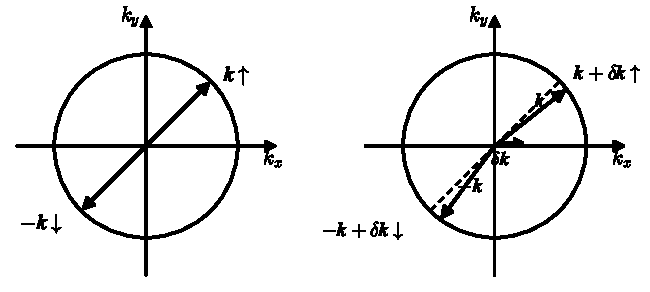
\includegraphics[width=9cm]{fig6-10.pdf}\\[0.3em]
{\small (a) 超导基态\qquad\qquad (b) 载流超导态}\\[0.2em]
{\small 图 6.10\quad 载流超导体中的库柏对}
\end{minipage}
\end{center}

由于互作用只使 $(\boldsymbol{k}+\delta\boldsymbol{k}\uparrow,-\boldsymbol{k}+\delta\boldsymbol{k}\downarrow)$ 库柏对散射为 $(\boldsymbol{k}'+\delta\boldsymbol{k}\uparrow,-\boldsymbol{k}'+\delta\boldsymbol{k}\downarrow)$ 库柏对，总动量不变，即使外场撤去，超导体中仍保持图6.10(b)的组态，因此超导电流 $j_{\mathrm{s}}$ 将不衰减，这说明库柏对所载电流是无阻电流.

$j_{\mathrm{s}}$ 存在一个上限，因为费密球位移 $\delta\boldsymbol{k}$ 将引起动能增加
\begin{equation*}
  \delta\mathcal{E}\approx\left(\frac{n}{2}\right)\frac{1}{2}(2m)
  \left(\frac{\hbar\delta k}{m}\right)^{2}
  =\frac{n\hbar^{2}(\delta k)^{2}}{2m}
\end{equation*}
当 $\delta\mathcal{E}$ 大于凝聚能 $\dfrac{1}{2}g(0)\Delta^{2}$ 时，超导相不再是稳定的，库柏对将被拆散成为正常态，而有电阻，$\delta k$ 的临界值可根据 $\dfrac{n\hbar^{2}(\delta k)_{\mathrm{c}}^{2}}{2m}=\dfrac{1}{2}g(0)\Delta^{2}$ 估计
\begin{equation*}
  |\delta k|_{\mathrm{c}}=\sqrt{\frac{mg(0)}{n}}\left(\frac{\Delta}{\hbar}\right)
  =\sqrt{\frac{3m}{4E_{\mathrm{F}}}}\left(\frac{\Delta}{\hbar}\right)
  \approx\frac{m\Delta}{\hbar^{2}k_{\mathrm{F}}}
\end{equation*}
其中 $g(0)=\dfrac{3n}{4E_{\mathrm{F}}}$.因此，超导电流密度的上限
\begin{equation}
  j_{\mathrm{c}}=\frac{ne\hbar}{m}|\delta k_{\mathrm{c}}|
  \approx\frac{ne\Delta}{\hbar k_{\mathrm{F}}}
\end{equation}
$j_{\mathrm{c}}$ 称为临界电流密度，约为 $10^{7}\,\mathrm{A\,cm^{-2}}$ 量级.这是超导体所能载送的最大电流密度，超导电流满足条件
\begin{equation}
  j_{\mathrm{s}}<\frac{ne}{\hbar k_{\mathrm{F}}}\Delta
\end{equation}
因此，超导体中的无阻电流和能隙的存在直接有关.产生电阻并使 $j_{\mathrm{s}}$ 衰减的弛豫过程，对应于在图6.10(b)中费密球右边留下空穴，而在左边产生电子，相当于从超导态产生两个单粒子型的激发（一个空穴，一个电子），它至少必须有 $2\Delta$ 的能量.当库柏对在外场驱动下的动能 $\dfrac{\hbar k_{\mathrm{F}}}{m}\hbar(2\delta k)<2\Delta$ 时，上述弛豫过程在能量上是不利的，因此不可能发生，这时将得到条件
\begin{equation*}
  \delta k<\frac{m\Delta}{\hbar^{2}k_{\mathrm{F}}}\approx|\delta k_{\mathrm{c}}|
\end{equation*}
它就是
\begin{equation*}
  j_{\mathrm{s}}=\frac{ne\hbar\delta k}{m}
  <\frac{ne\hbar}{m}\frac{m\Delta}{\hbar^{2}k_{\mathrm{F}}}
  =\frac{ne\Delta}{\hbar k_{\mathrm{F}}}
\end{equation*}
以上是BCS理论对超电流的微观解释.这一简单论证不适用于无能隙超导体，其详细讨论见\textsuperscript{[4]}.

\section{有限温度情况}

$T>0$ K时，式(6.4.5)中 $\langle\cdots\rangle$ 代表统计平均 $\langle\cdots\rangle_{T}$，这时存在准粒子的热激发 $\langle\alpha^{+}_{k}\alpha_{k}\rangle_{T}$.因此，有限温度的能隙方程为
\begin{equation}
\begin{aligned}
  \Delta(T)&=V\sum_{k}\langle C_{-k}C_{k}\rangle_{T}\\
  &=V\sum_{k}\langle\left(u_{k}\alpha_{-k}-v_{k}\alpha^{+}_{k}\right)
  \left(u_{k}\alpha_{k}+v_{k}\alpha^{+}_{-k}\right)\rangle_{T}\\
  &=V\sum_{k}u_{k}v_{k}\left(\langle\alpha_{-k}\alpha^{+}_{-k}\rangle_{T}
  -\langle\alpha^{+}_{k}\alpha_{k}\rangle_{T}\right)\\
  &=V\sum_{k}u_{k}v_{k}\left(1-\langle\alpha^{+}_{k}\alpha_{k}\rangle_{T}
  -\langle\alpha^{+}_{-k}\alpha_{-k}\rangle_{T}\right)
\end{aligned}
\end{equation}
由于哈密顿量［式(6.4.23)］已表示为费密算子 $\alpha_{k}$ 的对角形式，$\overline{H}$ 是以 $\xi_{k}$ 为元激发能量的无相互作用准粒子系统.准粒子应当满足费密分布.
\begin{equation}
  \langle\alpha^{+}_{-k}\alpha_{-k}\rangle_{T}
  =\langle\alpha^{+}_{k}\alpha_{k}\rangle_{T}=f(\xi_{k})
  =\left[\exp\left(\frac{\xi_{k}}{k_{\mathrm{B}}T}\right)+1\right]^{-1}
\end{equation}
其中
\begin{equation}
  \xi_{k}=\sqrt{\varepsilon_{k}^{2}+\Delta^{2}(T)}
\end{equation}
$\Delta(T)$ 满足方程
\begin{equation}
  \Delta(T)=V\sum_{k}u_{k}v_{k}\left\{1-2f(\xi_{k})\right\}
\end{equation}
变换系数 $u_{k}$ 与 $v_{k}$ 的形式仍与式(6.4.20)相同，只是其中的 $\Delta=\Delta(0)$ 换成了 $\Delta(T)$
\begin{equation}
  \left.
  \begin{aligned}
    &u_{k}^{2}=\frac{1}{2}\left(1+\frac{\varepsilon_{k}}
    {\sqrt{\varepsilon_{k}^{2}+\Delta^{2}(T)}}\right)\\
    &v_{k}^{2}=\frac{1}{2}\left(1-\frac{\varepsilon_{k}}
    {\sqrt{\varepsilon_{k}^{2}+\Delta^{2}(T)}}\right)
  \end{aligned}\right\}
\end{equation}
将式(6.5.5)代入式(6.5.4)消去 $\Delta(T)$ 因子，求得有限温度的能隙方程为
\begin{equation}
\begin{aligned}
  1&=\frac{1}{2}V\sum_{k}\frac{1-2f(\xi_{k})}{\xi_{k}}\\
  &=\frac{1}{2}V\sum_{k}\frac{\tanh\left(\frac{1}{2}\beta\xi_{k}\right)}{\xi_{k}}
  \qquad\left(\beta=\frac{1}{k_{\mathrm{B}}T}\right)
\end{aligned}
\end{equation}
由式(6.5.6)可以确定能隙与温度关系以及超导转变温度 $T_{\mathrm{c}}$.对于热力学量如熵和比热容等的计算，式(6.5.6)也是必须的自洽条件.

\subsection*{1. 确定$T_{\mathrm{c}}$}

由于 $\Delta(T)\to0$ 时 $\xi_{k}\to|\varepsilon_{k}|$，超导元激发变为正常电子的激发，因此超导正常转变温度 $T_{\mathrm{c}}$ 由条件
\begin{equation}
  \Delta(T_{\mathrm{c}})=0
\end{equation}
决定. $T=T_{\mathrm{c}}$ 时式(6.5.6)可写成
\begin{equation*}
\begin{aligned}
  1&=g(0)V\int_{0}^{\hbar\omega_{\mathrm{D}}}\mathrm{d}\varepsilon\,
  \frac{\tanh\left(\frac{1}{2}\beta_{\mathrm{c}}\varepsilon\right)}{\varepsilon}\\
  &=g(0)V\int_{0}^{\frac{1}{2}\beta_{\mathrm{c}}\hbar\omega_{\mathrm{D}}}
  \mathrm{d}x\,\frac{\tanh x}{x}
\end{aligned}
\end{equation*}
作分部积分
\begin{equation*}
  1=g(0)V\left\{\ln x\tanh x\Bigl|
  _{0}^{\frac{1}{2}\beta_{\mathrm{c}}\hbar\omega_{\mathrm{D}}}
  -\int_{0}^{\frac{1}{2}\beta_{\mathrm{c}}\hbar\omega_{\mathrm{D}}}
  \mathrm{d}x\,\ln x\,\mathrm{sech}^{2}x\right\}
\end{equation*}
其中 $\beta_{\mathrm{c}}=\left(k_{\mathrm{B}}T_{\mathrm{c}}\right)^{-1}$.由于积分是收敛的，并且 $\hbar\omega_{\mathrm{D}}\gg k_{\mathrm{B}}T$，积分的上限可换为 $\infty$，上式可近似为
\begin{equation}
  1=g(0)V\left\{\ln\left(\frac{\hbar\omega_{\mathrm{D}}}{2k_{\mathrm{B}}T_{\mathrm{c}}}\right)
  -\int_{0}^{\infty}\mathrm{d}x\,\ln x\,\mathrm{sech}^{2}x\right\}
\end{equation}
利用欧拉（Euler）积分公式
\begin{equation*}
  \int_{0}^{\infty}\mathrm{d}x\,\ln x\,\mathrm{sech}^{2}x
  =-\ln\frac{4\mathrm{e}^{\gamma}}{\pi}
\end{equation*}
其中 $\gamma\approx0.5772$ 是欧拉常数，$\dfrac{2\mathrm{e}^{\gamma}}{\pi}\approx1.13$，可把式(6.5.8)简化为
\begin{equation}
  1=g(0)V\ln\left[\left(\frac{2\mathrm{e}^{\gamma}}{\pi}\right)
  \left(\frac{\hbar\omega_{\mathrm{D}}}{k_{\mathrm{B}}T_{\mathrm{c}}}\right)\right]
\end{equation}
从而求得
\begin{equation}
\begin{aligned}
  k_{\mathrm{B}}T_{\mathrm{c}}&=\frac{2\mathrm{e}^{\gamma}}{\pi}
  \hbar\omega_{\mathrm{D}}\exp\Bigl[-\frac{1}{g(0)V}\Bigr]\\
  &\approx 1.13\,\hbar\omega_{\mathrm{D}}
  \exp\Bigl[-\frac{1}{g(0)V}\Bigr]
\end{aligned}
\end{equation}
上式与零温能隙公式(6.4.29)相比较，得到BCS超导体的一个普适关系式
\begin{equation}
  \frac{2\Delta(0)}{k_{\mathrm{B}}T_{\mathrm{c}}}=2\pi\mathrm{e}^{-\gamma}
  \approx 3.53
\end{equation}
$2\pi\mathrm{e}^{-\gamma}$ 是与材料特性无关的常数.除Pb以外，这个结果与实验基本符合，如表6.1所示.

由于声子的德拜频率 $\omega_{\mathrm{D}}\sim M^{-1/2}$，M为金属离子质量，则式(6.5.10)给出 $T_{\mathrm{c}}M^{\frac{1}{2}}=$ 常数的同位素效应公式.

\subsection*{2. 能隙与温度关系}

为了求得 $\Delta(T)$，应求下列积分方程的数值解：
\begin{equation}
\begin{aligned}
  1&=\frac{1}{2}V\sum_{k}\frac{1}{\sqrt{\varepsilon_{k}^{2}+\Delta^{2}(T)}}
  -V\sum_{k}\frac{1}{\sqrt{\varepsilon_{k}^{2}+\Delta^{2}(T)}}\times\\
  &\quad\left[\exp\bigl(\beta\sqrt{\varepsilon_{k}^{2}+\Delta^{2}(T)}\bigr)+1\right]^{-1}
\end{aligned}
\end{equation}
当 $T\to0$ 时，$\{\cdots\}^{-1}\to0$，上式变为
\begin{equation}
\begin{aligned}
  1&=\frac{1}{2}V\sum_{k}\frac{1}{\sqrt{\varepsilon_{k}^{2}+\Delta^{2}(T)}}
  =g(0)V\,\mathrm{arsinh}\,\frac{\hbar\omega_{\mathrm{D}}}{\Delta(0)}\\
  &\approx g(0)V\ln\frac{2\hbar\omega_{\mathrm{D}}}{\Delta(0)}
\end{aligned}
\end{equation}
求得的 $\Delta(0)$ 与式(6.4.28)一致.

式(6.5.12)右边第一项可改写成
\begin{equation*}
  g(0)V\ln\frac{2\hbar\omega_{\mathrm{D}}}{\Delta(T)}
\end{equation*}
再利用式(6.5.13)将积分方程(6.5.12)表示为
\begin{equation}
\begin{aligned}
  \ln\left[\frac{\Delta(0)}{\Delta(T)}\right]
  &=2\int_{0}^{\hbar\omega_{\mathrm{D}}}
  \frac{\mathrm{d}\varepsilon}{\sqrt{\varepsilon^{2}+\Delta^{2}(T)}}\times\\
  &\quad\frac{1}{\left[\exp\bigl(\beta\sqrt{\varepsilon^{2}+\Delta^{2}(T)}\bigr)+1\right]}
\end{aligned}
\end{equation}
上式表明随着温度升高 $\Delta(T)$ 单调减小.由于 $\hbar\omega_{\mathrm{D}}\gg k_{\mathrm{B}}T$（$0\leqslant T\leqslant T_{\mathrm{c}}$），存在着近似关系式
\begin{equation}
\begin{aligned}
  \ln\left[\frac{\Delta(T)}{\Delta(0)}\right]
  &=-2\int_{0}^{\infty}\mathrm{d}x\,
  \frac{1}{\sqrt{x^{2}+\left(\dfrac{\Delta(T)}{k_{\mathrm{B}}T}\right)^{2}}}\times\\
  &\quad\frac{1}{\left[\exp\sqrt{x^{2}+\left(\dfrac{\Delta(T)}{k_{\mathrm{B}}T}\right)^{2}}\right]+1}
\end{aligned}
\end{equation}
因此 $\dfrac{\Delta(T)}{\Delta(0)}$ 是 $\dfrac{k_{\mathrm{B}}T}{\Delta(0)}$ 或 $\dfrac{T}{T_{\mathrm{c}}}$ 的普适函数，其数值计算结果如图6.11，与实验测量相符.

\begin{center}
\begin{minipage}{6.5cm}
\centering
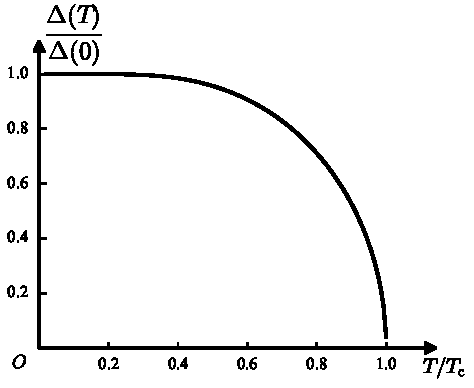
\includegraphics[width=6.5cm]{fig6-11.pdf}\\{\small 图 6.11\quad 能隙与温度关系}
\end{minipage}
\end{center}

当 $T\ll T_{\mathrm{c}}$ 时，由于 $\Delta(T)\approx\Delta(0)$，式(6.5.14)可写成
\begin{equation*}
  \ln\left[\frac{\Delta(T)}{\Delta(0)}\right]
  =-2\int_{0}^{\hbar\omega_{\mathrm{D}}}\mathrm{d}\varepsilon\,
  \frac{\exp\bigl[-\beta\sqrt{\varepsilon^{2}+\Delta^{2}(0)}\bigr]}
  {\sqrt{\varepsilon^{2}+\Delta^{2}(0)}}
\end{equation*}
考虑到 $\beta\Delta(0)\gg1$，积分中指数因子迅速衰减，故 $\varepsilon\approx0$ 对积分贡献最大.这时 $\sqrt{\varepsilon^{2}+\Delta^{2}(0)}$ 可按照 $\dfrac{\varepsilon}{\Delta(0)}$ 展开，其近似结果为
\begin{equation}
\begin{aligned}
  \ln\left[\frac{\Delta(T)}{\Delta(0)}\right]
  &=-\frac{2}{\Delta(0)}\int_{0}^{\hbar\omega_{\mathrm{D}}}\mathrm{d}\varepsilon\,
  \mathrm{e}^{-\frac{\Delta(0)}{k_{\mathrm{B}}T}
  \left(1+\frac{\varepsilon^{2}}{2\Delta^{2}(0)}\right)}\\
  &=-\frac{2}{\Delta(0)}\left[2k_{\mathrm{B}}T\Delta(0)\right]^{1/2}
  \mathrm{e}^{-\frac{\Delta(0)}{k_{\mathrm{B}}T}}
  \int_{0}^{\infty}\mathrm{d}x\,\mathrm{e}^{-x^{2}}\\
  &=-\left(\frac{2\pi k_{\mathrm{B}}T}{\Delta(0)}\right)^{1/2}
  \mathrm{e}^{-\frac{\Delta(0)}{k_{\mathrm{B}}T}}
\end{aligned}
\end{equation}
又因为 $T\ll T_{\mathrm{c}}$ 时，$\Delta(0)-\Delta(T)\ll\Delta(0)$，因此有
\begin{equation*}
  \ln\frac{\Delta(T)}{\Delta(0)}
  =\ln\left(1-\frac{\Delta(0)-\Delta(T)}{\Delta(0)}\right)
  \approx\frac{\Delta(T)-\Delta(0)}{\Delta(0)}
\end{equation*}
可求得 $\Delta(T)$ 的低温近似式
\begin{equation}
  \Delta(T)\approx\Delta(0)-\left[2\pi k_{\mathrm{B}}T\Delta(0)\right]^{1/2}
  \mathrm{e}^{-\frac{\Delta(0)}{k_{\mathrm{B}}T}}
  \qquad(T\ll T_{\mathrm{c}})
\end{equation}
为导出 $T\to T_{\mathrm{c}}$ 时能隙 $\Delta(T)$ 的近似式，最好从自洽方程(6.5.6)出发
\begin{equation}
\begin{aligned}
  1&=g(0)V\int_{0}^{\hbar\omega_{\mathrm{D}}}
  \frac{\tanh\left(\frac{1}{2}\beta\xi\right)}{\xi}\,\mathrm{d}\varepsilon\\
  &=g(0)V\int_{0}^{\hbar\omega_{\mathrm{D}}}
  \frac{f(-\xi)-f(\xi)}{\xi}\,\mathrm{d}\varepsilon
\end{aligned}
\end{equation}
利用泊松求和公式\footnote{详见附录E.}
\begin{equation}
\begin{aligned}
  f(\xi)&=k_{\mathrm{B}}T\sum_{n=-\infty}^{\infty}
  \frac{\mathrm{e}^{\mathrm{i}\omega_{n}\eta}}{\mathrm{i}\omega_{n}-\xi}\\
  \omega_{n}&=(2n+1)\pi k_{\mathrm{B}}T\qquad(n=\text{整数})
\end{aligned}
\end{equation}
并令 $\eta\to+0$，求得
\begin{equation}
  \frac{\tanh\left(\frac{1}{2}\beta\varepsilon\right)}{\varepsilon}
  =\frac{f(-\varepsilon)-f(\varepsilon)}{\varepsilon}
  =4k_{\mathrm{B}}T\sum_{n=0}^{\infty}
  \frac{1}{\omega_{n}^{2}+\varepsilon^{2}+\Delta^{2}(T)}
\end{equation}
代入式(6.5.18)，将自洽方程用下列级数的积分表示：
\begin{equation}
  1=4k_{\mathrm{B}}Tg(0)V\int_{0}^{\hbar\omega_{\mathrm{D}}}\mathrm{d}\varepsilon
  \sum_{n=0}^{\infty}
  \frac{1}{\omega_{n}^{2}+\varepsilon^{2}+\Delta^{2}(T)}
\end{equation}
用上式便于求近似.由于 $T\to T_{\mathrm{c}}$ 时 $\Delta(T)\to0$，可令 $\Delta$ 为小参量，并将上式按 $\Delta(T)$ 展开，得
\begin{equation}
\begin{aligned}
  1&=4k_{\mathrm{B}}Tg(0)V\sum_{n=0}^{\infty}\int_{0}^{\hbar\omega_{\mathrm{D}}}
  \mathrm{d}\varepsilon\left\{\frac{1}{\left(\omega_{n}^{2}+\varepsilon^{2}\right)}
  -\frac{\Delta^{2}(T)}{\left(\omega_{n}^{2}+\varepsilon^{2}\right)^{2}}+\cdots\right\}\\
  &=g(0)V\left\{\int_{0}^{\hbar\omega_{\mathrm{D}}}\mathrm{d}\varepsilon\,
  \frac{\tanh\left(\frac{1}{2}\beta\varepsilon\right)}{\varepsilon}
  -4k_{\mathrm{B}}T\Delta^{2}(T)\sum_{n=0}^{\infty}
  \int_{0}^{\hbar\omega_{\mathrm{D}}}
  \frac{\mathrm{d}\varepsilon}{\left(\omega_{n}^{2}+\varepsilon^{2}\right)^{2}}\right\}
\end{aligned}
\end{equation}
利用欧拉积分，求得式中的
\begin{equation}
  \int_{0}^{\hbar\omega_{\mathrm{D}}}\mathrm{d}\varepsilon\,
  \frac{\tanh\left(\frac{1}{2}\beta\varepsilon\right)}{\varepsilon}
  =\ln\left[\left(\frac{2\mathrm{e}^{\gamma}}{\pi}\right)
  \left(\frac{\hbar\omega_{\mathrm{D}}}{k_{\mathrm{B}}T}\right)\right]
\end{equation}
再根据式(6.5.9)将式(6.5.22)写成
\begin{equation}
\begin{aligned}
  \ln\left(\frac{T}{T_{\mathrm{c}}}\right)
  &=-4k_{\mathrm{B}}T\Delta^{2}(T)\sum_{n=0}^{\infty}
  \int_{0}^{\hbar\omega_{\mathrm{D}}}\mathrm{d}\varepsilon\,
  \frac{1}{\left(\omega_{n}^{2}+\varepsilon^{2}\right)^{2}}\\
  &\approx-\left[\frac{\Delta(T)}{\pi k_{\mathrm{B}}T}\right]^{2}
  \sum_{n=0}^{\infty}\frac{1}{(2n+1)^{3}}
\end{aligned}
\end{equation}
等式右边的级数可用黎曼 $\zeta$ 函数表示，因为
\begin{equation}
  \sum_{n=0}^{\infty}\frac{1}{(2n+1)^{3}}=\frac{7}{8}\zeta(3)
\end{equation}
其中 $\zeta(3)=1.202$ 是黎曼 $\zeta$ 函数.当 $T_{\mathrm{c}}-T\ll T_{\mathrm{c}}$ 时，有下列近似关系：
\begin{equation}
  \ln\left(\frac{T}{T_{\mathrm{c}}}\right)
  =\ln\left(1+\frac{T-T_{\mathrm{c}}}{T_{\mathrm{c}}}\right)
  \approx-\left(1-\frac{T}{T_{\mathrm{c}}}\right)
\end{equation}
代入式(6.5.24)，即可求出 $T\to T_{\mathrm{c}}$ 时能隙的近似式为
\begin{subequations}
\begin{equation}
  \Delta(T)=\pi k_{\mathrm{B}}T_{\mathrm{c}}
  \sqrt{\frac{8}{7\zeta(3)}}\left(1-\frac{T}{T_{\mathrm{c}}}\right)^{1/2}
  \approx 3.06\,k_{\mathrm{B}}T_{\mathrm{c}}
  \left(1-\frac{T}{T_{\mathrm{c}}}\right)^{1/2}
  \qquad(T_{\mathrm{c}}-T\ll T_{\mathrm{c}})
\end{equation}
利用普适关系式(6.5.11)，上式也可写成
\begin{equation}
  \Delta(T)=\Delta(0)\sqrt{\frac{8}{7\zeta(3)}}
  \left(1-\frac{T}{T_{\mathrm{c}}}\right)^{1/2}
  \qquad(T_{\mathrm{c}}-T\ll T_{\mathrm{c}})
\end{equation}
\end{subequations}
以上结果与分子场理论求得的磁化强度公式相似，这是因为 $\left[M(T)/M(0)\right]$ 和 $\left[\Delta(T)/\Delta(0)\right]$ 都是系统的序参量.

\subsection*{3. 热力学量}

表6.1\quad 某些超导金属的热力学量

\begin{center}\small
\begin{tabular}{lcccccc}
\hline
金属 & $T_{\mathrm{c}}$/K &
$\theta_{\mathrm{D}}=\dfrac{\hbar\omega_{\mathrm{D}}}{k_{\mathrm{B}}}$/K &
$g(0)V$ & $\Delta(0)$/eV &
$2\Delta(0)/k_{\mathrm{B}}T_{\mathrm{c}}$ &
$\left(\dfrac{c_{\mathrm{es}}-c_{\mathrm{en}}}{c_{\mathrm{en}}}\right)_{T_{\mathrm{c}}}$\\
\hline
Cd & 0.56 & 164 & 0.18 & $0.75\times10^{-4}$ & 3.2～3.4 & 1.32～1.40\\
Al & 1.2 & 375 & 0.18 & 1.70 & 3.4～3.5 & 1.45\\
Ga & 1.09 & 240 & 0.19 & 1.65 & 3.52 & 1.44\\
Tl & 2.4 & 100 & 0.27 & 3.68 & 3.58 & 1.50\\
In & 3.4 & 109 & 0.29 & 5.25 & 3.61 & 1.73\\
Sn & 3.75 & 195 & 0.25 & 5.75 & 3.51 & 1.60\\
V & 4.9 & 338 & 0.24 & 8.00 & 3.50 & 1.49\\
Pb & 7.22 & 96 & 0.39 & 13.7 & 4.38 & 2.71\\
\hline
\end{tabular}
\end{center}

吉布斯函数
\begin{equation}
  G_{\mathrm{s}}(T)=-k_{\mathrm{B}}T\ln Z
  =-k_{\mathrm{B}}T\ln\mathrm{Tr}\,\mathrm{e}^{-\beta\overline{H}}
\end{equation}
其中 $\overline{H}$ 的c数项在有限温度时可按照(6.4.24)改写为
\begin{equation}
  2\sum_{k}\varepsilon_{k}v_{k}^{2}
  -2\Delta(T)\sum_{k}u_{k}v_{k}
  +\frac{\Delta^{2}(T)}{V}
\end{equation}
代入 $u_{k}$ 和 $v_{k}$ 的表示式(6.5.5)，并利用式(6.5.3)，得
\begin{equation}
  \sum_{k}\left\{\varepsilon_{k}
  -\sqrt{\varepsilon_{k}^{2}+\Delta^{2}(T)}\right\}
  +\frac{\Delta^{2}(T)}{V}
\end{equation}
$\overline{H}$ 中含准粒子算符部分为
\begin{equation}
  -k_{\mathrm{B}}T\ln\mathrm{Tr}\,\exp\left\{-\beta\sum_{k}\xi_{k}
  \left(\alpha^{+}_{k}\alpha_{k}+\alpha^{+}_{-k}\alpha_{-k}\right)\right\}
\end{equation}
由于 $\xi_{-k}=\xi_{k}$，并且求和中各项独立，不难证明它等于
\begin{equation}
  -2k_{\mathrm{B}}T\ln\prod_{k}\mathrm{Tr}\,\exp\left(-\beta\xi_{k}
  \alpha^{+}_{k}\alpha_{k}\right)
\end{equation}
而
\begin{equation}
  \mathrm{Tr}\,\exp\left(-\beta\xi_{k}\alpha^{+}_{k}\alpha_{k}\right)\equiv
  \sum_{n}\langle n|\exp\left(-\beta\xi_{k}\alpha^{+}_{k}\alpha_{k}\right)|n\rangle
\end{equation}
其中 $\alpha^{+}_{k}\alpha_{k}|n\rangle=n|n\rangle$，对于费密子系统 $n=0$，$1$，则从式(6.5.33)可算出
\begin{equation}
\begin{aligned}
  \mathrm{Tr}\,\exp\left(-\beta\xi_{k}\alpha^{+}_{k}\alpha_{k}\right)
  &=\langle0|\exp\left(-\beta\xi_{k}\alpha^{+}_{k}\alpha_{k}\right)|0\rangle
  +\langle1|\exp\left(-\beta\xi_{k}\alpha^{+}_{k}\alpha_{k}\right)|1\rangle\\
  &=1+\mathrm{e}^{-\beta\xi_{k}}=\left(1-f_{k}\right)^{-1}
\end{aligned}
\end{equation}
这里 $f_{k}$ 为准粒子占据数
\begin{equation}
  f_{k}\equiv f(\xi_{k})=\left(\mathrm{e}^{\beta\xi_{k}}+1\right)^{-1}
\end{equation}
因此，式(6.5.32)可写成
\begin{equation}
  2k_{\mathrm{B}}T\sum_{k}\ln\left(1-f_{k}\right)
\end{equation}
它代表独立费密子（准粒子）系的自由能.式(6.5.36)与式(6.5.30)之和即BCS的吉布斯函数
\begin{equation}
  G_{\mathrm{s}}(T)=2k_{\mathrm{B}}T\sum_{k}\ln\left(1-f_{k}\right)
  +\sum_{k}\left\{\varepsilon_{k}
  -\sqrt{\varepsilon_{k}^{2}+\Delta^{2}(T)}\right\}
  +\frac{\Delta^{2}(T)}{V}
\end{equation}
由此可定出超导体中电子的熵
\begin{equation}
\begin{aligned}
  S_{\mathrm{es}}&=-\frac{\partial G_{\mathrm{s}}}{\partial T}\\
  &=-2k_{\mathrm{B}}\sum_{k}\left\{(1-f_{k})\ln(1-f_{k})
  +f_{k}\ln f_{k}\right\}\\
  &\quad+\Delta\frac{\partial\Delta}{\partial T}
  \left\{\sum_{k}\frac{1-2f_{k}}{\xi_{k}}-\frac{2}{V}\right\}\\
  &=-2k_{\mathrm{B}}\sum_{k}\left[(1-f_{k})\ln(1-f_{k})+f_{k}\ln f_{k}\right]
\end{aligned}
\end{equation}
超导体的电子比热容
\begin{equation}
\begin{aligned}
  c_{\mathrm{es}}&=T\frac{\partial S_{\mathrm{es}}}{\partial T}
  =-\beta\frac{\partial S_{\mathrm{es}}}{\partial\beta}\\
  &=2\beta k_{\mathrm{B}}\sum_{k}\frac{\partial f_{k}}{\partial\beta}
  \ln\frac{f_{k}}{1-f_{k}}\\
  &=-2\beta^{2}k_{\mathrm{B}}\sum_{k}\xi_{k}\frac{\partial f_{k}}{\partial\beta}\\
  &=-2\beta^{2}k_{\mathrm{B}}\sum_{k}\xi_{k}
  \frac{\mathrm{d}f_{k}}{\mathrm{d}\left(\beta\xi_{k}\right)}
  \left(\xi_{k}+\beta\frac{\mathrm{d}\xi_{k}}{\mathrm{d}\beta}\right)\\
  &=-2\beta^{2}k_{\mathrm{B}}\sum_{k}\left(-\frac{\partial f_{k}}{\partial\xi_{k}}\right)
  \left(\xi_{k}^{2}+\frac{1}{2}\beta\frac{\mathrm{d}\Delta^{2}(T)}{\mathrm{d}\beta}\right)
\end{aligned}
\end{equation}
其中第二项代表超导能隙引起比热容的变化.不难证明，正是这一项导致 $T=T_{\mathrm{c}}$ 处的电子比热容跃变.因为，在 $T\to T_{\mathrm{c}}$ 时，式(6.5.39)中 $\xi_{k}\to\varepsilon_{k}$，其右边第一项代表正常态电子比热容
\begin{equation}
  2\beta^{2}k_{\mathrm{B}}\sum_{k}\left(-\frac{\partial f}{\partial\xi_{k}}\right)\xi_{k}^{2}
  =2\beta k_{\mathrm{B}}\sum_{k}\left(-\frac{\partial f}{\partial\varepsilon_{k}}\right)
  \varepsilon_{k}^{2}
  =\frac{2\pi^{2}}{3}g(0)k_{\mathrm{B}}^{2}T=c_{\mathrm{en}}
\end{equation}
由此求得 $T=T_{\mathrm{c}}$ 处比热容的跃变为
\begin{equation}
\begin{aligned}
  \Delta c&=\left(c_{\mathrm{es}}-c_{\mathrm{en}}\right)|_{T=T_{\mathrm{c}}}\\
  &=g(0)k_{\mathrm{B}}\beta^{2}\left(\frac{\mathrm{d}\Delta^{2}}{\mathrm{d}\beta}\right)
  \int_{-\infty}^{\infty}\left(-\frac{\partial f}{\partial\varepsilon}\right)
  \mathrm{d}\varepsilon\\
  &=g(0)\left(\frac{-\mathrm{d}\Delta^{2}}{\mathrm{d}T}\right)\Big|_{T=T_{\mathrm{c}}}
\end{aligned}
\end{equation}
利用 $T_{\mathrm{c}}$ 附近 $\Delta(T)$ 的近似式(6.5.27)和 $\Delta(0)$ 公式(6.5.11)，求得 $\Delta c\approx9.4\,g(0)k_{\mathrm{B}}^{2}T_{\mathrm{c}}$，它和式(6.5.40)之比为
\begin{equation}
  \frac{\Delta c}{c_{\mathrm{en}}}=\frac{12}{7\zeta(3)}
  \approx\frac{9.4}{\frac{2}{3}\pi^{2}}=1.43
\end{equation}
对于弱耦合超导体，这也是一个普适关系，并与实验结果一致，具体数据见表6.1.比热容存在跃变说明超导-正常相变是二级相变.

在低温区 $T\ll T_{\mathrm{c}}$ 时，$\Delta(T)\approx\Delta(0)$，这时式(6.5.39)中 $\beta\dfrac{\mathrm{d}\Delta^{2}}{\mathrm{d}\beta}$ 项可略去，而 $\left(-\dfrac{\partial f}{\partial\xi}\right)
=\dfrac{\beta\mathrm{e}^{\beta\xi}}{\left(\mathrm{e}^{\beta\xi}+1\right)^{2}}
\approx\beta\mathrm{e}^{-\beta\xi}$.这时取与式(6.5.16)相似的近似，求得电子比热容的低温近似式
\begin{equation*}
\begin{aligned}
  c_{\mathrm{es}}&\approx 2\beta^{2}k_{\mathrm{B}}\,g(0)
  \int_{-\infty}^{\infty}\mathrm{d}\varepsilon\,\mathrm{e}^{-\beta\xi}\xi^{2}\\
  &\approx 2\beta^{2}k_{\mathrm{B}}\,g(0)\,
  \mathrm{e}^{-\frac{\Delta(0)}{k_{\mathrm{B}}T}}\Delta^{2}(0)
  \int_{-\infty}^{\infty}\mathrm{d}\varepsilon\,
  \mathrm{e}^{-\frac{1}{2}\beta\frac{\varepsilon^{2}}{\Delta(0)}}
\end{aligned}
\end{equation*}
\begin{equation}
  =2g(0)\frac{\Delta^{2}(0)}{T}
  \left[\frac{2\pi\Delta(0)}{k_{\mathrm{B}}T}\right]^{1/2}
  \mathrm{e}^{-\frac{\Delta(0)}{k_{\mathrm{B}}T}}
\end{equation}
上式说明超导态电子的低温比热容是温度的指数函数，与§1中实验结果一致.

\subsection*{4. 超导相变}

在 $\lambda$ 互作用系统 $\overline{H}(\lambda)=\overline{H}_{0}
+\overline{H}_{\mathrm{int}}(\lambda)$ 和 $\overline{H}_{\mathrm{int}}(\lambda)=\lambda\overline{H}_{\mathrm{int}}$ 中，利用吉布斯自由能公式 $G(\lambda)=-k_{\mathrm{B}}T\ln\mathrm{Tr}\,\exp\left[-\beta\overline{H}(\lambda)\right]$ 不难证明 $T>0$ K时的费因曼定理［习题(33)］为
\begin{equation}
  \frac{\partial G(\lambda)}{\partial\lambda}
  =\frac{\langle\overline{H}_{\mathrm{int}}(\lambda)\rangle_{T}}{\lambda}
\end{equation}
在超导问题中，由于 $\overline{H}_{\mathrm{int}}
=-\Delta\sum_{k}\left(C^{+}_{k}C^{+}_{-k}+C_{-k}C_{k}\right)
+\left(\Delta^{2}/V\right)$ 和 $\Delta=V\sum_{k}\langle C_{-k}C_{k}\rangle_{T}$，其中V为互作用常数，则 $\lambda$ 系统的超导能隙方程为
\begin{equation}
  \Delta(\lambda)=\lambda\sum_{k}\langle C_{-k}C_{k}\rangle_{T}
\end{equation}
相应的
\begin{equation}
  \overline{H}_{\mathrm{int}}(\lambda)=-\Delta(\lambda)\sum_{k}
  \left(C^{+}_{k}C^{+}_{-k}+C_{-k}C_{k}\right)
  +\frac{\Delta^{2}(\lambda)}{\lambda}
\end{equation}
因此，$\langle\overline{H}_{\mathrm{int}}(\lambda)\rangle
=-\left[\Delta^{2}(\lambda)/\lambda\right]$，代入式(6.5.44)求得
\begin{equation}
  \frac{\partial G(\lambda)}{\partial\lambda}
  =-\frac{\Delta^{2}(\lambda)}{\lambda^{2}}
\end{equation}
在这里可设
\begin{equation}
  \lambda=\begin{cases}
    0 & \cdots\text{N相}\ \left[\text{因为 }\Delta(\lambda=0)=0\right]\\
    V & \cdots\text{S相}\ \left[\text{因为 }\Delta(\lambda=V)=\Delta(T)\right]
  \end{cases}
\end{equation}
再对 $\lambda$ 从0到V作积分，即可以将超导相与正常相之间的吉布斯自由能之差写成
\begin{equation}
\begin{aligned}
  \Delta G&=G_{\mathrm{S}}-G_{\mathrm{N}}
  =\int_{0}^{V}\mathrm{d}\lambda\left[-\Delta^{2}(\lambda)/\lambda^{2}\right]\\
  &=\int_{0}^{\Delta(T)}\Delta^{2}(\lambda)
  \left[\mathrm{d}(1/\lambda)/\mathrm{d}\Delta(\lambda)\right]
  \mathrm{d}\Delta(\lambda)
\end{aligned}
\end{equation}
其中的 $\left[\mathrm{d}(1/\lambda)/\mathrm{d}\Delta(\lambda)\right]$ 由 $\lambda$ 系统的能隙方程决定
\begin{equation}
  \frac{1}{\lambda}=g(0)\int_{0}^{\Delta(T)}\mathrm{d}\varepsilon
  \left[\frac{\tanh\left(\dfrac{\xi(\lambda)}{2k_{\mathrm{B}}T}\right)}{\xi(\lambda)}\right]
\end{equation}
而
\begin{equation}
  \xi(\lambda)=\sqrt{\varepsilon^{2}+\Delta^{2}(\lambda)}
\end{equation}
这是计算 $\Delta G$ 的一种有效方法，特别是当T趋近于 $T_{\mathrm{c}}$ 时，利用泊松频率求和公式(6.5.19)和(6.5.20)作展开
\begin{equation}
\begin{aligned}
  \frac{1}{\lambda}&=g(0)\int_{0}^{\hbar\omega_{\mathrm{D}}}\mathrm{d}\varepsilon\,
  \left(4k_{\mathrm{B}}T\right)\sum_{n=0}^{\infty}
  \frac{1}{\omega_{n}^{2}+\varepsilon^{2}+\Delta^{2}(\lambda)}\\
  &\approx g(0)\int_{0}^{\hbar\omega_{\mathrm{D}}}\mathrm{d}\varepsilon\,
  \left(4k_{\mathrm{B}}T_{\mathrm{c}}\right)\sum_{n=0}^{\infty}
  \left\{\frac{1}{\left(\omega_{n}^{2}+\varepsilon^{2}\right)}
  -\frac{\Delta^{2}(\lambda)}{\left(\omega_{n}^{2}+\varepsilon^{2}\right)^{2}}\right\}
\end{aligned}
\end{equation}
求得
\begin{equation}
\begin{aligned}
  \frac{\mathrm{d}\left(\dfrac{1}{\lambda}\right)}{\mathrm{d}\Delta(\lambda)}
  &=-g(0)\left(8k_{\mathrm{B}}T_{\mathrm{c}}\right)\Delta(\lambda)
  \sum_{n=0}^{\infty}\int_{0}^{\hbar\omega_{\mathrm{D}}}
  \frac{\mathrm{d}\varepsilon}{\left(\omega_{n}^{2}+\varepsilon^{2}\right)^{2}}\\
  &=-\frac{1}{4}g(0)\Delta(\lambda)\,7\zeta(3)
  \left(\pi k_{\mathrm{B}}T_{\mathrm{c}}\right)^{-2}
\end{aligned}
\end{equation}
再代入式(6.5.49)，并利用能隙公式(6.5.27)，可将 $T_{\mathrm{c}}$ 附近吉布斯自由能的变化表示为
\begin{equation}
  \Delta G=G_{\mathrm{S}}-G_{\mathrm{N}}
  =-\frac{1}{2}g(0)\left[\frac{8\pi^{2}k_{\mathrm{B}}^{2}}{7\zeta(3)}\right]
  \left(T_{\mathrm{c}}-T\right)^{2}
\end{equation}
利用上式可讨论 $T_{\mathrm{c}}$ 附近诸热力学量的变化特征，例如

（i）熵变化 $\Delta S=S_{\mathrm{S}}-S_{\mathrm{N}}$

利用热力学关系 $\Delta S=-\partial(\Delta G)/\partial T$，立刻求得
\begin{equation}
  \Delta S=-g(0)\left[\frac{8\pi^{2}k_{\mathrm{B}}^{2}}{7\zeta(3)}\right]
  \left(T_{\mathrm{c}}-T\right)
\end{equation}
此结果表明：当 $T=T_{\mathrm{c}}$ 时 $\Delta S=0$，无潜热，超导(S)-正常(N)转变为二级相变；当 $T<T_{\mathrm{c}}$ 时 $\Delta S\neq0$，有潜热，这时加外磁场可使S相转变为N相，并观测到潜热，属于一级相变.

（ii）电子的比热容跃变
\begin{equation}
  \Delta c=\left[T\left(\frac{\partial\Delta S}{\partial T}\right)\right]_{T=T_{\mathrm{c}}}
  =g(0)\left[\frac{8\pi^{2}k_{\mathrm{B}}^{2}}{7\zeta(3)}\right]T_{\mathrm{c}}
\end{equation}
与用式(6.5.41)计算的结果一致，再利用式(6.5.40)，可导出BCS理论的另一个普适关系式(6.5.42)
\begin{equation*}
  \frac{\Delta c}{c_{\mathrm{en}}}
  =\left[\frac{12}{7\zeta(3)}\right]\approx1.43
\end{equation*}
在 $T_{\mathrm{c}}$ 处存在比热容跃变，进一步证实了 $T=T_{\mathrm{c}}$ 时的S-N转变是二级相变.

（iii）临界磁场 $H_{\mathrm{c}}(T)$

由于在 $T_{\mathrm{c}}$ 附近
\begin{equation*}
  G_{\mathrm{s}}-G_{\mathrm{N}}=-\frac{H_{\mathrm{c}}^{2}(T)}{8\pi}
  =-\frac{1}{2}g(0)\left[\frac{8\pi^{2}k_{\mathrm{B}}^{2}}{7\zeta(3)}\right]
  \left(T_{\mathrm{c}}-T\right)^{2}
\end{equation*}
利用 $H_{\mathrm{c}}(0)=\Delta(0)\sqrt{4\pi g(0)}$ 及普适关系 $\pi k_{\mathrm{B}}T_{\mathrm{c}}=\mathrm{e}^{\gamma}\Delta(0)$，立刻求得BCS理论的超导临界磁场为
\begin{subequations}
\begin{equation}
\begin{aligned}
  H_{\mathrm{c}}(T)&=H_{\mathrm{c}}(0)\mathrm{e}^{\gamma}
  \sqrt{\frac{8}{7\zeta(3)}}\left(1-\frac{T}{T_{\mathrm{c}}}\right)\\
  &\approx1.74\,H_{\mathrm{c}}(0)\left(1-\frac{T}{T_{\mathrm{c}}}\right)
  \qquad(T_{\mathrm{c}}-T\ll T_{\mathrm{c}})
\end{aligned}
\end{equation}
在低温区，当 $T\ll T_{\mathrm{c}}$ 时，从吉布斯自由能公式(6.5.28)出发，利用低温时的常规展开方法［习题32］易求出BCS理论的低温临界磁场公式
\begin{equation}
\begin{aligned}
  H_{\mathrm{c}}(T)&=H_{\mathrm{c}}(0)\left[1-\frac{\mathrm{e}^{2\gamma}}{3}
  \left(\frac{T}{T_{\mathrm{c}}}\right)^{2}\right]\\
  &\approx H_{\mathrm{c}}(0)\left[1-1.06\left(\frac{T}{T_{\mathrm{c}}}\right)^{2}\right]
\end{aligned}
\end{equation}
\end{subequations}
以上结果与临界磁场的经验公式
\begin{equation}
  H_{\mathrm{c}}(T)=H_{\mathrm{c}}(0)
  \left[1-\left(\frac{T}{T_{\mathrm{c}}}\right)^{2}\right]
\end{equation}
相近.但仔细比较BCS公式(6.5.57)与经验公式(6.5.58)，不难看出在低温区 $\left(T\ll T_{\mathrm{c}}\right)$ 与高温区 $\left(T_{\mathrm{c}}-T\ll T_{\mathrm{c}}\right)$ 经验公式均偏大.为了证实哪一个公式更接近实验，在BCS理论问世以后，人们对两者的差异作了实验性的判断，即定义
\begin{equation}
  D(T)\equiv\left\{\frac{H_{\mathrm{c}}(T)}{H_{\mathrm{c}}(0)}
  -\left[1-\left(\frac{T}{T_{\mathrm{c}}}\right)^{2}\right]\right\}
\end{equation}
并作出D(T)与 $\left(T/T_{\mathrm{c}}\right)^{2}$ 曲线，如图6.12所示.若经验公式正确，则应有 $D(T)=0$，而BCS理论曲线则用虚线表示.实验的结果（实线）表明多数的超导元素 $D(T)<0$ 与BCS理论结果式(6.5.57)更为接近，这是理论的成功之处.但是也有例外，对于Pb等少数超导金属，实验曲线为 $D(T)>0$，与BCS理论差别较大，相应地在Pb中 $2\Delta(0)$ 与 $k_{\mathrm{B}}T_{\mathrm{c}}$ 的比值为4.38、量纲为1的比热容跃变 $\left(\Delta c/c_{\mathrm{en}}\right)$ 为2.71，也都分别地相对于BCS的普适关系值3.53与1.43有较大的偏离.

\begin{center}
\begin{minipage}{6cm}
\centering
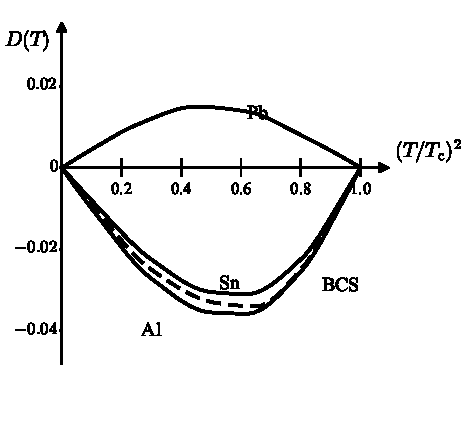
\includegraphics[width=6cm]{fig6-12.pdf}\\{\small 图 6.12\quad 实际临界磁场 $H_{\mathrm{c}}(T)/H_{\mathrm{c}}(0)$ 与经验曲线
$\left[1-(T/T_{\mathrm{c}})^{2}\right]$ 的差别}
\end{minipage}
\end{center}

这是由于Pb中的电子与声子耦合较强，基于二级微扰的BCS约化哈密顿量不再是良好的出发模型，而必须考虑耦合的高阶效应.对于强电声子耦合情形，必须从更为基本的电子与声子相互作用模型出发，运用格林函数技巧，考虑电子-声子-电子间互作用的推迟效应，屏蔽库仑作用以及热声子的激发等效应，才能给出与实验一致的结果，称为强耦合超导理论\textsuperscript{[5]}，而本章中所介绍的BCS理论则称为弱耦合的超导理论，它只适用于 $g(0)V\ll1$ 的情形.

\section{单粒子隧道效应}

利用超导与正常金属间的隧道效应，可直接测定能隙 $\Delta$，并验证BCS的态密度公式.本节着重讨论S-N系统的单粒子隧道效应\textsuperscript{[5]}.

设 $H_{1}$，$H_{2}$ 分别代表两块金属（1、2）的哈密顿量，它们的本征态为 $|\lambda_{1}\rangle$、$|\mu_{2}\rangle$，相应的能量本征值为 $\varepsilon_{\lambda}$ 和 $\varepsilon_{\mu}$
\begin{equation}
  H_{1}|\lambda_{1}\rangle=\varepsilon_{\lambda}|\lambda_{1}\rangle\text{，}
  \qquad H_{2}|\mu_{2}\rangle=\varepsilon_{\mu}|\mu_{2}\rangle
\end{equation}
电子在1、2两种金属间转移的隧道哈密顿量
\begin{equation}
  H_{\mathrm{T}}=\sum_{k,\,k'}\left(\mathscr{M}_{kk'}C^{(2)+}_{k'}C^{(1)}_{k}
  +\mathrm{h.c.}\right)
\end{equation}
系统的总哈密顿量为
\begin{equation}
  H=H_{1}+H_{2}+H_{\mathrm{T}}
\end{equation}
为简单起见，我们先讨论零温情况.根据含时微扰理论，当两块金属之间外加电压V时，它们的费密能相差为 $eV$，此时跃迁概率为
\begin{equation}
\begin{aligned}
  w_{12}=\frac{2\pi}{\hbar}\sum_{\lambda,\,\mu}
  \bigl|\langle\lambda_{1}|\langle\mu_{2}|
  \sum_{k,\,k'}\mathscr{M}_{kk'}C^{(2)+}_{k'}C^{(1)}_{k}
  |0_{2}\rangle|0_{1}\rangle\bigr|^{2}
  \times\delta\left(\varepsilon_{\lambda}+eV-\varepsilon_{\mu}\right)
\end{aligned}
\end{equation}
其中 $|0_{i}\rangle\ (i=1,2)$ 代表金属(1,2)的基态.这时单粒子隧穿电流
\begin{equation}
  I_{12}=ew_{12}
\end{equation}
由于 $V\ll E_{\mathrm{F}}$，参加跃迁的主要是费密面附近的电子，我们可以假定 $\mathscr{M}_{kk'}$ 近似为与k、$k'$ 无关的常数 $\mathscr{M}$，则式(6.6.4)可进一步简化
\begin{equation}
\begin{aligned}
  w_{12}&=\frac{2\pi}{\hbar}|\mathscr{M}|^{2}
  \int_{-\infty}^{\infty}\mathrm{d}\varepsilon
  \sum_{k,\,\lambda}|\langle\lambda_{1}|C^{(1)}_{k}|0_{1}\rangle|^{2}
  \delta(\varepsilon-\varepsilon_{\lambda})\times\\
  &\quad\sum_{k',\,\mu}|\langle\mu_{2}|C^{(2)+}_{k'}|0_{2}\rangle|^{2}
  \delta(\varepsilon+eV-\varepsilon_{\mu})\\
  &=\frac{2\pi}{\hbar}|\mathscr{M}|^{2}
  \int_{-\infty}^{\infty}\mathrm{d}\varepsilon\,
  N_{1}(\varepsilon)N_{2}(\varepsilon+eV)
\end{aligned}
\end{equation}
这里
\begin{equation}
  N_{1}(\varepsilon)\equiv\sum_{k,\,\lambda}
  |\langle\lambda_{1}|C^{(1)}_{k}|0_{1}\rangle|^{2}
  \delta\left(\varepsilon-\varepsilon_{\lambda}\right)
\end{equation}
\begin{equation}
  N_{2}(\varepsilon+eV)\equiv\sum_{k',\,\mu}
  |\langle\mu_{2}|C^{(2)+}_{k'}|0_{2}\rangle|^{2}
  \delta\left(\varepsilon+eV-\varepsilon_{\mu}\right)
\end{equation}
当1、2均为正常金属时
\begin{equation}
  \sum_{\lambda}|\langle\lambda_{1}|C^{(1)}_{k}|0_{1}\rangle|^{2}
  =\langle F|C^{(1)+}_{k}C^{(1)}_{k}|F\rangle
  =\left[1-\theta(\varepsilon_{k})\right]
\end{equation}
\begin{equation}
  \sum_{\mu}|\langle\mu_{2}|C^{(2)+}_{k'}|0_{2}\rangle|^{2}
  =\langle F|C^{(2)}_{k'}C^{(2)+}_{k'}|F\rangle
  =\theta(\varepsilon_{k'})
\end{equation}
其中 $\theta(\varepsilon)$ 为阶跃函数，即
\begin{equation}
  \theta(\varepsilon)=
  \begin{cases}1&(\varepsilon\geqslant0)\\0&(\varepsilon<0)\end{cases}
\end{equation}
由此求得 $T=0$ K时正常金属的
\begin{equation}
\begin{aligned}
  N_{1}(\varepsilon)&=\sum_{k}\left\{1-\theta(\varepsilon_{k})\right\}
  \delta\left(\varepsilon-\varepsilon_{k}\right)\\
  &=\int\mathrm{d}\varepsilon_{k}\,g_{1}(\varepsilon_{k})
  \left\{1-\theta(\varepsilon_{k})\right\}
  \delta\left(\varepsilon-\varepsilon_{k}\right)\\
  &=g_{1}(\varepsilon)\left\{1-\theta(\varepsilon)\right\}
\end{aligned}
\end{equation}
\begin{equation}
\begin{aligned}
  N_{2}(\varepsilon+eV)
  &=\sum_{k'}\theta\left(\varepsilon_{k'}\right)
  \delta\left(\varepsilon+eV-\varepsilon_{k'}\right)\\
  &=g_{2}(\varepsilon+eV)\,\theta(\varepsilon+eV)
\end{aligned}
\end{equation}
两块正常金属之间的隧穿电流
\begin{equation}
\begin{aligned}
  I_{\mathrm{NN}}&=\frac{2\pi e}{\hbar}|\mathscr{M}|^{2}
  \int_{-\infty}^{\infty}\mathrm{d}\varepsilon\,g_{1}(\varepsilon)\,
  g_{2}(\varepsilon+eV)\left\{1-\theta(\varepsilon)\right\}
  \theta\left(\varepsilon+eV\right)\\
  &=\frac{2\pi e}{\hbar}|\mathscr{M}|^{2}
  \int_{-\infty}^{\infty}\mathrm{d}\varepsilon\,g_{1}(\varepsilon)\,
  g_{2}(\varepsilon+eV)
  \left\{f(\varepsilon)\left[1-f(\varepsilon+eV)\right]\right\}_{T=0}
\end{aligned}
\end{equation}
用费密面上态密度 $g(0)$ 代替 $g(\varepsilon)$，可求得正常态的微分电导与V无关
\begin{equation}
\begin{aligned}
  G_{\mathrm{NN}}&=\left(\frac{\mathrm{d}I_{\mathrm{NN}}}{\mathrm{d}V}\right)_{T=0}
  \approx\frac{2\pi e^{2}}{\hbar}|\mathscr{M}|^{2}
  g_{1}(0)g_{2}(0)\int\mathrm{d}\varepsilon\,\delta\left(\varepsilon+eV\right)\\
  &=\frac{2\pi e^{2}}{\hbar}|\mathscr{M}|^{2}g_{1}(0)g_{2}(0)\equiv A
\end{aligned}
\end{equation}
\begin{equation}
  I_{\mathrm{NN}}(V)=AV
\end{equation}
$I-V$ 为直线关系，满足欧姆定律.

当金属1换为超导体时，应取
\begin{equation*}
  C^{(1)}_{k}=u_{k}\alpha_{k}+v_{k}\alpha^{+}_{-k}
\end{equation*}
此时
\begin{equation}
\begin{aligned}
  \sum_{\lambda}|\langle\lambda_{1}|C^{(1)}_{k}|0_{1}\rangle|^{2}
  &=\langle0_{1}|C^{(1)+}_{k}C^{(1)}_{k}|0_{1}\rangle\\
  &=v_{k}^{2}\ \langle0_{1}|\alpha_{-k}\alpha^{+}_{-k}|0_{1}\rangle=v_{k}^{2}
\end{aligned}
\end{equation}
准粒子能量为 $\xi_{k}=\sqrt{\varepsilon_{k}^{2}+\Delta^{2}}$，则式(6.6.7)写为
\begin{equation*}
\begin{aligned}
  N_{1\mathrm{S}}(\varepsilon)
  &=\sum_{k}v_{k}^{2}\delta\left(\varepsilon-\xi_{k}\right)
  =g_{1}(0)\int_{-\infty}^{\infty}\mathrm{d}\varepsilon_{k}\,
  v_{k}^{2}(\varepsilon_{k})\,\delta\left(\varepsilon-\xi_{k}\right)\\
  &=g_{1}(0)\int_{\Delta}^{\infty}\mathrm{d}\xi_{k}\,
  \left|\frac{\mathrm{d}\varepsilon_{k}}{\mathrm{d}\xi_{k}}\right|
  \left\{v_{k}^{2}(\varepsilon_{k})+v_{k}^{2}(-\varepsilon_{k})\right\}
  \delta\left(\varepsilon-\xi_{k}\right)
\end{aligned}
\end{equation*}
根据 $v_{k}^{2}=\frac{1}{2}\left(1-\frac{\varepsilon_{k}}{\xi_{k}}\right)$，可知 $v_{k}^{2}(-\varepsilon_{k})=u_{k}^{2}(\varepsilon_{k})$.因此，$u_{k}^{2}$ 与 $v_{k}^{2}$ 总是同时出现，上式中 $\{\cdots\}$ 因子简单地等于1.
\begin{equation}
  v_{k}^{2}(\varepsilon_{k})+v_{k}^{2}(-\varepsilon_{k})
  =v_{k}^{2}(\varepsilon_{k})+u_{k}^{2}(\varepsilon_{k})=1
\end{equation}
这时 $N_{1\mathrm{S}}(\varepsilon)$ 就是BCS的超导态密度，即
\begin{equation}
\begin{aligned}
  N_{1\mathrm{S}}(\varepsilon)
  &=g_{1}(0)\left|\frac{\mathrm{d}\varepsilon_{k}}{\mathrm{d}\xi_{k}}\right|_{\xi_{k}=\varepsilon}\\
  &=g_{1}(0)\,\mathrm{Re}\,\frac{|\varepsilon|}{\sqrt{\varepsilon^{2}-\Delta^{2}}}
  =g_{1\mathrm{S}}(\varepsilon)
\end{aligned}
\end{equation}
对于正常金属2，$N_{2}$ 仍由式(6.6.13)决定.这样S-N系统在 $T=0$ K时的单粒子隧穿电流为
\begin{equation}
\begin{aligned}
  I_{\mathrm{SN}}&=\frac{2\pi e}{\hbar}|\mathscr{M}|^{2}
  \int_{-\infty}^{\infty}\mathrm{d}\varepsilon\,
  N_{1\mathrm{S}}(\varepsilon)N_{2\mathrm{N}}(\varepsilon+eV)\\
  &=\frac{2\pi e}{\hbar}|\mathscr{M}|^{2}g_{2}(0)
  \int_{-\infty}^{\infty}\mathrm{d}\varepsilon\,
  g_{1\mathrm{S}}(\varepsilon)\,\theta(\varepsilon+eV)
\end{aligned}
\end{equation}
其微分电导为
\begin{equation}
\begin{aligned}
  G_{\mathrm{SN}}&=\left(\frac{\mathrm{d}I_{\mathrm{SN}}}{\mathrm{d}V}\right)_{T=0}
  =\frac{2\pi e^{2}}{\hbar}|\mathscr{M}|^{2}g_{2}(0)
  \int_{-\infty}^{\infty}\mathrm{d}\varepsilon\,
  g_{1\mathrm{S}}(\varepsilon)\,\delta\left(\varepsilon+eV\right)\\
  &=\frac{2\pi e^{2}}{\hbar}|\mathscr{M}|^{2}g_{1}(0)g_{2}(0)
  \int\mathrm{d}\varepsilon\,\frac{g_{1\mathrm{S}}(\varepsilon)}{g_{1}(0)}
  \,\delta(\varepsilon+eV)\\
  &=A\,\mathrm{Re}\,\frac{|eV|}{\sqrt{(eV)^{2}-\Delta^{2}}}
\end{aligned}
\end{equation}
其中A代表 $G_{\mathrm{NN}}$，由式(6.6.15)决定，注意超导态微分电导与正常态微分电导之比是
\begin{equation}
  \frac{G_{\mathrm{SN}}}{G_{\mathrm{NN}}}
  =\mathrm{Re}\,\frac{|eV|}{\sqrt{(eV)^{2}-\Delta^{2}}}
  =g_{1\mathrm{S}}(\varepsilon)\qquad(\varepsilon=eV)
\end{equation}
测定这个比值将给出超导体中的准粒子态密度.根据式(6.6.21)，还可以导出零温隧穿电流为
\begin{equation}
  I_{\mathrm{SN}}(V)=A\,\mathrm{Re}\sqrt{(eV)^{2}-\Delta^{2}}
\end{equation}
现在讨论有限温度情况.对于 $I_{\mathrm{NN}}$，可根据式(6.6.14)再计入反向电子跃迁项
\begin{equation*}
  \frac{2\pi e}{\hbar}|\mathscr{M}|^{2}\int_{-\infty}^{\infty}
  \mathrm{d}\varepsilon\,g_{1}(\varepsilon)g_{2}(\varepsilon+eV)
  \left[1-f(\varepsilon)\right]f(\varepsilon+eV)
\end{equation*}
求得 $T\neq0$ K时的
\begin{equation}
  I_{\mathrm{NN}}=\frac{2\pi e}{\hbar}|\mathscr{M}|^{2}
  \int_{-\infty}^{\infty}\mathrm{d}\varepsilon\,g_{1}(\varepsilon)\,
  g_{2}(\varepsilon+eV)
  \left[f(\varepsilon)-f(\varepsilon+eV)\right]
\end{equation}
在低温和小电压情况下 $\left(1\ll\beta E_{\mathrm{F}},\,eV\ll E_{\mathrm{F}}\right)$ 这个积分容易算出，其结果近似为式(6.6.16)，与零温情况没有太大差别.

对于S-N系统，式(6.6.17)应换为热平均 $\langle C^{(1)+}_{k}C^{(1)}_{k}\rangle_{T}$，其中 $\langle\alpha_{-k}\alpha^{+}_{-k}\rangle_{T}=1-f(\xi_{k})$.详细讨论的结果与 $I_{\mathrm{NN}}$ 相仿，只需将式(6.6.24)中 $g_{1}(\varepsilon)$ 换成 $g_{1\mathrm{S}}(\varepsilon)$，即是
\begin{equation}
  I_{\mathrm{SN}}=\frac{2\pi e}{\hbar}|\mathscr{M}|^{2}
  \int_{-\infty}^{\infty}\mathrm{d}\varepsilon\,
  g_{1\mathrm{S}}(\varepsilon)\,g_{2\mathrm{N}}(\varepsilon+eV)
  \left[f(\varepsilon)-f(\varepsilon+eV)\right]
\end{equation}
利用式(6.6.19)求得 $T\neq0$ K时的微分电导为
\begin{equation}
\begin{aligned}
  G_{\mathrm{SN}}=\frac{\mathrm{d}I_{\mathrm{SN}}}{\mathrm{d}V}
  =\frac{2\pi e^{2}}{\hbar}|\mathscr{M}|^{2}g_{1}(0)g_{2}(0)
  &\left(\int_{\Delta}^{\infty}\frac{|\varepsilon|}{\sqrt{\varepsilon^{2}-\Delta^{2}}}\,
  \frac{\beta\exp\left[\beta(\varepsilon+eV)\right]}
  {\left\{1+\exp\left[\beta(\varepsilon+eV)\right]\right\}^{2}}\mathrm{d}\varepsilon\right.\\
  \left.+\int_{-\infty}^{-\Delta}\frac{|\varepsilon|}{\sqrt{\varepsilon^{2}-\Delta^{2}}}\,
  \frac{\beta\exp\left[\beta(\varepsilon+eV)\right]}
  {\left\{1+\exp\left[\beta(\varepsilon+eV)\right]\right\}^{2}}\mathrm{d}\varepsilon\right)
\end{aligned}
\end{equation}
式(6.6.26)可按贝塞尔函数展开计算.图6.13中实线为 $T=0$ K的情况，它表明在超导体的准粒子态密度中存在能隙 $\Delta$，虚线为 $T>0$ K时的 $G_{\mathrm{SN}}/G_{\mathrm{NN}}$ 曲线，它与 $T=0$ K情况的主要差别是在 $eV<\Delta$ 区域内仍存在隧穿电流.当 $k_{\mathrm{B}}T\ll\Delta$ 和 $V\to0$ 时，式(6.6.26)容易计算，其近似结果为
\begin{equation*}
\begin{aligned}
  \lim_{\substack{T\to0\\ V\to0}}
  \left[\frac{\mathrm{d}I_{\mathrm{SN}}}{\mathrm{d}V}\right]
  &\approx 2A\int_{-\infty}^{-\Delta}\mathrm{d}\varepsilon\,
  \frac{|\varepsilon|}{\sqrt{\varepsilon^{2}-\Delta^{2}}}\,
  \beta\exp\left(\beta\varepsilon\right)\\
  &\approx 2A\int_{\Delta}^{\infty}\mathrm{d}\varepsilon\,
  \frac{|\varepsilon|}{\sqrt{\varepsilon^{2}-\Delta^{2}}}\,
  \beta\exp\left(-\beta\varepsilon\right)\\
  &=2A\beta\int_{0}^{\infty}\mathrm{d}x\,
  \mathrm{e}^{-\beta\sqrt{x^{2}+\Delta^{2}}}\\
  &\approx 2A\beta\int_{0}^{\infty}\mathrm{d}x\,
  \mathrm{e}^{-\beta\Delta(0)\left[1+\frac{x^{2}}{2\Delta^{2}(0)}\right]}
\end{aligned}
\end{equation*}
\begin{equation}
  =A\left[\frac{2\pi\Delta(0)}{k_{\mathrm{B}}T}\right]^{1/2}
  \mathrm{e}^{-\Delta(0)/k_{\mathrm{B}}T}
\end{equation}

\begin{center}
\begin{minipage}{6.5cm}
\centering
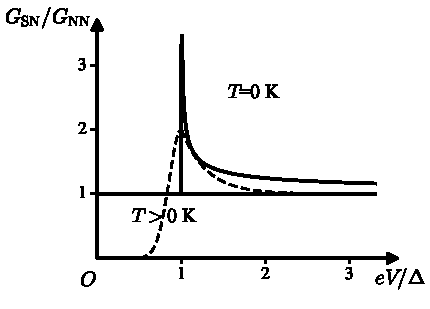
\includegraphics[width=6.5cm]{fig6-13.pdf}\\{\small 图 6.13\quad S-N系统的微分电导}
\end{minipage}
\end{center}

相应的，在低温和小电压情况下隧穿电流之比为
\begin{equation}
  \lim_{\substack{T\to0\\ V\to0}}\frac{I_{\mathrm{SN}}}{I_{\mathrm{NN}}}
  =\left[\frac{2\pi\Delta(0)}{k_{\mathrm{B}}T}\right]^{1/2}
  \mathrm{e}^{-\Delta(0)/k_{\mathrm{B}}T}
\end{equation}
如图6.14中虚线所示，与贾埃弗（Giaever）\textsuperscript{[6]}的实验结果一致（参考图6.3），直接证实了超导体中单个准粒子激发至少需要 $\Delta$ 能量，即存在能隙.

\begin{center}
\begin{minipage}{6cm}
\centering
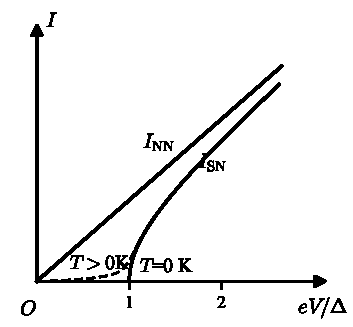
\includegraphics[width=6cm]{fig6-14.pdf}\\{\small 图 6.14\quad $I$-$V$ 曲线}
\end{minipage}
\end{center}

\section{伦敦-皮帕的唯象理论}

超导体的主要特征为：

（i）$T<T_{\mathrm{c}}$ 时直流电阻消失，存在着无阻的超电流，这是超导体的理想导电性.

（ii）迈斯纳效应，弱磁场不能透入大块超导样品内部，表现出完全逆磁性.

在这两个主要特征的基础上，伦敦建立了描述超导体电磁性质的唯象理论，皮帕又进一步将它推广到包含了磁场的非定域情形.

\subsection*{1. 伦敦方程}

正常金属的电阻效应由欧姆定律 $\boldsymbol{j}=\sigma\boldsymbol{E}$ 描述.为了描述超导体的理想导电性和完全逆磁性，应当有新的关系式.伦敦假定超电流 $\boldsymbol{j}_{\mathrm{s}}(\boldsymbol{r})$ 与电磁场的矢量势 $\boldsymbol{A}(\boldsymbol{r})$ 成正比
\begin{equation}
  \boldsymbol{j}_{\mathrm{s}}=-\frac{1}{c\Lambda}\boldsymbol{A}
  \qquad\left(\Lambda=\frac{m}{n_{\mathrm{s}}e^{2}}\right)
\end{equation}
其比例常量为负数.下面将看到，正是这个负号说明超电流的屏蔽作用，从而保证了完全逆磁性.其中 $n_{\mathrm{s}}$ 代表超导电子浓度，当 $T=0$ K时 $n_{\mathrm{s}}=n$，n即传导电子密度.$\boldsymbol{A}$ 满足横场条件 $\nabla\cdot\boldsymbol{A}=0$.式(6.7.1)被称为伦敦方程，它与麦克斯韦（Maxwell）方程组合可说明超导体的电动力学性质.我们只说明式(6.7.1)包含了超导体的两个主要特征.

（i）理想导电性：式(6.7.1)两边对时间取导数，得
\begin{equation}
  \frac{\partial}{\partial t}\left(\Lambda\boldsymbol{j}_{\mathrm{s}}\right)
  =-\frac{1}{c}\frac{\partial\boldsymbol{A}}{\partial t}=\boldsymbol{E}
\end{equation}
式(6.7.2)就是超导电子的无阻运动方程
$\dfrac{\partial}{\partial t}\left(m\boldsymbol{v}_{\mathrm{s}}\right)=e\boldsymbol{E}$
和 $j_{\mathrm{s}}=n_{\mathrm{s}}e\boldsymbol{v}_{\mathrm{s}}$ 的组合.因此，它代表超导体的理想导电性.式(6.7.2)说明当电场 $\boldsymbol{E}=0$ 时，也存在 $\boldsymbol{j}_{\mathrm{s}}=$ 常数的超导持续电流.

（ii）完全逆磁性：对式(6.7.1)两边取旋度，得到方程
\begin{equation}
  \boldsymbol{B}=-c\Lambda\,\nabla\times\boldsymbol{j}_{\mathrm{s}}
\end{equation}
再利用麦克斯韦方程 $\nabla\times\boldsymbol{B}=\dfrac{4\pi}{c}\boldsymbol{j}_{\mathrm{s}}$ 和 $\nabla\cdot\boldsymbol{B}=0$，求得
\begin{equation}
  \nabla^{2}\boldsymbol{B}=\frac{1}{\lambda_{\mathrm{L}}^{2}}\boldsymbol{B}
  \qquad\left(\lambda_{\mathrm{L}}^{2}=\frac{mc^{2}}{4\pi n_{\mathrm{s}}e^{2}}\right)
\end{equation}
对于 $z>0$ 的半无限超导样品，当外磁场平行于 $z=0$ 平面时，式(6.7.3)简化为
\begin{equation}
  \frac{\mathrm{d}^{2}\boldsymbol{B}}{\mathrm{d}z^{2}}
  =\frac{\boldsymbol{B}}{\lambda_{\mathrm{L}}^{2}}
\end{equation}
其指数衰减解为
\begin{equation}
  \boldsymbol{B}(z)=\boldsymbol{B}(0)\exp\left(-z/\lambda_{\mathrm{L}}\right)
\end{equation}
上式说明，只在样品表面内约为 $\lambda_{\mathrm{L}}$ 厚度的薄层内存在磁场，深入到样品内部时 $\boldsymbol{B}$ 已下降到零.对于超电流 $j_{\mathrm{s}}$ 利用式(6.7.3)和麦克斯韦方程同样可求得
\begin{equation}
  \nabla^{2}\boldsymbol{j}_{\mathrm{s}}=\frac{1}{\lambda_{\mathrm{L}}^{2}}\boldsymbol{j}_{\mathrm{s}}
\end{equation}
因此，在恒定磁场中超导电流也分布在表面内 $\lambda_{\mathrm{L}}$ 厚度中，相应的 $\boldsymbol{A}$ 也在 $\lambda_{\mathrm{L}}$ 尺度上降为零.不难验证，$j_{\mathrm{s}}$ 起着屏蔽样品内部磁场的作用.例如，在上述半无限样品中，若设外磁场沿正x轴方向，则根据伦敦方程(6.7.1)，$j_{\mathrm{s}}$ 沿y轴负方向.通过 $\nabla\times\boldsymbol{B}=\dfrac{4\pi}{c}\boldsymbol{j}_{\mathrm{s}}$，可判断超导流 $j_{\mathrm{s}}$ 的磁场取向，它恰好沿x轴负方向，起着屏蔽外磁场的作用，使大块样品内部的磁感应强度 $\boldsymbol{B}=0$，此即迈斯纳效应.所以，伦敦方程也反映了超导体的完全逆磁性. $\lambda_{\mathrm{L}}$ 代表磁场透入超导样品的深度，称为穿透深度，它是超导体的一个重要特征参量.伦敦方程可以用 $\lambda_{\mathrm{L}}$ 表示为
\begin{equation}
  \boldsymbol{j}_{\mathrm{s}}(\boldsymbol{r})
  =-\frac{c}{4\pi}\frac{1}{\lambda_{\mathrm{L}}^{2}}\boldsymbol{A}(\boldsymbol{r})
\end{equation}
式(6.7.8)说明当穿透深度增大时，超电流减小.当 $T=0$ 时
\begin{equation}
  \lambda_{\mathrm{L}}(0)=\left(\frac{mc^{2}}{4\pi ne^{2}}\right)^{\frac{1}{2}}
\end{equation}
对于纯金属超导样品，$\lambda_{\mathrm{L}}(0)$ 约为 $10^{-6}\sim10^{-5}$ cm量级.但是，实验测定值往往比 $\lambda_{\mathrm{L}}(0)$ 大好几倍.这是因为伦敦方程忽略了超导体的另一个重要参量——相干长度 $\xi_{0}$ 的影响.

\subsection*{2. 皮帕公式}

伦敦方程(6.7.1)假定超电流密度 $\boldsymbol{j}_{\mathrm{s}}(\boldsymbol{r})$ 正比于同一点的矢量势 $\boldsymbol{A}(\boldsymbol{r})$，这是一个定域的关系式.但是，超导体中由于在相干长度 $\xi_{0}=\dfrac{\hbar v_{\mathrm{F}}}{\pi\Delta(0)}$ 范围内存在着电子运动的关联，因此作用于某一点的扰动势必将会影响 $\xi_{0}$ 空间尺度内超导电子的运动速度和电流密度.反过来，在空间某一点的超电流密度也必定会受到其邻近 $\xi_{0}$ 尺度内扰动势的影响.这样，$\boldsymbol{j}_{\mathrm{s}}(\boldsymbol{r})$ 不仅决定于同一点的 $\boldsymbol{A}(\boldsymbol{r})$，还应当包括 $|\boldsymbol{r}-\boldsymbol{r}'|<\xi_{0}$ 范围内各点 $\boldsymbol{r}'$ 的矢量势 $\boldsymbol{A}(\boldsymbol{r}')$ 的贡献.为此，皮帕假定 $j_{\mathrm{s}}$ 与A的非定域关系为
\begin{equation}
  \boldsymbol{j}_{\mathrm{s}}(\boldsymbol{r})
  =-\frac{3}{4\pi\xi_{0}\Lambda c}
  \int\frac{\boldsymbol{R}\left[\boldsymbol{R}\cdot\boldsymbol{A}(\boldsymbol{r}')\right]}
  {R^{4}}\,\mathrm{e}^{-R/\xi_{0}}\mathrm{d}\boldsymbol{r}'
  \qquad\left(\boldsymbol{R}=\boldsymbol{r}-\boldsymbol{r}'\right)
\end{equation}
当A在 $\xi_{0}$ 距离上变化缓慢时，A可以从积分号中提出，从而求得定域关系：
\begin{equation}
\begin{aligned}
  \left[j_{\mathrm{s}}(\boldsymbol{r})\right]_{\mu}
  &\approx-\frac{1}{\xi_{0}\Lambda c}\sum_{\nu}A_{\nu}(\boldsymbol{r})
  \frac{3}{4\pi}\int\mathrm{d}^{3}R\,R_{\mu}R_{\nu}\,
  \frac{\mathrm{e}^{-R/\xi_{0}}}{R^{4}}\\
  &=\frac{1}{\Lambda c}\sum_{\nu}A_{\nu}(\boldsymbol{r})\,\delta_{\mu\nu}
  \left[\frac{1}{\xi_{0}}\int_{0}^{R}\mathrm{d}R\,\mathrm{e}^{-R/\xi_{0}}\right]\\
  &=-\frac{1}{\Lambda c}A_{\mu}(\boldsymbol{r})
\end{aligned}
\end{equation}
式(6.7.11)的矢量表示式即伦敦方程.根据“1”中讨论A在穿透深度 $\lambda_{\mathrm{L}}$ 范围内指数衰减为零.因此，伦敦方程只适用于 $\lambda_{\mathrm{L}}\gg\xi_{0}$ 情况，这时在 $\xi_{0}$ 尺度上j与A的变化都很缓慢.但是纯金属的 $\lambda_{\mathrm{L}}\ll\xi_{0}$，显然纯金属中A在 $\xi_{0}$ 尺度上变化很急剧，这时伦敦方程不适用，必须应用皮帕公式(6.7.10)，所算出的超电流 $j_{\mathrm{s}}$ 必然比按照伦敦方程计算的小.由于超电流减小，意味着穿透深度的增大，因此按式(6.7.10)算出的穿透深度 $\lambda_{\text{理}}$ 将比 $\lambda_{\mathrm{L}}(0)$ 大.精确计算的结果列于表6.2中，它与实验测量值基本相符.因此伦敦穿透深度 $\lambda_{\mathrm{L}}$ 与实验值有分歧的原因是忽略了磁场的非定域效应.不仅如此，将皮帕公式推广用于含杂质超导体，也圆满地解释了实验事实\textsuperscript{[7]}.总之，皮帕公式适用于更普遍的情况.在下一节中我们将看到从BCS理论导出的 $j_{\mathrm{s}}$ 和A关系与皮帕公式相近，可认为是伦敦-皮帕唯象理论的微观证明.

\begin{center}
\begin{minipage}{10.5cm}\centering\small
表 6.2\\[0.5em]
\begin{tabular}{lcccc}
\hline
纯金属 & $\lambda_{\mathrm{L}}$/nm & $\xi_{0}$/nm & $\lambda_{\text{理}}$/nm & $\lambda_{\text{实}}$/nm\\
\hline
Al & $157\times10^{-1}$ & $16\,000\times10^{-1}$ & $530\times10^{-1}$ & $(490\sim515)\times10^{-1}$\\
Sn & $355\times10^{-1}$ & $2\,300\times10^{-1}$ & $560\times10^{-1}$ & $510\times10^{-1}$\\
\hline
\end{tabular}
\end{minipage}
\end{center}

为了将在§8中讨论方便起见，在这里先给出伦敦-皮帕公式的傅里叶变换表示式.利用下列变换式：
\begin{equation}
  \left.
  \begin{aligned}
    \boldsymbol{j}(\boldsymbol{q})
    &=\int\mathrm{d}^{3}r\,\mathrm{e}^{-\mathrm{i}\boldsymbol{q}\cdot\boldsymbol{r}}
    \boldsymbol{j}(\boldsymbol{r})\\
    \boldsymbol{A}(\boldsymbol{q})
    &=\int\mathrm{d}^{3}r\,\mathrm{e}^{-\mathrm{i}\boldsymbol{q}\cdot\boldsymbol{r}}
    \boldsymbol{A}(\boldsymbol{r})
  \end{aligned}\right\}
\end{equation}
可立刻求得零温伦敦方程式(6.7.8)的傅里叶变换公式
\begin{equation}
  \boldsymbol{j}(\boldsymbol{q})
  =-\frac{c}{4\pi}K_{\mathrm{L}}(q)\boldsymbol{A}(\boldsymbol{q})
\end{equation}
其中
\begin{equation}
  K_{\mathrm{L}}(q)=K_{\mathrm{L}}(0)=\lambda_{\mathrm{L}}^{-2}(0)
\end{equation}
对于皮帕公式(6.7.10)
\begin{equation}
  \boldsymbol{j}(\boldsymbol{q})=-\frac{c}{4\pi}\frac{1}{\lambda_{\mathrm{L}}^{2}(0)}
  \frac{3}{4\pi\xi_{0}}\int\mathrm{d}^{3}R\,
  \frac{\boldsymbol{R}\left[\boldsymbol{R}\cdot\boldsymbol{A}(\boldsymbol{q})\right]}{R^{4}}\,
  \mathrm{e}^{-R/\xi_{0}}\mathrm{e}^{-\mathrm{i}\boldsymbol{q}\cdot\boldsymbol{R}}
\end{equation}
利用横场条件 $\boldsymbol{q}\cdot\boldsymbol{A}(\boldsymbol{q})=0$（即 $\nabla\cdot\boldsymbol{A}=0$），不难求出
\begin{equation}
  \boldsymbol{j}(\boldsymbol{q})
  =-\frac{c}{4\pi}K(q)\boldsymbol{A}(\boldsymbol{q})
\end{equation}
\begin{equation}
  K(q)=\frac{1}{\lambda_{\mathrm{L}}^{2}(0)\xi_{0}}
  \int_{0}^{\infty}\mathrm{d}R\,\mathrm{e}^{-R/\xi_{0}}
  \left\{\frac{3}{qR}\mathrm{j}_{1}(qR)\right\}
\end{equation}
其中 $\mathrm{j}_{1}$ 为球贝塞尔函数：
\begin{equation}
  \mathrm{j}_{1}(x)=\frac{\sin x}{x^{2}}-\frac{\cos x}{x}
\end{equation}
皮帕的 $K(q)$ 如图6.15所示.在两个极限情况下的 $K(q)$ 分别为

\begin{center}
\begin{minipage}{5.5cm}
\centering
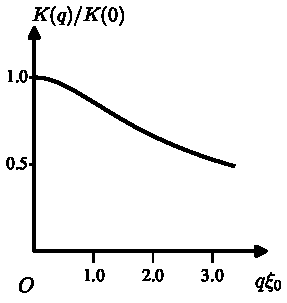
\includegraphics[width=5.5cm]{fig6-15.pdf}\\{\small 图 6.15\quad 皮帕的 $K(q)$}
\end{minipage}
\end{center}

（i）$q\xi_{0}\ll1$，积分式(6.7.17)主要贡献在 $qR=0$ 处，考虑到 $\left\{\dfrac{3}{qR}\mathrm{j}_{1}(qR)\right\}$ 相对于指数因子为缓变函数，可取
\begin{equation*}
  \lim_{qR\to0}\left\{\frac{3}{qR}\mathrm{j}_{1}(qR)\right\}=1
\end{equation*}
则
\begin{equation}
\begin{aligned}
  K(q)\approx K(0)&=\frac{1}{\lambda_{\mathrm{L}}^{2}(0)}
  \left\{\frac{1}{\xi_{0}}\int_{0}^{\infty}\mathrm{d}R\,\mathrm{e}^{-R/\xi_{0}}\right\}
  =\frac{1}{\lambda_{\mathrm{L}}^{2}(0)}\\
  &=K_{\mathrm{L}}(0)\qquad(q\xi_{0}\ll1)
\end{aligned}
\end{equation}
（ii）$q\xi_{0}\gg1$：将式(6.7.17)中指数因子近似用1代替，求出
\begin{equation}
\begin{aligned}
  K(q)&\approx\frac{1}{\lambda_{\mathrm{L}}^{2}(0)}
  \left(\frac{1}{q\xi_{0}}\right)\int_{0}^{\infty}\frac{3}{x}\mathrm{j}_{1}(x)\,\mathrm{d}x\\
  &=K(0)\frac{3\pi}{4q\xi_{0}}\qquad(q\xi_{0}\gg1)
\end{aligned}
\end{equation}

\section{迈斯纳效应}

我们将从BCS理论出发研究超导体在弱磁场中的行为，它属于超导体与电磁场互作用的静态 $\left(\omega=0\right)$ 极限情况.根据§7中的讨论可知，如果在 $q\to0$ 时求得的公式
$\boldsymbol{j}(\boldsymbol{q})=-\dfrac{c}{4\pi}\boldsymbol{K}(q)\boldsymbol{A}(\boldsymbol{q})$
中 $K(0)>0$，就表示有迈斯纳效应，若 $K(0)=0$，则无迈斯纳效应.此外，在本节中我们还要从微观角度证明超电流与矢量势的非定域关系.为简单起见仅讨论 $T=0$ K情况.

\subsection*{1. 互作用哈密顿量H}

互作用项 $H_{1}$ 由外场中动能的增量决定，在弱磁场作用下，准至A的线性项时得
\begin{equation}
  \frac{1}{2m}\left(\hat{\boldsymbol{p}}-\frac{e}{c}\boldsymbol{A}\right)^{2}
  -\frac{1}{2m}\hat{\boldsymbol{p}}^{2}
  \approx\frac{\mathrm{i}e\hbar}{2mc}
  \left(\boldsymbol{A}\cdot\nabla+\nabla\cdot\boldsymbol{A}\right)
\end{equation}
$H_{1}$ 的二次量子化表示式为
\begin{equation}
  H_{1}=\frac{\mathrm{i}e\hbar}{2mc}\int
  \Psi^{+}\left(\boldsymbol{A}\cdot\nabla+\nabla\cdot\boldsymbol{A}\right)
  \Psi\,\mathrm{d}\boldsymbol{r}
\end{equation}
按傅里叶级数展开矢量势，得
\begin{equation}
  \boldsymbol{A}(\boldsymbol{r})=\sum_{\boldsymbol{q}}
  \boldsymbol{A}(\boldsymbol{q})\,\mathrm{e}^{\mathrm{i}\boldsymbol{q}\cdot\boldsymbol{r}}
\end{equation}
将 $\Psi$ 按平面波展开，设样品取单位体积时
\begin{equation}
  \Psi(\boldsymbol{r})=\sum_{k,\,\sigma}C_{k\sigma}\,
  \mathrm{e}^{\mathrm{i}\boldsymbol{k}\cdot\boldsymbol{r}}\chi_{\sigma}
\end{equation}
当 $\sigma=\pm1$ 时，$\chi_{\sigma}$ 分别为 $\binom{1}{0}$ 和 $\binom{0}{1}$，$\chi_{\sigma}$ 满足关系
\begin{equation}
  \chi^{+}_{\sigma'}\chi_{\sigma}=\delta_{\sigma'\sigma}
\end{equation}
因此
\begin{equation}
\begin{aligned}
  H_{1}&=-\frac{e\hbar}{2mc}\sum_{k,\,k',\,q,\,\sigma}
  C^{+}_{k'\sigma}C_{k\sigma}\left(2\boldsymbol{k}+\boldsymbol{q}\right)
  \cdot\boldsymbol{A}(\boldsymbol{q})
  \int\mathrm{e}^{\mathrm{i}\left(\boldsymbol{k}+\boldsymbol{q}-\boldsymbol{k}'\right)
  \cdot\boldsymbol{r}}\mathrm{d}\boldsymbol{r}\\
  &=-\frac{e\hbar}{2mc}\sum_{k,\,q,\,\sigma}
  \left(2\boldsymbol{k}+\boldsymbol{q}\right)\cdot\boldsymbol{A}(\boldsymbol{q})\,
  C^{+}_{k+q,\,\sigma}C_{k\sigma}
\end{aligned}
\end{equation}
磁场矢量势采用横场规范 $\boldsymbol{q}\cdot\boldsymbol{A}(\boldsymbol{q})=0$，并根据§2中约定记 $(\boldsymbol{k},\uparrow)$ 为k，记 $(-\boldsymbol{k},\downarrow)$ 为$-k$，可将式(6.8.6)改写成
\begin{equation}
  H_{1}=-\frac{e\hbar}{mc}\sum_{k,\,q}
  \left[\boldsymbol{k}\cdot\boldsymbol{A}(\boldsymbol{q})\right]
  \left(C^{+}_{k+q}C_{k}-C^{+}_{-k}C_{-k-q}\right)
\end{equation}
再利用式(6.4.15)，将 $H_{1}$ 用超导元激发算符 $\alpha$、$\alpha^{+}$ 表示：
\begin{equation}
\begin{aligned}
  H_{1}=-\frac{e\hbar}{mc}\sum_{k,\,q}
  \left[\boldsymbol{k}\cdot\boldsymbol{A}(\boldsymbol{q})\right]
  &\left[\left(u_{k+q}v_{k}-u_{k}v_{k+q}\right)
  \left(\alpha^{+}_{k+q}\alpha^{+}_{-k}
  +\alpha_{k}\alpha_{-k-q}\right)\right.\\
  \left.+\left(u_{k+q}u_{k}+v_{k+q}v_{k}\right)
  \left(\alpha^{+}_{k+q}\alpha_{k}
  -\alpha^{+}_{-k}\alpha_{-k-q}\right)\right]
\end{aligned}
\end{equation}

\subsection*{2. 电流密度算符}

根据量子力学，电磁场中电流密度算符可由连续性方程导出，其二次量子化表示为
\begin{equation}
\begin{aligned}
  \hat{\boldsymbol{j}}(\boldsymbol{r})
  &=\frac{e\hbar}{2m\mathrm{i}}\left[\Psi^{+}\left(\nabla\Psi\right)
  -\left(\nabla\Psi^{+}\right)\Psi\right]
  -\frac{e^{2}}{mc}\Psi^{+}\boldsymbol{A}\Psi\\
  &\equiv\hat{\boldsymbol{j}}_{1}(\boldsymbol{r})+\hat{\boldsymbol{j}}_{2}(\boldsymbol{r})
\end{aligned}
\end{equation}
其中
\begin{equation}
\begin{aligned}
  \hat{\boldsymbol{j}}_{1}(\boldsymbol{r})
  &\equiv\frac{e\hbar}{2m\mathrm{i}}\left[\Psi^{+}\left(\nabla\Psi\right)
  -\left(\nabla\Psi^{+}\right)\Psi\right]\\
  &=\frac{e\hbar}{2m}\sum_{k,\,q}\left(2\boldsymbol{k}+\boldsymbol{q}\right)
  \mathrm{e}^{-\mathrm{i}\boldsymbol{q}\cdot\boldsymbol{r}}
  \left(C^{+}_{k+q}C_{k}-C^{+}_{-k}C_{-k-q}\right)
\end{aligned}
\end{equation}
\begin{equation}
\begin{aligned}
  \hat{\boldsymbol{j}}_{2}(\boldsymbol{r})
  &\equiv-\frac{e^{2}}{mc}\Psi^{+}\boldsymbol{A}\Psi\\
  &=-\frac{e^{2}}{mc}\boldsymbol{A}(\boldsymbol{r})\sum_{k,\,q}
  \mathrm{e}^{-\mathrm{i}\boldsymbol{q}\cdot\boldsymbol{r}}
  \left(C^{+}_{k+q}C_{k}+C^{+}_{-k}C_{-k-q}\right)
\end{aligned}
\end{equation}
这里已采用了与式(6.8.7)相同的约定符号.

式(6.8.11)中的负号说明它代表逆磁电流部分.在弱磁场作用下，只需计算到A的一阶，这时可用零场时的超导基态 $|0\rangle_{0}$ 对 $\hat{j}_{2}$ 求平均，得到 $T=0$ K时的电流响应
\begin{equation*}
\begin{aligned}
  \boldsymbol{j}_{2}(\boldsymbol{r})
  &\equiv\langle\hat{\boldsymbol{j}}_{2}(\boldsymbol{r})\rangle_{0}\\
  &=-\frac{e^{2}}{mc}\boldsymbol{A}(\boldsymbol{r})\sum_{k,\,q}
  \mathrm{e}^{-\mathrm{i}\boldsymbol{q}\cdot\boldsymbol{r}}
  \,_{0}\langle0|\left(C^{+}_{k+q}C_{k}+C^{+}_{-k}C_{-k-q}\right)|0\rangle_{0}
\end{aligned}
\end{equation*}
上式中，只有 $q=0$ 项有贡献，并且 $_{0}\langle0|C^{+}_{k}C_{k}|0\rangle_{0}=v_{k}^{2}
=\,_{0}\langle0|C^{+}_{-k}C_{-k}|0\rangle_{0}$，这时
\begin{equation*}
  \boldsymbol{j}_{2}(\boldsymbol{r})=-\frac{e^{2}}{mc}\boldsymbol{A}(\boldsymbol{r})
  \sum_{k}2v_{k}^{2}
  =-\frac{e^{2}}{mc}\boldsymbol{A}(\boldsymbol{r})
  \sum_{k}\left(1-\frac{\varepsilon_{k}}{\xi_{k}}\right)
\end{equation*}
上式右边第二项是 $\varepsilon_{k}$ 的奇函数，它对 $j_{2}$ 无贡献.另外，在样品取单位体积时，应有 $\sum_{k}1=n$，代表传导电子密度.因此
\begin{equation}
  \boldsymbol{j}_{2}(\boldsymbol{r})=\frac{ne^{2}}{mc}\boldsymbol{A}(\boldsymbol{r})
  =-\frac{c}{4\pi}\lambda_{\mathrm{L}}^{-2}(0)\boldsymbol{A}(\boldsymbol{r})
\end{equation}
即伦敦方程(6.7.8).读者不难自行验证，式(6.8.12)的结果对于正常态和超导态是一样的.因此，证明迈斯纳效应的关键在于对 $\boldsymbol{j}_{1}(\boldsymbol{r})$ 的计算.$\hat{j}_{1}$ 的元激发算符表示式为
\begin{equation}
\begin{aligned}
  \hat{\boldsymbol{j}}_{1}(\boldsymbol{r})
  =\frac{e\hbar}{2m}\sum_{k,\,q}&\left(2\boldsymbol{k}+\boldsymbol{q}\right)
  \mathrm{e}^{-\mathrm{i}\boldsymbol{q}\cdot\boldsymbol{r}}
  \left\{\left(u_{k+q}v_{k}-u_{k}v_{k+q}\right)
  \left(\alpha^{+}_{k+q}\alpha^{+}_{-k}
  +\alpha_{k}\alpha_{-k-q}\right)\right.\\
  &+\left.\left(u_{k+q}u_{k}+v_{k+q}v_{k}\right)
  \left(\alpha^{+}_{k+q}\alpha_{k}
  -\alpha^{+}_{-k}\alpha_{-k-q}\right)\right\}
\end{aligned}
\end{equation}

\subsection*{3. 弱磁场中的电流响应}

计算 $\hat{j}_{1}$ 时，应当考虑A对超导态的影响，利用微扰论，准至A一阶的状态为
\begin{equation}
  |0\rangle_{1}=|0\rangle_{0}
  +{\sum_{l}}'\,|l\rangle_{0}\,
  \frac{_{0}\langle l|H_{1}|0\rangle_{0}}{E_{0}-E_{l}}
\end{equation}
而
\begin{equation}
\begin{aligned}
  \boldsymbol{j}_{1}(\boldsymbol{r})
  ={}_{0}\langle0|\hat{j}_{1}|0\rangle_{0}
  +{\sum_{l}}'\biggl\{&\frac{_{0}\langle0|\hat{j}_{1}|l\rangle_{0}\,
  _{0}\langle l|H_{1}|0\rangle_{0}}{E_{0}-E_{l}}\\
  +&\frac{_{0}\langle0|H_{1}|l\rangle_{0}\,
  _{0}\langle l|\hat{j}_{1}|0\rangle_{0}}{E_{0}-E_{l}}\biggr\}+\cdots
\end{aligned}
\end{equation}
从式(6.8.8)和(6.8.13)可以看出 $\hat{j}_{1}$ 与 $H_{1}$ 中只有 $\alpha^{+}_{k+q}\alpha^{+}_{-k}$ 对基态作用不等于零，故中间态 $|l\rangle_{0}$ 取为
\begin{equation}
  |l\rangle_{0}=\alpha^{+}_{k+q}\alpha^{+}_{-k}|0\rangle\text{；}
  \qquad E_{0}=0\text{；}\qquad E_{l}=\xi_{k+q}+\xi_{k}
\end{equation}
由此算出矩阵元
\begin{equation}
\begin{aligned}
  &_{0}\langle l|H_{1}|0\rangle_{0}
  =-\frac{e\hbar}{mc}\left[\boldsymbol{k}\cdot\boldsymbol{A}(\boldsymbol{q})\right]
  \left(u_{k+q}v_{k}-u_{k}v_{k+q}\right)\\
  &_{0}\langle l|\hat{j}_{1}|0\rangle_{0}
  =\frac{e\hbar}{2m}\left[\left(2\boldsymbol{k}+\boldsymbol{q}\right)
  \mathrm{e}^{-\mathrm{i}\boldsymbol{q}\cdot\boldsymbol{r}}\right]
  \left(u_{k+q}v_{k}-u_{k}v_{k+q}\right)
\end{aligned}
\end{equation}
\begin{equation}
\begin{aligned}
  &_{0}\langle0|\hat{j}_{1}|l\rangle_{0}
  =\frac{e\hbar}{2m}\left[\left(2\boldsymbol{k}+\boldsymbol{q}\right)
  \mathrm{e}^{\mathrm{i}\boldsymbol{q}\cdot\boldsymbol{r}}\right]
  \left(u_{k+q}v_{k}-u_{k}v_{k+q}\right)\\
  &_{0}\langle0|H_{1}|l\rangle_{0}
  =-\frac{e\hbar}{mc}\left[\boldsymbol{k}\cdot\boldsymbol{A}(-\boldsymbol{q})\right]
  \left(u_{k+q}v_{k}-u_{k}v_{k+q}\right)\\
  &_{0}\langle0|\hat{j}_{1}|0\rangle_{0}=0
\end{aligned}
\end{equation}
代入式(6.8.15)中，经整理得到
\begin{equation}
  \boldsymbol{j}_{1}(\boldsymbol{r})
  =\left(\frac{e\hbar}{m}\right)^{2}\frac{1}{c}\sum_{k,\,q}
  \left(u_{k+q}v_{k}-u_{k}v_{k+q}\right)^{2}
  \frac{\left(2\boldsymbol{k}+\boldsymbol{q}\right)
  \left[\boldsymbol{k}\cdot\boldsymbol{A}(\boldsymbol{q})\right]}
  {\xi_{k}+\xi_{k+q}}\,\mathrm{e}^{\mathrm{i}\boldsymbol{q}\cdot\boldsymbol{r}}
\end{equation}
其中u、v由式(6.4.20)决定，$\xi_{k}=\sqrt{\varepsilon_{k}^{2}+\Delta^{2}}$.对上式作变数代换 $\boldsymbol{k}\to\boldsymbol{k}-\dfrac{\boldsymbol{q}}{2}$，则 $j_{1}$ 的傅里叶变换可写为下列对称形式：
\begin{equation}
  \boldsymbol{j}_{1}(\boldsymbol{q})
  =2\frac{e^{2}\hbar^{2}}{m^{2}c}\sum_{k}
  \frac{\boldsymbol{k}\left[\boldsymbol{k}\cdot\boldsymbol{A}(\boldsymbol{q})\right]}
  {\xi_{k-\frac{q}{2}}+\xi_{k+\frac{q}{2}}}
  \left(u_{k+\frac{q}{2}}v_{k-\frac{q}{2}}
  -u_{k-\frac{q}{2}}v_{k+\frac{q}{2}}\right)^{2}
\end{equation}
将求和化为积分，取 $\boldsymbol{q}$ 为极轴，注意到 $\boldsymbol{q}\perp\boldsymbol{A}(\boldsymbol{q})$［因为 $\boldsymbol{A}(\boldsymbol{q})\cdot\boldsymbol{q}=0$］，并设 $\theta$ 为 $\boldsymbol{k}$ 与 $\boldsymbol{q}$ 之夹角，则积分只有沿 $\boldsymbol{A}(\boldsymbol{q})$ 方向的分量
\begin{equation*}
\begin{aligned}
  \boldsymbol{j}_{1}(\boldsymbol{q})
  =2\frac{e^{2}\hbar^{2}}{m^{2}c}\frac{1}{(2\pi)^{3}}
  &\int_{0}^{2\pi}\cos^{2}\phi\,\mathrm{d}\phi
  \int_{-1}^{+1}\sin^{2}\theta\,\mathrm{d}\cos\theta
  \int_{0}^{\infty}k^{4}\mathrm{d}k\,\times\\
  &\frac{\left(u_{k+\frac{q}{2}}v_{k-\frac{q}{2}}
  -u_{k-\frac{q}{2}}v_{k+\frac{q}{2}}\right)^{2}}
  {\xi_{k+\frac{q}{2}}+\xi_{k-\frac{q}{2}}}\boldsymbol{A}(\boldsymbol{q})
\end{aligned}
\end{equation*}
为简化符号起见，定义
\begin{equation}
\begin{aligned}
  &\varepsilon_{\pm}\equiv\varepsilon_{k\pm q/2}\text{，}
  \qquad\xi_{\pm}\equiv\xi_{k\pm q/2}
  =\sqrt{\varepsilon_{\pm}^{2}+\Delta^{2}}\\
  &u_{\pm}\equiv u_{k\pm q/2}\text{，}
  \qquad v_{\pm}\equiv v_{k\pm q/2}\text{，}
  \qquad Z\equiv\cos\theta
\end{aligned}
\end{equation}
将 $\boldsymbol{j}_{1}(\boldsymbol{q})$ 写成
\begin{equation*}
\begin{aligned}
  \boldsymbol{j}_{1}(\boldsymbol{q})
  =\frac{2e^{2}\hbar^{2}}{m^{2}c}\frac{1}{(2\pi)^{3}}
  &\int_{0}^{2\pi}\cos^{2}\phi\,\mathrm{d}\phi
  \left\{\int_{-1}^{1}\left(1-Z^{2}\right)\mathrm{d}Z\,\times\right.\\
  &\left.\int_{0}^{\infty}k^{4}\mathrm{d}k
  \left\{\frac{\left(u_{+}v_{-}-u_{-}v_{+}\right)^{2}}
  {\xi_{+}+\xi_{-}}\right\}\boldsymbol{A}(\boldsymbol{q})\right\}\\
  \approx\frac{2e^{2}\hbar}{mc}\frac{1}{(2\pi)^{3}}\pi k_{\mathrm{F}}^{3}
  &\int_{-1}^{1}\left(1-Z^{2}\right)\mathrm{d}Z\,\times\\
  &\int_{-\infty}^{\infty}\mathrm{d}\varepsilon
  \left\{\frac{\left(u_{+}v_{-}-u_{-}v_{+}\right)^{2}}
  {\xi_{+}+\xi_{-}}\right\}\boldsymbol{A}(\boldsymbol{q})
\end{aligned}
\end{equation*}
上式中 $\varepsilon$ 是从费密面 $E_{\mathrm{F}}$ 算起的能量，$\{\cdots\}$ 只是 $\varepsilon$ 和Z的函数，与 $\phi$ 无关.根据式(6.4.19)和(6.4.20)容易导出
\begin{equation}
  \left(u_{+}v_{-}-u_{-}v_{+}\right)^{2}
  =\frac{1}{2}\left\{\frac{\xi_{+}\xi_{-}
  -\varepsilon_{+}\varepsilon_{-}-\Delta^{2}}{\xi_{+}\xi_{-}}\right\}
\end{equation}
再利用 $\dfrac{k_{\mathrm{F}}^{3}}{3\pi^{2}}=n$，可将 $\boldsymbol{j}_{1}(\boldsymbol{q})$ 整理成标准形式
\begin{equation}
\begin{aligned}
  \boldsymbol{j}_{1}(\boldsymbol{q})
  &=-\frac{c}{4\pi}\frac{\boldsymbol{A}(\boldsymbol{q})}{\lambda_{\mathrm{L}}^{2}(0)}
  \left(-\frac{3}{4}\right)\int_{-1}^{+1}\left(1-Z^{2}\right)\mathrm{d}Z\,\times\\
  &\quad\int_{-\infty}^{\infty}\mathrm{d}\varepsilon\,
  \frac{1}{2}\frac{\xi_{+}\xi_{-}-\varepsilon_{+}\varepsilon_{-}-\Delta^{2}}
  {\xi_{+}\xi_{-}\left(\xi_{+}+\xi_{-}\right)}
\end{aligned}
\end{equation}
逆磁电流密度 $\boldsymbol{j}_{2}(\boldsymbol{q})$ 根据式(6.8.12)决定.这样，总电流密度的傅里叶变换为
\begin{equation}
\begin{aligned}
  \boldsymbol{j}(\boldsymbol{q})&=-\frac{c}{4\pi}K(q)\boldsymbol{A}(\boldsymbol{q})\\
  K(q)&=\frac{1}{\lambda_{\mathrm{L}}^{2}(0)}\left\{1-\frac{3}{4}
  \int_{-1}^{+1}\left(1-Z^{2}\right)\mathrm{d}Z\,\times
  \int_{-\infty}^{\infty}\mathrm{d}\varepsilon\,
  \frac{1}{2}\frac{\xi_{+}\xi_{-}-\varepsilon_{+}\varepsilon_{-}-\Delta^{2}}
  {\xi_{+}\xi_{-}\left(\xi_{+}+\xi_{-}\right)}\right\}
\end{aligned}
\end{equation}
其中 $K(q)$ 与取向无关，而
\begin{equation}
  \varepsilon_{\pm}\approx\varepsilon\pm\frac{1}{2}\hbar qv_{\mathrm{F}}Z\text{，}
  \qquad \varepsilon_{+}-\varepsilon_{-}=\hbar qv_{\mathrm{F}}Z
\end{equation}
略去的项为 $\dfrac{q}{k_{\mathrm{F}}}$ 量级.注意，在今后的讨论中无论 $q\xi_{0}\ll1$ 或 $q\xi_{0}\gg1$ 情况，q都满足限制 $q\ll k_{\mathrm{F}}$.因此，穿透深度总比原子间距大很多.

\subsection*{4. $K(q)$的计算}

首先证明正常导体 $K_{\mathrm{n}}(q)=0$，无迈斯纳效应，因为正常导体 $\Delta=0$，$\xi_{\pm}=|\varepsilon_{\pm}|$，式(6.8.24)简化为
\begin{equation}
\begin{aligned}
  K_{\mathrm{n}}(q)
  &=\frac{1}{\lambda_{\mathrm{L}}^{2}(0)}\biggl\{1-\frac{3}{4}
  \int_{-1}^{1}\left(1-Z^{2}\right)\mathrm{d}Z\,\times\\
  &\quad\int_{-\infty}^{\infty}\mathrm{d}\varepsilon\,
  \frac{1}{2}\left[\frac{|\varepsilon_{+}||\varepsilon_{-}|
  -\varepsilon_{+}\varepsilon_{-}}{|\varepsilon_{+}||\varepsilon_{-}|}\right]
  \frac{1}{|\varepsilon_{+}|+|\varepsilon_{-}|}\biggr\}
\end{aligned}
\end{equation}
当 $\varepsilon_{+}$ 与 $\varepsilon_{-}$ 同号时 $\dfrac{1}{2}\left[\cdots\right]=0$，异号时 $\dfrac{1}{2}\left[\cdots\right]=1$，积分得
\begin{equation}
\begin{aligned}
  &\int_{-\infty}^{\infty}\mathrm{d}\varepsilon\,
  \frac{1}{2}\left[\frac{|\varepsilon_{+}||\varepsilon_{-}|
  -\varepsilon_{+}\varepsilon_{-}}{|\varepsilon_{+}||\varepsilon_{-}|}\right]
  \frac{1}{|\varepsilon_{+}|+|\varepsilon_{-}|}\\
  &\qquad\approx\int_{-\frac{1}{2}\hbar qv_{\mathrm{F}}Z}
  ^{\frac{1}{2}\hbar qv_{\mathrm{F}}Z}
  \frac{\mathrm{d}\varepsilon}{\varepsilon_{+}-\varepsilon_{-}}=1
\end{aligned}
\end{equation}
其中利用了式(6.8.25).上式相当于
\begin{equation*}
  \int_{-\infty}^{\infty}\frac{\mathrm{d}\varepsilon}{\varepsilon_{+}-\varepsilon_{-}}
  \left[\theta(\varepsilon_{+})-\theta(\varepsilon_{-})\right]=1
\end{equation*}
因此
\begin{equation}
  K_{\mathrm{n}}(q)=\frac{1}{\lambda_{\mathrm{L}}^{2}(0)}
  \left\{1-\frac{3}{4}\int_{-1}^{1}\left(1-Z^{2}\right)\mathrm{d}Z\right\}=0
\end{equation}
在正常导体中 $j_{1}$ 与 $j_{2}$ 相互抵消，说明 $j_{1}$ 代表顺磁电流.

对于超导体 $\Delta\neq0$，$K(q)$ 一般应作数值计算.下面仅讨论两个极限情况：

（i）$q\xi_{0}\ll1$ 的情况
\begin{equation*}
  \xi_{0}=\frac{\hbar v_{\mathrm{F}}}{\pi\Delta(0)}
\end{equation*}
属于 $q\to0$ 情况.从 $K(q)$ 公式(6.8.24)可看出，当 $q\to0$ 时 $\varepsilon_{\pm}\to\varepsilon$，$\xi_{\pm}\to\xi$，$K(q)$ 公式中积分项趋于零，因此
\begin{equation}
  K(q)\to\frac{1}{\lambda_{\mathrm{L}}^{2}(0)}=K_{\mathrm{L}}(0)
\end{equation}
这时我们得到伦敦极限情况，说明超导体有迈斯纳效应.具体展开 $\varepsilon_{\pm}$，可估计出 $K(q)$ 中积分项按 $\left(q\xi_{0}\right)^{2}$ 趋于零.由于顺磁电流 $j_{1}$ 趋于零，只剩下逆磁电流项 $j_{2}$，这就证明了唯象理论的式(6.7.19).

（ii）$q\xi_{0}\gg1$ 的情况

这时 $\hbar qv_{\mathrm{F}}\gg\pi\Delta(0)$，下面的计算将证明 $j_{1}$ 与 $j_{2}$ 的主要部分相消.剩余部分正比于 $\left(\dfrac{1}{q\xi_{0}}\right)$，$K(q)$ 仍然大于零.由于 $K_{\mathrm{n}}(q)=0$，可以从 $K(q)-K_{\mathrm{n}}(q)$ 入手，首先消去式(6.8.24)右边第一项，得
\begin{equation}
\begin{aligned}
  K(q)&\equiv K(q)-K_{\mathrm{n}}(q)\\
  &=-\frac{1}{\lambda_{\mathrm{L}}^{2}(0)}\frac{3}{8}
  \int_{-1}^{1}\mathrm{d}Z\left(1-Z^{2}\right)
  \int_{-\infty}^{\infty}\mathrm{d}\varepsilon
  \left\{\frac{1}{\xi_{+}+\xi_{-}}
  \left[1-\frac{\varepsilon_{+}\varepsilon_{-}+\Delta^{2}}{\xi_{+}\xi_{-}}\right]\right.\\
  &\quad\left.-\frac{1}{\varepsilon_{+}-\varepsilon_{-}}
  \left[\left(2\theta(\varepsilon_{+})-1\right)
  -\left(2\theta(\varepsilon_{-})-1\right)\right]\right\}
\end{aligned}
\end{equation}
其中，根据式(6.8.27)—(6.8.28)的讨论，将正常态的 $K_{\mathrm{n}}(q)$ 写成
\begin{equation*}
\begin{aligned}
  K_{\mathrm{n}}(q)&=\frac{1}{\lambda_{\mathrm{L}}^{2}(0)}\biggl\{1-\frac{3}{4}
  \int_{-1}^{1}\mathrm{d}Z\left(1-Z^{2}\right)
  \int_{-\infty}^{\infty}\frac{\mathrm{d}\varepsilon}{\varepsilon_{+}-\varepsilon_{-}}
  \left[\theta(\varepsilon_{+})-\theta(\varepsilon_{-})\right]\biggr\}\\
  &=\frac{1}{\lambda_{\mathrm{L}}^{2}(0)}\biggl\{1-\frac{3}{8}
  \int_{-1}^{1}\mathrm{d}Z\left(1-Z^{2}\right)
  \int_{-\infty}^{\infty}\frac{\mathrm{d}\varepsilon}{\varepsilon_{+}-\varepsilon_{-}}\times\\
  &\quad\left.\left[\left(2\theta(\varepsilon_{+})-1\right)
  -\left(2\theta(\varepsilon_{-})-1\right)\right]\right\}
\end{aligned}
\end{equation*}
再利用 $\xi_{+}^{2}-\xi_{-}^{2}=\varepsilon_{+}^{2}-\varepsilon_{-}^{2}$，导出等式
\begin{equation}
\begin{aligned}
  \frac{1}{\xi_{+}+\xi_{-}}
  &\left[1-\frac{\varepsilon_{+}\varepsilon_{-}+\Delta^{2}}{\xi_{+}\xi_{-}}\right]\\
  &=\frac{2\Delta^{2}}{\varepsilon_{+}^{2}-\varepsilon_{-}^{2}}
  \left(\frac{1}{\xi_{+}}-\frac{1}{\xi_{-}}\right)
  +\frac{1}{\varepsilon_{+}-\varepsilon_{-}}
  \left(\frac{\varepsilon_{+}}{\xi_{+}}-\frac{\varepsilon_{-}}{\xi_{-}}\right)
\end{aligned}
\end{equation}
将式(6.8.30)改写为
\begin{equation}
\begin{aligned}
  K(q)=-\frac{1}{\lambda_{\mathrm{L}}^{2}(0)}\frac{3}{8}
  \int_{-1}^{1}\mathrm{d}Z\left(1-Z^{2}\right)
  \int_{-\infty}^{\infty}\mathrm{d}\varepsilon
  &\left\{\frac{2\Delta^{2}}{\varepsilon_{+}^{2}-\varepsilon_{-}^{2}}
  \left(\frac{1}{\xi_{+}}-\frac{1}{\xi_{-}}\right)\right.\\
  +\frac{1}{\varepsilon_{+}-\varepsilon_{-}}
  &\left[\frac{\varepsilon_{+}}{\xi_{+}}-\left(2\theta(\varepsilon_{+})-1\right)\right]
  -\frac{1}{\varepsilon_{+}-\varepsilon_{-}}
  \left[\frac{\varepsilon_{-}}{\xi_{-}}-\left(2\theta(\varepsilon_{-})-1\right)\right]
  \left.\right\}
\end{aligned}
\end{equation}
由于 $\varepsilon_{+}-\varepsilon_{-}=\hbar qv_{\mathrm{F}}Z$ 与 $\varepsilon$ 无关，因此式(6.8.32)右边第二、三项对 $\varepsilon$ 积分可表示为
\begin{equation*}
  \int_{-\infty}^{\infty}\mathrm{d}\varepsilon
  \left\{\frac{\varepsilon_{\pm}}{|\xi_{\pm}|}
  -\left[2\theta(\varepsilon_{\pm})-1\right]\right\}
\end{equation*}
当 $|\varepsilon|\to\infty$ 时被积函数是绝对收敛的，可将上式变为
\begin{equation*}
  \int_{-\infty}^{\infty}\mathrm{d}\varepsilon_{\pm}
  \left\{\frac{\varepsilon_{\pm}}{|\xi_{\pm}|}
  -\left[2\theta(\varepsilon_{\pm})-1\right]\right\}=0
\end{equation*}
其中考虑$\left[\cdots\right]$是 $\varepsilon_{\pm}$ 的奇函数，所以积分等于零.这样式(6.8.32)简化为
\begin{equation}
\begin{aligned}
  K(q)&=-\frac{3\Delta^{2}}{4\lambda_{\mathrm{L}}^{2}(0)}
  \int_{-1}^{1}\left(1-Z^{2}\right)\mathrm{d}Z
  \int_{-\infty}^{\infty}\mathrm{d}\varepsilon\,
  \frac{\mathrm{d}\varepsilon}{\varepsilon_{+}^{2}-\varepsilon_{-}^{2}}
  \left(\frac{1}{\xi_{+}}-\frac{1}{\xi_{-}}\right)\\
  &=-\frac{3\Delta^{2}}{8\lambda_{\mathrm{L}}^{2}(0)}\frac{1}{\hbar qv_{\mathrm{F}}}
  \int_{-1}^{1}\frac{\left(1-Z^{2}\right)}{Z}\mathrm{d}Z\,\times\\
  &\quad\int_{-\infty}^{\infty}\frac{\mathrm{d}\varepsilon}{\varepsilon}
  \left\{\frac{1}{\left[\left(\varepsilon+\frac{1}{2}\zeta\right)^{2}
  +\Delta^{2}\right]^{1/2}}
  -\frac{1}{\left[\left(\varepsilon-\frac{1}{2}\zeta\right)^{2}
  +\Delta^{2}\right]^{1/2}}\right\}
\end{aligned}
\end{equation}
其中
\begin{equation}
  \zeta\equiv\hbar qv_{\mathrm{F}}Z
\end{equation}
由于积分式(6.8.33)的主要贡献在 $Z=0$，$\varepsilon=0$ 处，可以将缓变因子 $\left(1-Z^{2}\right)$ 用1代替.再将积分变量Z换为 $\zeta$.考虑到 $q\xi_{0}\gg1$，对 $\zeta$ 的积分限可外推至 $\pm\infty$，因此有
\begin{equation}
\begin{aligned}
  K(q)&\approx\frac{3\Delta}{4\pi\lambda_{\mathrm{L}}^{2}(0)}
  \left(\frac{1}{q\xi_{0}}\right)\int_{-\infty}^{\infty}\frac{\mathrm{d}\zeta}{\zeta}
  \int_{0}^{\infty}\frac{\mathrm{d}\varepsilon}{\varepsilon}\,\times\\
  &\quad\left\{\frac{1}{\left[\left(\varepsilon+\frac{1}{2}\zeta\right)^{2}
  +\Delta^{2}\right]^{1/2}}
  -\frac{1}{\left[\left(\varepsilon-\frac{1}{2}\zeta\right)^{2}
  +\Delta^{2}\right]^{1/2}}\right\}\\
  &=-\frac{3\Delta}{4\pi\lambda_{\mathrm{L}}^{2}(0)}
  \left(\frac{1}{q\xi_{0}}\right)\int_{-\infty}^{\infty}
  \frac{\mathrm{d}\varepsilon}{\varepsilon}
  \left\{-4\frac{\operatorname{arsinh}\left(\dfrac{\varepsilon}{\Delta}\right)}
  {\sqrt{\varepsilon^{2}+\Delta^{2}}}\right\}
\end{aligned}
\end{equation}
令 $x\equiv\operatorname{arsinh}\left(\varepsilon/\Delta\right)$，将上式写成
\begin{equation}
  K(q)=\frac{1}{\lambda_{\mathrm{L}}^{2}(0)}\cdot\frac{3}{q\xi_{0}}
  \cdot\frac{1}{\pi}\int_{0}^{\infty}\frac{x\,\mathrm{d}x}{\sinh x}
\end{equation}
利用积分公式
\begin{equation*}
  \int_{0}^{\infty}\mathrm{d}x\,\frac{x}{\sinh x}=\frac{\pi^{2}}{4}
\end{equation*}
最后求得 $q\xi_{0}\gg1$ 时
\begin{equation}
  K(q)=\frac{1}{\lambda_{\mathrm{L}}^{2}(0)}\frac{3\pi}{4q\xi_{0}}
  =K(0)\frac{3\pi}{4q\xi_{0}}
\end{equation}
与式(6.7.20)一致.因此，皮帕公式的两个极限情况都得到了微观证明.不难估计，BCS理论的 $K(q)$-$q$ 曲线也应与图6.15一致.

若将式(6.8.24)决定的 $\boldsymbol{j}(\boldsymbol{q})$ 变回坐标空间，可以求出BCS的超电流公式为
\begin{equation}
  \boldsymbol{j}(\boldsymbol{r})
  =-\frac{c}{4\pi}\frac{1}{\lambda_{\mathrm{L}}^{2}(0)}
  \frac{3}{4\pi\xi_{0}}
  \int\mathrm{d}\boldsymbol{r}'\,
  \frac{\boldsymbol{R}\left[\boldsymbol{R}\cdot\boldsymbol{A}(\boldsymbol{r}')\right]}{R^{4}}\,
  J(R)
\end{equation}
其中 $J(R)$ 如图6.16中实线所示.它与皮帕相干因子 $\mathrm{e}^{-R/\xi_{0}}$（虚线）非常接近.文献\textsuperscript{[8]}给出了式(6.8.38)的详细推导，读者也可作为练习自行推算.

\begin{center}
\begin{minipage}{6.5cm}
\centering
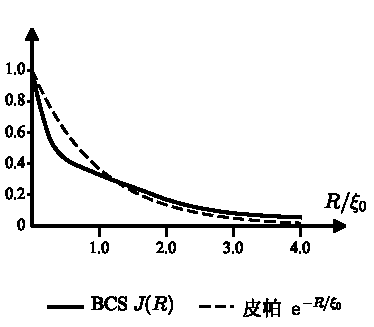
\includegraphics[width=6.5cm]{fig6-16.pdf}\\{\small 图 6.16}
\end{minipage}
\end{center}

\subsection*{5. 有限温度时的伦敦穿透深度}

在这里我们将用简单方法讨论 $T>0$ K时 $\lambda_{\mathrm{L}}(T)$ 随温度T的变化，具体计算超电流密度对弱磁场的线性响应
$\boldsymbol{j}(\boldsymbol{q},T)
=-\left(c/4\pi\right)K(q,T)\boldsymbol{A}(\boldsymbol{q})$，
并证明其系数K在伦敦极限 $\left(\boldsymbol{q}\to0\right)$ 满足
\begin{equation}
  K(q\to0,T)=\lambda_{\mathrm{L}}^{-2}(0)
  \left\{1-2\int_{\Delta}^{\infty}\mathrm{d}\xi\,
  \frac{\xi}{\sqrt{\xi^{2}-\Delta^{2}}}
  \left[-\frac{\partial f(\xi)}{\partial\xi}\right]\right\}
\end{equation}
其中 $\xi=\sqrt{\varepsilon^{2}+\Delta^{2}(T)}$，
$f(\xi)=\left[\exp\left(\beta\xi\right)+1\right]^{-1}$

首先讨论逆磁电流 $j_{2}$ 部分的贡献，根据式(6.8.11)，准至A一阶的有限温度 $j_{2}$ 在伦敦极限为
\begin{equation*}
\begin{aligned}
  \boldsymbol{j}_{2}(\boldsymbol{r},T)
  &=\langle\hat{\boldsymbol{j}}_{2}(\boldsymbol{r})\rangle_{T}\\
  &=-\frac{e^{2}}{mc}\boldsymbol{A}(\boldsymbol{r})
  \sum_{k,\,q}\mathrm{e}^{-\mathrm{i}\boldsymbol{q}\cdot\boldsymbol{r}}
  \left(\langle C^{+}_{k+q}C_{k}\rangle_{T}
  +\langle C^{+}_{-k}C_{-k-q}\rangle_{T}\right)\\
  &=-\frac{e^{2}}{mc}\boldsymbol{A}(\boldsymbol{r})
  \sum_{k}\left(\langle C^{+}_{k}C_{k}\rangle_{T}
  +\langle C^{+}_{-k}C_{-k}\rangle_{T}\right)\\
  &=-\frac{e^{2}}{mc}\boldsymbol{A}(\boldsymbol{r})\sum_{k}
  \left[1-\left(\varepsilon_{k}/\xi_{k}\right)
  \tanh\left(\frac{1}{2}\beta\xi_{k}\right)\right]
\end{aligned}
\end{equation*}
其中利用了平移对称性和习题(31)的结果.由于上式右边第二项是 $\varepsilon_{k}$ 的奇函数，它对于 $j_{2}$ 应无贡献，这时我们得到与零温情形式(6.8.12)相同的结果，再作傅里叶变换，可将其写为
\begin{equation*}
  \boldsymbol{j}_{2}(\boldsymbol{q},T)
  =-\frac{c}{4\pi}\lambda_{\mathrm{L}}^{-2}(0)\boldsymbol{A}(\boldsymbol{q})
  \equiv-\frac{c}{4\pi}K_{2}(q,T)\boldsymbol{A}(\boldsymbol{q})
\end{equation*}
表明逆磁电流的线性响应系数 $K_{2}$ 是一个与温度T和波数q均无关的量
\begin{equation}
  K_{2}(q,T)=\lambda_{\mathrm{L}}^{-2}(0)=\frac{4\pi ne^{2}}{mc^{2}}
\end{equation}
因此，总响应系数K的温度依赖只能来源于 $j_{1}$ 部分.类似于本节"1"中的讨论，取总哈密顿量
\begin{equation*}
  H=H_{0}+H_{1}
\end{equation*}
其中 $H_{0}$ 用无外磁场时系统的对角化哈密顿量式(6.4.23)表示
\begin{equation*}
  H_{0}=\sum_{k}\xi_{k}\left(\alpha^{+}_{k}\alpha_{k}
  +\alpha^{+}_{-k}\alpha_{-k}\right)+E_{\mathrm{s}}
\end{equation*}
而 $H_{1}$ 代表电子与外磁场的互作用，仍由式(6.8.8)表示.在伦敦极限 $\left(q\to0\right.$ 或 $\left.q\xi_{0}\ll1\right)$，由于式(6.8.8)等式右边第一项趋于零，而第二项的系数近似为1，这时 $H_{1}$ 可取为
\begin{equation}
  H_{1}\approx-\frac{e\hbar}{mc}\sum_{k}
  \left[\boldsymbol{k}\cdot\boldsymbol{A}(\boldsymbol{q})\right]
  \left(\alpha^{+}_{k}\alpha_{k}-\alpha^{+}_{-k}\alpha_{-k}\right)
\end{equation}
定义两种准粒子 $\alpha_{k}$ 与 $\alpha_{-k}$ 在弱外磁场中的重整化能量
\begin{equation}
  \left.
  \begin{aligned}
    \xi^{(-)}_{k}&\equiv\xi_{k}
    -\frac{e\hbar}{mc}\boldsymbol{k}\cdot\boldsymbol{A}(\boldsymbol{q})\\
    \xi^{(+)}_{k}&\equiv\xi_{k}
    +\frac{e\hbar}{mc}\boldsymbol{k}\cdot\boldsymbol{A}(\boldsymbol{q})
  \end{aligned}\right\}
\end{equation}
可将总哈密顿量H写成下列对角化的独立准粒子表示式：
\begin{equation}
  H=\sum_{k}\left(\xi^{(-)}_{k}\alpha^{+}_{k}\alpha_{k}
  +\xi^{(+)}_{k}\alpha^{+}_{-k}\alpha_{-k}\right)+E_{\mathrm{s}}
\end{equation}
再对式(6.8.13)取伦敦极限，得到
\begin{equation}
  \hat{\boldsymbol{j}}_{1}(\boldsymbol{r})\approx
  \left(\frac{e\hbar}{m}\right)\sum_{q}\mathrm{e}^{\mathrm{i}\boldsymbol{q}\cdot\boldsymbol{r}}
  \left\{\sum_{k}\boldsymbol{k}\left(\alpha^{+}_{k}\alpha_{k}
  -\alpha^{+}_{-k}\alpha_{-k}\right)\right\}
\end{equation}
其傅里叶分量
\begin{equation}
  \hat{\boldsymbol{j}}_{1}(\boldsymbol{q}\to0)\approx
  \left(\frac{e\hbar}{m}\right)\sum_{k}\boldsymbol{k}
  \left(\alpha^{+}_{k}\alpha_{k}-\alpha^{+}_{-k}\alpha_{-k}\right)
\end{equation}
与 $\boldsymbol{q}$ 无关，对上式求统计平均，并利用式(6.5.2)和式(6.8.43)可将 $j_{1}$ 的贡献表示为
\begin{equation}
\begin{aligned}
  \boldsymbol{j}_{1}(q\to0,T)&=\langle j_{1}(q\to0)\rangle\\
  &=\left(\frac{e\hbar}{m}\right)\sum_{k}\boldsymbol{k}
  \left(\langle\alpha^{+}_{k}\alpha_{k}\rangle_{T}
  -\langle\alpha^{+}_{-k}\alpha_{-k}\rangle_{T}\right)\\
  &=\left(\frac{e\hbar}{m}\right)\sum_{k}\boldsymbol{k}
  \left[f\left(\xi^{(-)}_{k}\right)-f\left(\xi^{(+)}_{k}\right)\right]
\end{aligned}
\end{equation}
由于在弱磁场时 $\xi^{(\pm)}_{k}$ 中含A项较小，可将 $f\left(\xi^{(\pm)}_{k}\right)$ 相对于 $f(\xi_{k})$ 作展开，求得
\begin{equation}
  f\left(\xi^{(-)}_{k}\right)-f\left(\xi^{(+)}_{k}\right)
  \approx-2\left[-\frac{\partial f}{\partial\xi_{k}}\right]
  \left(\frac{e\hbar}{mc}\right)
  \left[\boldsymbol{k}\cdot\boldsymbol{A}(\boldsymbol{q})\right]
\end{equation}
再代入式(6.8.46)，并将其中的缓变部分
$\boldsymbol{k}\left[\boldsymbol{k}\cdot\boldsymbol{A}(\boldsymbol{q})\right]$
用费密球面上的平均值 $\left[\dfrac{1}{3}k_{\mathrm{F}}^{2}
\boldsymbol{A}(\boldsymbol{q}\to0)\right]$ 代替，求得渐近式
\begin{equation}
\begin{aligned}
  \boldsymbol{j}_{1}(q\to0,T)
  &=\frac{2}{3}\left(\frac{e^{2}\hbar^{2}k_{\mathrm{F}}^{2}}{m^{2}c}\right)
  \boldsymbol{A}(q\to0)\sum_{k}
  \left[-\frac{\partial f(\xi_{k})}{\partial\xi_{k}}\right]\\
  &=\left\{\frac{4e^{2}E_{\mathrm{F}}}{3mc}\,g(0)\,2
  \int_{0}^{\infty}\mathrm{d}\varepsilon
  \left[-\frac{\partial f(\xi)}{\partial\xi}\right]\right\}
  \boldsymbol{A}(q\to0)\\
  &\equiv-\frac{c}{4\pi}K_{1}(q\to0,T)\boldsymbol{A}(q\to0)
\end{aligned}
\end{equation}
再考虑到费密面上正常金属的态密度 $g(0)=\left(3n/4E_{\mathrm{F}}\right)$ 和 $\xi\geqslant\Delta$ 时 $\left(\mathrm{d}\varepsilon/\mathrm{d}\xi\right)
=\xi/\sqrt{\xi^{2}-\Delta^{2}}$，可将 $j_{1}$ 的响应系数写为
\begin{equation}
  K_{1}(q\to0,T)=-\frac{2}{\lambda_{\mathrm{L}}^{2}(0)}
  \int_{\Delta}^{\infty}\mathrm{d}\xi\,
  \frac{\xi}{\sqrt{\xi^{2}-\Delta^{2}}}
  \left[-\frac{\partial f(\xi)}{\partial\xi}\right]
\end{equation}
因此，在弱外磁场中有限温度时总电流密度 $\boldsymbol{j}=\boldsymbol{j}_{1}+\boldsymbol{j}_{2}$ 的线性响应系数为
\begin{equation*}
\begin{aligned}
  K(q\to0,T)&=K_{1}(q\to0,T)+K_{2}(q\to0,T)\\
  &=\lambda_{\mathrm{L}}^{-2}(0)\left\{1-2\int_{\Delta}^{\infty}
  \mathrm{d}\xi\,\frac{\xi}{\sqrt{\xi^{2}-\Delta^{2}}}
  \left[-\frac{\partial f(\xi)}{\partial\xi}\right]\right\}\\
  &\equiv\lambda_{\mathrm{L}}^{-2}(T)
\end{aligned}
\end{equation*}
式(6.8.39)得证.

如果将 $\lambda_{\mathrm{L}}^{-2}(T)$ 写成与 $\lambda_{\mathrm{L}}^{-2}(0)$ 相似的形式
\begin{equation*}
  \lambda_{\mathrm{L}}^{-2}(T)\equiv 4\pi n_{\mathrm{s}}(T)\frac{e^{2}}{mc^{2}}
\end{equation*}
又可将 $T>0$ 的伦敦穿透深度表示为
\begin{equation}
\begin{aligned}
  \frac{n_{\mathrm{s}}(T)}{n}
  &\equiv\left[\frac{\lambda_{\mathrm{L}}(0)}{\lambda_{\mathrm{L}}(T)}\right]^{2}\\
  &=1-2\beta\int_{0}^{\infty}\frac{g_{\mathrm{s}}(\omega)}{g(0)}\,
  f(\omega)\left[1-f(\omega)\right]
\end{aligned}
\end{equation}
其中 $g_{\mathrm{s}}(\omega)$ 为超导体中准粒子的态密度，对于BCS超导体，根据式(6.6.19)
\begin{equation*}
  g_{\mathrm{s}}(\omega)=g(0)\,\mathrm{Re}\,
  \frac{|\omega|}{\sqrt{\omega^{2}-\Delta^{2}}}
\end{equation*}
作为一个练习［习题(34)］，读者不难导出伦敦穿透深度的渐近式
\begin{equation}
  \left[\frac{\lambda_{\mathrm{L}}(0)}{\lambda_{\mathrm{L}}(T)}\right]^{2}
  =\begin{cases}
    \displaystyle 2\left(1-\frac{T}{T_{\mathrm{c}}}\right)
    & \left(T_{\mathrm{c}}-T\ll T_{\mathrm{c}}\right)\\[1em]
    \displaystyle 1-\sqrt{\frac{2\pi\Delta(0)}{k_{\mathrm{B}}T}}\,
    \mathrm{e}^{-\Delta(0)/k_{\mathrm{B}}T}
    & \left(T\ll T_{\mathrm{c}}\right)
  \end{cases}
\end{equation}
特别是在低温区 $\left(T\ll T_{\mathrm{c}}\right)$，上式可简化为
\begin{equation}
  \frac{\Delta\lambda}{\lambda_{\mathrm{L}}(0)}
  =\frac{\lambda_{\mathrm{L}}(T)-\lambda_{\mathrm{L}}(0)}{\lambda_{\mathrm{L}}(0)}
  \approx\sqrt{\frac{\pi\Delta(0)}{2k_{\mathrm{B}}T}}\,
  \mathrm{e}^{-\Delta(0)/k_{\mathrm{B}}T}
  \qquad(T\ll T_{\mathrm{c}})
\end{equation}
表现出在低温时 $\Delta\lambda(T)\sim\mathrm{e}^{-\beta\Delta(0)}$ 的指数激发特征，与低温比热容 $c_{\mathrm{es}}\sim\mathrm{e}^{-\beta\Delta(0)}$ 的特征相似.此外，式(6.8.50)也适用于各向异性超导体，我们将在第七章中作专门的介绍.式(6.8.50)也可以看作是有限温度超导电子浓度 $n_{\mathrm{s}}(T)$ 的定义式.当 $T=0$ K时，由于没有准粒子激发，等式右边第二项为零，得到 $n_{\mathrm{s}}(0)=n$.但是，当 $T>0$ K时，由于实际上还存在着准粒子激发 $\left(n_{\mathrm{QP}}\neq0\right)$，应有关系式 $n_{\mathrm{s}}(T)=n-n_{\mathrm{QP}}(T)$，这时式(6.8.50)等式右边第二项实际上代表比值 $n_{\mathrm{QP}}(T)/n$.因此，在 $0<T<T_{\mathrm{c}}$ 温区内，随着T升高QP的激发 $\left(n_{\mathrm{QP}}/n\right)$ 增大，相应的超导电子浓度 $n_{\mathrm{s}}(T)$ 减小，使得屏蔽磁场的超电流减弱，这就是 $\lambda_{\mathrm{L}}(T)$ 随温度上升而增大的物理原因.

\section{BCS超导体中的粒子数和相位}

以上讨论限于 $\Delta$ 为实量.在一般情况下，对势 $\Delta$ 是一个复量，我们应当设
\begin{equation}
  \left.
  \begin{aligned}
    \Delta&=V\sum_{k}\langle C_{-k}C_{k}\rangle=|\Delta|\,\mathrm{e}^{\mathrm{i}\varphi}\\
    \Delta^{*}&=V\sum_{k}\langle C^{+}_{k}C^{+}_{-k}\rangle
    =|\Delta|\,\mathrm{e}^{-\mathrm{i}\varphi}
  \end{aligned}\right\}
\end{equation}
所对应的自洽场近似（SCFA）的哈密顿量与式(6.4.6)略有不同
\begin{equation}
  \overline{H}=\sum_{k}\varepsilon_{k}
  \left(C^{+}_{k}C_{k}+C^{+}_{-k}C_{-k}\right)
  -\sum_{k}\left(\Delta C^{+}_{k}C^{+}_{-k}
  +\Delta^{*}C_{-k}C_{k}\right)+|\Delta|^{2}/V
\end{equation}
对角化的 $u$-$v$ 变换仍与式(6.4.9)相似
\begin{equation}
  \left.
  \begin{aligned}
    \alpha_{k}&=u_{k}C_{k}-v_{k}C^{+}_{-k}\\
    \alpha_{-k}&=u_{k}C_{-k}+v_{k}C^{+}_{k}
  \end{aligned}\right\}
\end{equation}
但 $u_{k}$ 与 $v_{k}$ 也应取为复量.其逆变换与式(6.4.15)则不相同
\begin{equation}
  \left.
  \begin{aligned}
    C_{k}&=u^{*}_{k}\alpha_{k}+v_{k}\alpha^{+}_{-k}\\
    C_{-k}&=u^{*}_{k}\alpha_{-k}-v_{k}\alpha^{+}_{k}
  \end{aligned}\right\}
\end{equation}
而与式(6.4.17)相应的对角化条件变为
\begin{equation}
  \Delta u_{k}^{2}-\Delta^{*}v_{k}^{2}=2\varepsilon_{k}u_{k}v_{k}
\end{equation}
其中
\begin{equation}
  |u_{k}|^{2}+|v_{k}|^{2}=1
\end{equation}
用 $\left(\Delta^{*}/u_{k}^{2}\right)$ 乘式(6.9.5)的等式两边，得到
\begin{equation}
  \left(\Delta^{*}\frac{v_{k}}{u_{k}}\right)^{2}
  +2\varepsilon_{k}\left(\Delta^{*}\frac{v_{k}}{u_{k}}\right)
  -|\Delta|^{2}=0
\end{equation}
其稳定解为
\begin{equation}
  \Delta^{*}\left(\frac{v_{k}}{u_{k}}\right)=\xi_{k}-\varepsilon_{k}
\end{equation}
其中 $\xi_{k}=\sqrt{\varepsilon_{k}^{2}+|\Delta|^{2}}$ 代表元激发能量，与取 $\Delta$ 为实量时的结果完全一样，只要记住在式(6.4.19)中 $\Delta^{2}\equiv|\Delta|^{2}=\Delta^{*}\Delta$.再利用式(6.9.6)即可求出
\begin{equation}
  \left.
  \begin{aligned}
    |u_{k}|^{2}&=\frac{1}{2}\left(1+\varepsilon_{k}/\xi_{k}\right)\\
    |v_{k}|^{2}&=\frac{1}{2}\left(1-\varepsilon_{k}/\xi_{k}\right)
  \end{aligned}\right\}
\end{equation}
也与 $u_{k}$ 和 $v_{k}$ 均为实量时的结果完全一致.注意到式(6.9.8)等式右边的量 $\left(\xi_{k}-\varepsilon_{k}\right)$ 为实量，按此 $\Delta^{*}\left(\dfrac{v_{k}}{u_{k}}\right)$ 也应是实数，于是得到
\begin{equation}
  \frac{v_{k}}{u_{k}}
  =\Delta\left[\frac{\left(\xi_{k}-\varepsilon_{k}\right)}{|\Delta|^{2}}\right]
\end{equation}
上式表明 $v_{k}$ 相对于 $u_{k}$ 的相位与能隙 $\Delta$ 的相位相同，这是一个重要的结果.

BCS超导体的基态波函数仍可写成式(6.4.38)的形式，只是现在 $u_{k}$ 与 $v_{k}$ 应为复量.由于在量子力学中允许总波函数相差一个相位因子，我们可以进一步设 $u_{k}$ 为实，而仅取 $v_{k}$ 为复量
\begin{equation}
  u_{k}=|u_{k}|\text{，}
  \qquad v_{k}=|v_{k}|\,\mathrm{e}^{\mathrm{i}\varphi_{k}}
\end{equation}
这时 $\varphi_{k}$ 正好代表 $v_{k}$ 相对于 $u_{k}$ 的相位差，再根据式(6.9.10)和式(6.9.1)可以求出
\begin{equation}
  \varphi_{k}=\varphi
\end{equation}
这是一个非常重要的结果，它表明：在BCS超导体中在任一 $(\boldsymbol{k}\uparrow,-\boldsymbol{k}\downarrow)$ 态上被一对电子占据时的概率幅 $v_{k}$ 的相位差是与k无关的一个常数.换句话说，所有在费密面附近凝聚的电子对都具有相同的相位差 $\varphi$.在这个意义上，人们常说BCS的超导基态是一种相位相干态.这时基态波函数应写为
\begin{equation}
  |\varphi\rangle=\prod_{k}
  \left(|u_{k}|+|v_{k}|\,\mathrm{e}^{\mathrm{i}\varphi}
  C^{+}_{k}C^{+}_{-k}\right)|\mathrm{VAC}\rangle
\end{equation}
其中 $\varphi$ 可取0到 $2\pi$ 之间的任一确定值.显然，前面的式(6.4.38)代表 $\varphi=0$ 的特殊相位情形，并且 $u_{k}=|u_{k}|$，$v_{k}=|v_{k}|$.在一般情况下，最好保留 $\varphi$ 而写成在(6.9.13)的形式，因为由此可导出粒子数与相位之间的不确定关系.

仔细考察式(6.9.13)，不难发现在 $|\varphi\rangle$ 中粒子数N严格确定的状态 $|N\rangle$ 是其乘积展开式中含有 $\dfrac{N}{2}$ 个 $\mathrm{e}^{\mathrm{i}\varphi}$ 因子的项，根据安德逊的做法，可以通过下面的相位积分取出 $|\varphi\rangle$ 中含N个粒子状态的分量
\begin{equation}
  |N\rangle=\frac{1}{2\pi}\int_{0}^{2\pi}\mathrm{d}\varphi\,
  \mathrm{e}^{-\mathrm{i}N\varphi/2}|\varphi\rangle
\end{equation}
上式中对相位 $\varphi$ 的所有可能取值作积分，也就是使相位 $\varphi$ 完全不确定，这时我们才可以得到完全确定粒子数N的状态，而其逆变换为
\begin{equation}
  |\varphi\rangle=\sum_{N=0}^{\infty}\mathrm{e}^{\mathrm{i}N\varphi/2}|N\rangle
\end{equation}
从物理上讲，确定的相位 $\varphi$，对应于总粒子数不守恒的情况，这是BCS基态波函数的一个重要特征.显然，$|N\rangle$ 和 $|\varphi\rangle$ 之间的变换关系与量子力学中共轭量 $\boldsymbol{p}$ 和x之间的本征函数 $|\boldsymbol{p}\rangle$ 和 $|\boldsymbol{x}\rangle$ 的变换关系相似.可以认为N与 $\varphi$ 也是一对共轭力学量，并且可将 $\dfrac{N}{2}$ 对应于 $\boldsymbol{p}$，$\hbar\varphi$ 对应于x，再根据不确定关系式
$\Delta p\,\Delta x\geqslant\dfrac{\hbar}{2}$，求出N与 $\varphi$ 间相应的不确定关系
\begin{equation}
  \Delta N\,\Delta\varphi\gtrsim1
\end{equation}
它同样地反映了系统的量子特性，表明同时测量N和 $\varphi$ 的精度有一个限制.

现在我们转入对BCS超导体中确定粒子数和相位的精度作定性的讨论.在BCS超导基态中的平均粒子数 $\overline{N}$ 由粒子数算符
$\hat{N}=\sum_{k}\left(C^{+}_{k}C_{k}+C^{+}_{-k}C_{-k}\right)$
的基态平均决定，当取 $\varphi=0$ 时，习题(30)中已证明
\begin{equation}
  \overline{N}=\langle0|\hat{N}|0\rangle
  =2\sum_{k}v_{k}^{2}
  =\frac{\Omega}{(2\pi)^{3}}\int\mathrm{d}^{3}k\,\left(2v_{k}^{2}\right)
\end{equation}
而其均方涨落也已求出为
\begin{equation}
  \langle\hat{N}^{2}\rangle-\langle\hat{N}\rangle^{2}
  =\sum_{k}4u_{k}^{2}v_{k}^{2}
  =\frac{\Omega}{(2\pi)^{3}}\int\mathrm{d}^{3}k\,
  \left(4u_{k}^{2}v_{k}^{2}\right)
\end{equation}
在这里 $\Omega$ 代表样品的体积.在热力学极限（当 $\overline{N}\to\infty$ 和 $\Omega\to\infty$，但两者比值固定时），可根据均方涨落正比于体积 $\Omega$，断定它必然正比于 $\overline{N}$.按此求出均方根涨落，即 $\Delta N$ 为
\begin{equation}
  \Delta N=\sqrt{\langle(\hat{N}-\overline{N})^{2}\rangle}
  =\sqrt{\langle\hat{N}^{2}\rangle-\overline{N}^{2}}
  \approx\overline{N}^{1/2}
\end{equation}
由于 $\overline{N}\sim10^{20}$，可取 $\Delta N\sim10^{10}$，代入不确定关系式(6.9.16)，求得 $\varphi=0$ 时的位相涨落 $\Delta\varphi\sim10^{-10}$ 是一个很小的量，说明BCS超导体中相位涨落很小.另一方面，尽管均方根涨落 $\Delta N$ 较大，但在BCS基态中粒子数的相对涨落
$\left(\dfrac{\Delta N}{\overline{N}}\right)\sim\dfrac{1}{\overline{N}^{1/2}}
\sim10^{-10}$ 却是很小的.换句话说，在BCS基态中 $\left(\Delta N/\overline{N}\right)$ 和 $\Delta\varphi$ 都近似在 $\overline{N}^{-1/2}\sim10^{-10}$ 的数量级范围内可被确定.

以上讨论表明：BCS超导体中相位 $\varphi$ 与粒子数N是一对共轭力学量，满足不确定关系式(6.9.16).另一方面，允许 $\varphi$ 取特定值（包括在本章§4中取 $\varphi=0$ 情形）则对应于BCS超导体中的相位相干和总粒子数不守恒等两项重要特性.在空间非均匀情况下，当涉及两块超导体的连接系统时，对势 $\Delta$ 中所含相位因子 $\mathrm{e}^{\mathrm{i}\varphi}$ 将起重要的作用，涉及库柏对在两块弱连接超导体间的隧穿问题.我们将在下一节中采用唯象的金兹堡-朗道理论对超导体中的相位相干特征作进一步的探讨，涉及超导体中的约瑟夫森效应.

\section{金兹堡-朗道方程}

在伦敦方程中，超导电子密度与磁场及空间位置无关，因此它只适用于讨论弱磁场中的均匀超导体问题，而不能处理非均匀超导体（如超导体与正常体的S-N界面等问题）和强磁场情况.为计及超导电子密度随空间位置的变化，金兹堡和朗道\textsuperscript{[9]}（后简称G-L）建议用一个复量 $\psi(\boldsymbol{r})$ 作为超导电子的"有效波函数"，$\psi(\boldsymbol{r})$ 与超导电子的局域密度 $n_{\mathrm{s}}(\boldsymbol{r})$ 有如下关系：
\begin{equation}
  |\psi(\boldsymbol{r})|^{2}=n_{\mathrm{s}}(\boldsymbol{r})
\end{equation}
对于正常态 $n_{\mathrm{s}}=0$，$\psi=0$，而超导态 $n_{\mathrm{s}}\neq0$，$\psi\neq0$.因此 $\psi$ 起序参数作用，这是一个复序参数.由于超导-正常转变是二级相变，$T\to T_{\mathrm{c}}$ 时 $n_{\mathrm{s}}\to0$，在转变点附近 $\psi$ 应为小量，可以将自由能展开为序参量 $|\psi|^{2}$ 的幂级数，并计及磁场 $\boldsymbol{B}=\nabla\times\boldsymbol{A}$ 的影响，利用自由能泛函的极小确定空间各点的序参数方程和电流密度方程（G-L方程），这就是金兹堡-朗道唯象理论的基本精神.理论主要用于 $T_{\mathrm{c}}-T\ll T_{\mathrm{c}}$ 温区.

\subsection*{1. G-L自由能}

对于均匀超导体，当外场为零时在 $T_{\mathrm{c}}$ 附近自由能密度 $f_{\mathrm{s}}$ 可按小量 $n_{\mathrm{s}}$ 展开
\begin{equation*}
  f_{\mathrm{s}}=f_{\mathrm{n}}+\alpha(T)n_{\mathrm{s}}
  +\frac{1}{2}\beta(T)n_{\mathrm{s}}^{2}+\cdots
\end{equation*}
略去高阶项，并利用式(6.10.1)将上式改写成序参量的展式
\begin{equation}
  f_{\mathrm{s}}=f_{\mathrm{n}}+\alpha(T)|\psi(\boldsymbol{r})|^{2}
  +\frac{1}{2}\beta(T)|\psi(\boldsymbol{r})|^{4}
\end{equation}
其中 $f_{\mathrm{n}}$ 为零磁场时正常态的自由能密度.$\alpha$、$\beta$ 是与温度有关的唯象参数，可利用自由能极小定出
\begin{equation}
  n_{\mathrm{s}}=|\psi(\boldsymbol{r})|^{2}
  =-\frac{\alpha(T)}{\beta(T)}
\end{equation}
由于 $T<T_{\mathrm{c}}$ 时 $n_{\mathrm{s}}>0$，因此式(6.10.3)要求 $\left(\alpha/\beta\right)<0$，将式(6.10.3)代入式(6.10.2)，得
\begin{equation}
  f_{\mathrm{n}}-f_{\mathrm{s}}=\frac{1}{2}\frac{\alpha^{2}(T)}{\beta(T)}
  =\frac{1}{8\pi}H_{\mathrm{c}}^{2}(T)
\end{equation}
最后一个等式中的 $H_{\mathrm{c}}(T)$ 是破坏超导的临界磁场，这里利用了熟知的超导热力学关系，式(6.10.4)要求 $\beta(T)>0$.又因为 $T=T_{\mathrm{c}}$ 时 $n_{\mathrm{s}}=0$，从公式(6.10.3)还可得知 $\alpha(T_{\mathrm{c}})=0$ 和 $\beta(T_{\mathrm{c}})\neq0$，因此在 $T_{\mathrm{c}}-T\ll T_{\mathrm{c}}$ 温区，$\alpha$、$\beta$ 可表示成
\begin{equation}
  \left.
  \begin{aligned}
    \alpha(T)&=\left(T-T_{\mathrm{c}}\right)
    \left(\frac{\mathrm{d}\alpha}{\mathrm{d}T}\right)_{T_{\mathrm{c}}}\\
    \beta(T)&\approx\beta\left(T_{\mathrm{c}}\right)
  \end{aligned}\right\}
\end{equation}
由式(6.10.4)与式(6.10.5)，得 $f_{\mathrm{n}}-f_{\mathrm{s}}\sim\left(T_{\mathrm{c}}-T\right)^{2}$.因此，$H_{\mathrm{c}}\sim\left(T_{\mathrm{c}}-T\right)$，与实验相符，并反映了转变点附近二级相变的共同特征.

式(6.10.2)只是均匀超导体的朗道二级相变公式.假如 $\psi$ 随位置 $\boldsymbol{r}$ 变化，还需在式(6.10.2)中计入 $\psi$ 的导数项对 $f_{\mathrm{s}}$ 的影响.当 $|\psi|^{2}$ 变化缓慢时，G-L取磁场矢量 $\boldsymbol{A}=0$ 时的附加能量为
\begin{equation*}
  \frac{1}{2m^{*}}\left|-\mathrm{i}\hbar\nabla\psi(\boldsymbol{r})\right|^{2}
\end{equation*}
与有效质量为 $m^{*}$，波函数为 $\psi$ 的"粒子"的动能项相似.物理上可理解为 $\boldsymbol{A}=0$ 时，$\nabla\psi\neq0$，对应于超导体的载流状态，因此有上述类似动能项出现.

推广到 $\boldsymbol{A}(\boldsymbol{r})\neq0$ 情况，可根据电动力学将 $-\mathrm{i}\hbar\nabla$ 换成为正则动量 $-\mathrm{i}\hbar\nabla-\dfrac{e^{*}}{c}\boldsymbol{A}$，则自由能密度的附加项为
\begin{equation*}
  \frac{1}{2m^{*}}\left|\left(-\mathrm{i}\hbar\nabla
  -\frac{e^{*}}{c}\boldsymbol{A}\right)\psi(\boldsymbol{r})\right|^{2}
\end{equation*}
好像电荷为 $e^{*}$、质量为 $m^{*}$ 的粒子在磁场中运动的动能项.这是G-L理论中的主要假定.再计及磁场能量 $\dfrac{1}{8\pi}|\nabla\times\boldsymbol{A}|^{2}$，即得G-L的自由能展开式
\begin{equation}
\begin{aligned}
  f_{\mathrm{s}}&=f_{\mathrm{n}}+\alpha(T)|\psi(\boldsymbol{r})|^{2}
  +\frac{1}{2}\beta(T)|\psi(\boldsymbol{r})|^{4}\\
  &\quad+\frac{1}{8\pi}\left(\nabla\times\boldsymbol{A}\right)
  \cdot\left(\nabla\times\boldsymbol{A}\right)
  +\frac{1}{2m^{*}}\left|\left(-\mathrm{i}\hbar\nabla
  -\frac{e^{*}}{c}\boldsymbol{A}\right)\psi(\boldsymbol{r})\right|^{2}
\end{aligned}
\end{equation}
系统的自由能为
\begin{equation}
  F_{\mathrm{s}}=\int f_{\mathrm{s}}\,\mathrm{d}\boldsymbol{r}
\end{equation}

\subsection*{2. G-L方程}

利用热力学平衡条件，要求自由能对序参数和磁场矢量势的任意变化 $\delta\psi$、$\delta\psi^{*}$ 及 $\delta\boldsymbol{A}$ 为极小，可求出G-L方程.根据式(6.10.6)与(6.10.7)，求得自由能的变分为
\begin{equation}
\begin{aligned}
  \delta F_{\mathrm{s}}&=\delta\int f_{\mathrm{s}}\,\mathrm{d}\boldsymbol{r}\\
  &=\int\mathrm{d}\boldsymbol{r}\biggl\{\delta\psi^{*}
  \left[\alpha\psi+\beta|\psi|^{2}\psi
  +\frac{1}{2m^{*}}\left(-\mathrm{i}\hbar\nabla
  -\frac{e^{*}}{c}\boldsymbol{A}\right)^{2}\psi\right]
  +\mathrm{c.c.}\biggr\}+\\
  &\quad\int\mathrm{d}\boldsymbol{r}\biggl\{\delta\boldsymbol{A}\cdot
  \left[\frac{\nabla\times\nabla\times\boldsymbol{A}}{4\pi}
  +\frac{\mathrm{i}\hbar e^{*}}{2m^{*}c}
  \left(\psi^{*}\nabla\psi-\psi\nabla\psi^{*}\right)\right.\\
  &\quad\left.+\left(\frac{e^{*}}{c}\right)^{2}
  \frac{1}{m^{*}}\boldsymbol{A}\,|\psi|^{2}\right]+\mathrm{c.c.}\biggr\}
\end{aligned}
\end{equation}
其中 $\mathrm{c.c.}$ 代表复共轭项.在推导式(6.10.8)过程中还假设了下列面积分为零
\begin{equation*}
  \int_{\mathrm{s}}\mathrm{d}S\left\{\delta\psi^{*}
  \left(-\mathrm{i}\hbar\nabla-\frac{e^{*}}{c}\boldsymbol{A}\right)_{n}\psi
  +\mathrm{c.c.}\right\}=0
\end{equation*}
下标n表示垂直表面方向的分量，相当于一个边界条件
\begin{equation}
  \left(-\mathrm{i}\hbar\nabla-\frac{e^{*}}{c}\boldsymbol{A}\right)_{n}
  \psi(\boldsymbol{r})=0
\end{equation}
要求 $\delta F_{\mathrm{s}}=0$，由式(6.10.8)可得下列方程：
\begin{equation}
  \frac{1}{2m^{*}}\left(-\mathrm{i}\hbar\nabla
  -\frac{e^{*}}{c}\boldsymbol{A}\right)^{2}\psi
  +\alpha\psi+\beta|\psi|^{2}\psi=0
\end{equation}
\begin{equation}
  \boldsymbol{j}=\frac{c}{4\pi}\nabla\times\boldsymbol{B}
  =-\frac{\mathrm{i}\hbar e^{*}}{2m^{*}}
  \left(\psi^{*}\nabla\psi-\psi\nabla\psi^{*}\right)
  -\frac{\left(e^{*}\right)^{2}}{m^{*}c}|\psi|^{2}\boldsymbol{A}
\end{equation}
这就是著名的金斯堡-朗道（G-L）方程.式(6.10.10)类似粒子在磁场中运动的薛定谔方程，但应注意它是非线性的，是确定序参数 $\psi$ 的方程.式(6.10.11)就是量子力学的电流密度公式.

\subsection*{3. G-L参数 $\kappa$}

G-L方程是非线性的联立方程，其一般解相当复杂，这里仅介绍一些简单解，主要目的是引入特征参量 $\xi(T)$、$\lambda(T)$ 和 $\kappa(T)$.

（i）序参数的空间变化范围 $\xi(T)$

G-L方程有如下两个最简单的解.

（1）$\psi=0$，而A仅仅由 $\boldsymbol{B}=\nabla\times\boldsymbol{A}$ 决定，$\boldsymbol{B}=\boldsymbol{H}$ 为外场，这个解描述正常态.

（2）$\psi=\psi_{0}=\left[-\alpha(T)/\beta(T)\right]^{\frac{1}{2}}$ 和 $\boldsymbol{A}=0$.这个解代表具有完全迈斯纳效应（忽略表面效应）的超导状态.$\psi_{0}$ 是与 $\boldsymbol{r}$ 无关的空间均匀解，这时系统具有最低自由能 $\left(T<T_{\mathrm{c}}\right.$，$\left.\alpha<0\right.$ 时$)$，如式(6.10.4).因此，人们常常说无外场时大块超导体的平衡态为序参数 $\psi=\psi_{0}=$ 常数\footnote{确切地说，$\psi_{0}$ 只是大块超导样品远离界面处的序参数值.}.

现在讨论磁场非常弱的情况，根据(2)不难预料 $\psi$ 的空间变化将十分缓慢.$\psi$ 与 $\psi_{0}$ 很接近，在G-L的第一个方程(6.10.10)中可令 $\boldsymbol{A}=0$，再引入量纲为1的序参数
\begin{subequations}
\begin{equation}
  f\equiv\frac{\psi}{\psi_{0}}\text{，}
  \qquad \psi_{0}=\sqrt{\frac{|\alpha|}{\beta}}
\end{equation}
其中f满足方程
\begin{equation}
  -\frac{\hbar^{2}}{2m^{*}\alpha}\nabla^{2}f+f-f^{3}=0
\end{equation}
\end{subequations}
由上式可定义一个特征长度 $\xi(T)$
\begin{equation}
  \xi^{2}(T)\equiv-\frac{\hbar^{2}}{2m^{*}\alpha(T)}
\end{equation}
它代表序参数（f及 $\psi$）的空间变化尺度.为了更清楚地说明 $\xi(T)$ 的性质，我们考虑以 $z=0$ 为界的N-S问题 $\left(z<0\right.$ 为正常体N，$z>0$ 为超导体S$)$.这时式(6.10.12b)简化为
\begin{equation}
  \xi^{2}\frac{\mathrm{d}^{2}f}{\mathrm{d}z^{2}}=-f\left(1-f^{2}\right)
  \qquad(z\geqslant0)
\end{equation}
边界条件为 $z=0$ 时，序参数 $f=0$.上式乘 $\left(\mathrm{d}f/\mathrm{d}z\right)$ 后积分，得出
\begin{equation}
  \xi^{2}\left(\frac{\mathrm{d}f}{\mathrm{d}z}\right)^{2}
  =\frac{1}{2}\left(1-f^{2}\right)^{2}
\end{equation}
这里积分常数由 $f^{2}\to1$ 时 $\mathrm{d}f/\mathrm{d}z\to0$ 决定.由于z增大时f增大，上式取正根
$\dfrac{\mathrm{d}f}{\mathrm{d}z}=\dfrac{1-f^{2}}{\sqrt{2}\,\xi(T)}$，求得
\begin{equation}
  f(z)=\tanh\frac{z}{\sqrt{2}\,\xi(T)}
  \qquad(z\geqslant0)
\end{equation}
由此可见，$f(z)$ 的空间变化范围是 $\xi(T)$，这个量称为G-L相干长度，它和温度的关系为
\begin{equation}
  \xi(T)=\frac{\hbar}{\left[2m^{*}\left(T_{\mathrm{c}}-T\right)
  \alpha'\left(T_{\mathrm{c}}\right)\right]^{1/2}}
\end{equation}
其中 $\alpha'\left(T_{\mathrm{c}}\right)=\left(\dfrac{\mathrm{d}\alpha}{\mathrm{d}T}\right)_{T_{\mathrm{c}}}$.当 $T\to T_{\mathrm{c}}$ 时，$\xi(T)\to\infty$.注意，$\xi(T)$ 与BCS相干长度 $\xi_{0}=\dfrac{\hbar v_{\mathrm{F}}}{\pi\Delta(0)}$ 不是同一个量.图6.17中实线表示在N-S界面序参数的变化曲线，而虚线代表磁场的穿透情况.

（ii）弱场穿透深度 $\lambda(T)$

G-L第二方程(6.10.11)在准至磁场一阶时可用无磁场时的 $\psi_{0}^{2}$ 代替其中的 $|\psi|^{2}$，从而求得电流密度j为
\begin{equation}
  \boldsymbol{j}=-\frac{\mathrm{i}\hbar e^{*}}{2m^{*}}
  \left(\psi^{*}\nabla\psi-\psi\nabla\psi^{*}\right)
  -\frac{\left(e^{*}\right)^{2}}{m^{*}c}\psi_{0}^{2}\boldsymbol{A}
\end{equation}
若令 $\psi=\psi_{0}+\psi_{1}$，$\psi_{1}$ 为含A一阶的序参量，由于 $\psi_{0}$ 与 $\boldsymbol{r}$ 无关，上式右边第一项最低阶是 $\boldsymbol{A}^{2}$ 项.因此，准至A一阶的电流公式为
\begin{equation}
\begin{aligned}
  \boldsymbol{j}(\boldsymbol{r})
  &=-\frac{\left(e^{*}\right)^{2}}{m^{*}c}\psi_{0}^{2}\boldsymbol{A}(\boldsymbol{r})\\
  &=-\frac{c}{4\pi}\left[\frac{4\pi\left(e^{*}\right)^{2}\psi_{0}^{2}}
  {m^{*}c^{2}}\right]\boldsymbol{A}(\boldsymbol{r})
\end{aligned}
\end{equation}
与伦敦方程式(6.7.8)相比较，求得穿透深度
\begin{equation}
  \lambda(T)=\left[\frac{m^{*}c^{2}}
  {4\pi\left(e^{*}\right)^{2}\psi_{0}^{2}}\right]^{1/2}
\end{equation}
再利用式(6.10.12a)和式(6.10.5)，可将 $\lambda(T)$ 表示为
\begin{equation}
  \lambda(T)=\left[\frac{m^{*}c^{2}\beta\left(T_{\mathrm{c}}\right)}
  {4\pi\left(e^{*}\right)^{2}\left(T_{\mathrm{c}}-T\right)
  \alpha'\left(T_{\mathrm{c}}\right)}\right]^{1/2}
\end{equation}
显然，在 $T_{\mathrm{c}}-T\ll T_{\mathrm{c}}$ 温区内，$\lambda(T)$ 与G-L相干长度的表示式(6.10.17)相似，它们都与 $\left(T_{\mathrm{c}}-T\right)^{-1/2}$ 成正比，并且 $\lambda(T)$ 与 $\xi(T)$ 的比值是一个与温度无关的特性常数 $\kappa$
\begin{equation}
  \kappa\equiv\frac{\lambda(T)}{\xi(T)}
  =\frac{m^{*}c}{\hbar e^{*}}\left(\frac{\beta}{2\pi}\right)^{1/2}
\end{equation}
称为G-L参数.利用 $\psi_{0}^{2}=\dfrac{|\alpha|}{\beta}$ 和式(6.10.4)，有
$|\alpha|\psi_{0}^{2}=\dfrac{1}{4\pi}H_{\mathrm{c}}^{2}(T)$，
再利用式(6.10.13)与式(6.10.20)，我们还可以将 $\kappa$ 表示为
\begin{equation}
  \kappa=\frac{\sqrt{2}\,e^{*}}{\hbar c}H_{\mathrm{c}}(T)\lambda^{2}(T)
\end{equation}
说明G-L参数 $\kappa$ 可由测量直接决定.再考虑到 $\kappa=\lambda(T)/\xi(T)$，我们又可求得诸特征量 $H_{\mathrm{c}}(T)$、$\lambda(T)$ 和 $\xi(T)$ 之间的一个重要关系式
\begin{equation}
  H_{\mathrm{c}}(T)\lambda(T)\xi(T)
  =\frac{1}{2\pi\sqrt{2}}\left(\frac{2\pi\hbar c}{e^{*}}\right)
\end{equation}
即三者的乘积为一常数，其中 $\left(2\pi\hbar c/e^{*}\right)$ 正是下面将要介绍的超导磁通量子.

G-L参数 $\kappa$ 是超导体分类的重要参数.根据图6.17在正常与超导物质之间存在着由N到S的过渡层.在过渡层中磁场连续下降为零.序参数 $\psi$ 则由零连续上升到S区深部的数值 $\psi_{0}$，这就是N-S界面区.由于磁场透入界面区和序参数在界面区下降所引起单位面积吉布斯自由能的变化称为界面能.界面能与 $\xi(T)$ 和 $\lambda(T)$ 的相对大小有关，与超导体的特征密切相关.

\begin{center}
\begin{minipage}{8cm}
\centering
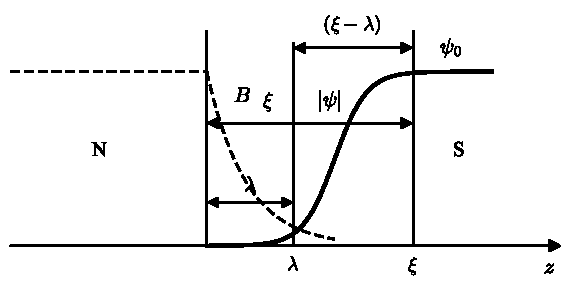
\includegraphics[width=8cm]{fig6-17.pdf}\\{\small 图 6.17\quad N-S界面区的有序参数变化}
\end{minipage}
\end{center}

为估计界面能的大小，可以将图6.17近似看作磁场 $H_{\mathrm{c}}$ 完全透入到 $0<z<\lambda(T)$ 区域，而在 $z\geqslant\lambda(T)$ 区近似为零.有序参数 $\psi$ 的变化也可当作在 $0<z<\xi(T)$ 范围内近似取零值，而在 $z\geqslant\xi(T)$ 区取 $\psi_{0}$ 值.这样，在 $\lambda<z<\xi$ 区域内序参数 $\psi$ 和B均为零，相当于无外场时的正常态，其吉布斯自由能密度显然应比纯超导态高 $H_{\mathrm{c}}^{2}/8\pi$.由于这个区域的存在所引起单位面积自由能的改变为
\begin{equation*}
  \left(\xi-\lambda\right)\frac{H_{\mathrm{c}}^{2}}{8\pi}
\end{equation*}
在 $0<z<\lambda(T)$ 区内，虽然也从原来的超导态变成了正常态，自由能密度将增加 $H_{\mathrm{c}}^{2}/8\pi$，但是由于磁场 $H_{\mathrm{c}}$ 的完全透入，吉布斯自由能密度将减少同一数值，因此 $0<z<\lambda(T)$ 区域相对于原来的纯超导态能量没有变化.于是，N-S的界面能大致为
\begin{equation}
  \sigma_{\mathrm{ns}}\approx\left(\xi-\lambda\right)\frac{H_{\mathrm{c}}^{2}}{8\pi}
\end{equation}
当 $\xi>\lambda$ 时 $\sigma_{\mathrm{ns}}>0$，界面能为正，而当 $\xi<\lambda$ 时 $\sigma_{\mathrm{ns}}<0$，界面能为负，分别属于两种不同类型的超导体.若用G-L方程严格计算界面能\textsuperscript{[10]}，可求得比式(6.10.25)更精确的结果；当 $\kappa=1/\sqrt{2}$ 时 $\sigma_{\mathrm{ns}}=0$，而
\begin{equation*}
  \kappa<\frac{1}{\sqrt{2}}\text{，}\qquad \sigma_{\mathrm{ns}}>0
  \qquad\text{（Ⅰ类超导体）}
\end{equation*}
\begin{equation*}
  \kappa>\frac{1}{\sqrt{2}}\text{，}\qquad \sigma_{\mathrm{ns}}<0
  \qquad\text{（Ⅱ类超导体）}
\end{equation*}
$\kappa<1/\sqrt{2}$ 的超导材料，具有正界面能，磁场若透入超导体必将在样品内部产生正常区，从而形成N-S界面，但由于 $\sigma_{\mathrm{ns}}>0$ 在能量上是不利的，因此Ⅰ类超导体在 $H<H_{\mathrm{c}}$ 时序参数保持均匀分布，磁场不能透入内部，样品具有完全逆磁性.当 $\kappa>1/\sqrt{2}$ 时，情况相反，在一定条件下，磁场能透入样品内部，形成许多正常区，因为这时 $\sigma_{\mathrm{ns}}<0$，界面增加在能量上是有利的.这类材料称为Ⅱ类超导体，它不具有完全逆磁性.

\subsection*{4. 磁通量子化}

从G-L的超导电流方程(6.10.11)可以证实伦敦的磁通量子化假定.将复序参数写成
\begin{equation*}
  \psi=|\psi|\,\mathrm{e}^{\mathrm{i}\varphi}
\end{equation*}
形式，$\varphi$ 为实量，代入式(6.10.11)求得
\begin{equation}
  \boldsymbol{j}=\frac{e^{*}\hbar}{m^{*}}|\psi|^{2}\nabla\varphi
  -\frac{\left(e^{*}\right)^{2}|\psi|^{2}}{m^{*}c}\boldsymbol{A}
\end{equation}
或
\begin{equation}
  \boldsymbol{A}+\frac{\boldsymbol{j}m^{*}c}{\left(e^{*}\right)^{2}|\psi|^{2}}
  =\frac{\hbar c}{e^{*}}\nabla\varphi
\end{equation}
对上式沿回路C作路径积分
\begin{equation}
  \oint_{C}\mathrm{d}\boldsymbol{l}\cdot\boldsymbol{A}
  +\frac{m^{*}c}{\left(e^{*}\right)^{2}}\oint_{C}
  \frac{\mathrm{d}\boldsymbol{l}\cdot\boldsymbol{j}}{|\psi|^{2}}
  =\frac{\hbar c}{e^{*}}\oint_{C}\mathrm{d}\boldsymbol{l}\cdot\nabla\varphi
\end{equation}
由于超导体中序参数 $\psi(\boldsymbol{r})$ 应为单值函数，因此要求绕回路C一周后 $\varphi$ 的增量
$\oint_{C}\mathrm{d}\boldsymbol{l}\cdot\nabla\varphi$ 只能取 $2\pi$ 的整倍数，再利用斯托克斯（Stokes）定理，将上式左边第一项改写成对回路C所包含面积S的面积分
$\oint_{C}\mathrm{d}\boldsymbol{l}\cdot\boldsymbol{A}
=\int_{S}\mathrm{d}\boldsymbol{S}\cdot\left(\nabla\times\boldsymbol{A}\right)
=\int_{S}\boldsymbol{B}\cdot\mathrm{d}\boldsymbol{S}$，求得
\begin{equation}
  \int_{S}\boldsymbol{B}\cdot\mathrm{d}\boldsymbol{S}
  +\frac{m^{*}c}{\left(e^{*}\right)^{2}}\oint
  \frac{\mathrm{d}\boldsymbol{l}\cdot\boldsymbol{j}}{|\psi|^{2}}
  =n\frac{2\pi\hbar c}{e^{*}}
\end{equation}
如果积分回路取在没有超电流的地方，则左边第二项积分等于零，就得到磁通量子化的结果为
\begin{equation}
  \Phi=\int_{S}\boldsymbol{B}\cdot\mathrm{d}\boldsymbol{S}
  =n\frac{2\pi\hbar c}{e^{*}}\equiv n\Phi_{0}
  \qquad(n=\text{整数})
\end{equation}
$\Phi_{0}=\dfrac{2\pi\hbar c}{e^{*}}$ 称为磁通量子，这个结果已为实验所证实\textsuperscript{[11]}.实验测得的磁通量子
\begin{equation}
  \Phi_{0}=\frac{2\pi\hbar c}{2e}=2.07\times10^{-7}\,\mathrm{Gs\cdot cm^{2}}
\end{equation}
因此
\begin{equation}
  e^{*}=2e
\end{equation}
说明超电流是电子对运动所导致的.这个实验也直接证实了超导体中库柏对的存在.

图6.18(a)和(b)分别表示单连通和复连通的Ⅰ类超导体中的回路C.对于图(a)，磁通量子数取 $n=0$，表示磁通不通透入单连通超导体内部.对于图(b)，n取整数.图形(c)表示超导体内有正常态的小圆柱区情况，这时n也可取整数，相当于Ⅱ类超导体中形成正常区，属于有磁力线穿透情况（称为混合态）.阿布里科索夫（Abrikosov）\textsuperscript{[12]}严格解G-L方程证明了这时可出现许多细状的正常区，并排成阵列，在每个正常区内可穿透一个磁通量子的磁力线——量子磁通线.

最后，简单介绍G-L复序参量和BCS微观理论的关系，从微观角度讲，超导序和库柏对的形成有关，能隙 $\Delta$ 随温度的变化实际上反映了序参数的变化 $\left(T<T_{\mathrm{c}}\right.$ 时 $\Delta\neq0$，$T\geqslant T_{\mathrm{c}}$ 时 $\Delta=0\left.\right)$.根据式(6.5.1)，均匀超导体的能隙定义为
\begin{equation*}
  \Delta=V\sum_{k}\langle C_{-k}C_{k}\rangle_{T}
  =V\sum_{k}u_{k}v_{k}\left[1-2f(\xi_{k})\right]
\end{equation*}
是与位置 $\boldsymbol{r}$ 无关的常量，其中根据式(6.9.11)和式(6.9.12)，因子
$u_{k}v_{k}=u_{k}|v_{k}|\,\mathrm{e}^{\mathrm{i}\varphi}$ 含有一个常数相位 $\varphi$，代表费密面附近所有凝聚电子对的共同相位.因此，即使在空间均匀情况下超导体中的能隙参数 $\Delta$ 也应当用一个复数的常量 $|\Delta|\,\mathrm{e}^{\mathrm{i}\varphi}$ 描述.推广到空间非均匀情形，我们可以利用场量 $\Psi_{\uparrow}(\boldsymbol{r})$ 与 $\Psi_{\downarrow}(\boldsymbol{r})$，定义与一个 $\boldsymbol{r}$ 有关的能隙函数

\begin{center}
\begin{minipage}{9.5cm}
\centering
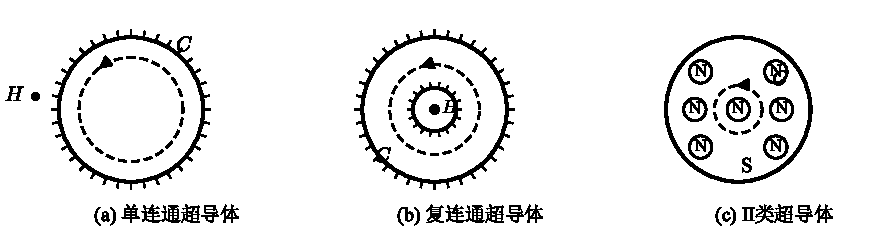
\includegraphics[width=9.5cm]{fig6-18.pdf}\\[0.3em]
{\small (a) 单连通超导体\qquad (b) 复连通超导体\qquad (c) Ⅱ类超导体}\\[0.2em]
{\small 图 6.18}
\end{minipage}
\end{center}

\begin{equation}
  \Delta(\boldsymbol{r})=V\langle\Psi_{\downarrow}(\boldsymbol{r})
  \Psi_{\uparrow}(\boldsymbol{r})\rangle
\end{equation}
将上式中场量 $\Psi_{\sigma}(\boldsymbol{r})$ 用平面波展开，对于空间均匀情形，利用平移不变性，仍可以求得超导的能隙函数与位置无关.一般情况下，$\Delta(\boldsymbol{r})$ 显然是一个与位置 $\boldsymbol{r}$ 有关的复量，$\Delta(\boldsymbol{r})$ 相当于G-L的复有序参量 $\psi(\boldsymbol{r})$.戈尔柯夫（Gorkov）用格林函数方法首先证明了 $\Delta(\boldsymbol{r})$ 所满足的方程与G-L方程相同，G-L的序参量 $\psi(\boldsymbol{r})$ 与能隙函数成正比\textsuperscript{[10]}
\begin{equation}
  \psi(\boldsymbol{r})=\frac{\left[7\zeta(3)\,n\right]^{1/2}}
  {4\pi k_{\mathrm{B}}T_{\mathrm{c}}}\,\Delta(\boldsymbol{r})
\end{equation}
并有对应关系 $e^{*}=2e$ 和 $m^{*}=2m$，进一步证实了G-L序参量代表超导体中库柏对的形成.此外，G-L方程中的唯象参数 $\alpha$、$\beta$、$\lambda(T)$、$\xi(T)$ 都能从微观理论求出.对于纯样品有\textsuperscript{[10]}
\begin{equation}
  \alpha=1.83\,\frac{\hbar^{2}}{2m}\frac{1}{\xi_{0}}
  \frac{T-T_{\mathrm{c}}}{T_{\mathrm{c}}}
  \qquad\left(T<T_{\mathrm{c}}\right)
\end{equation}
\begin{equation}
  \beta=0.35\,\frac{1}{g(0)}
  \left(\frac{\hbar^{2}}{2m}\frac{1}{\xi_{0}}\right)^{2}
  \frac{1}{\left(k_{\mathrm{B}}T_{\mathrm{c}}\right)^{2}}
\end{equation}
\begin{equation}
  \lambda(T)=\frac{1}{\sqrt{2}}\lambda_{\mathrm{L}}(0)
  \left(\frac{T_{\mathrm{c}}}{T_{\mathrm{c}}-T}\right)^{1/2}
\end{equation}
\begin{equation}
  \xi(T)=0.74\left(\frac{T_{\mathrm{c}}}{T_{\mathrm{c}}-T}\right)^{1/2}\xi_{0}
\end{equation}
其中费密面上的态密度 $g(0)$、伦敦穿透深度 $\lambda_{\mathrm{L}}(0)$ 及BCS相干长度 $\xi_{0}$ 等在微观理论中均为已知量.

从式(6.10.34)可知，$\psi(\boldsymbol{r})\sim
\langle\Psi_{\downarrow}(\boldsymbol{r})\Psi_{\uparrow}(\boldsymbol{r})\rangle$，若将G-L波函数 $\psi(\boldsymbol{r})$ 写成
\begin{equation}
  \psi(\boldsymbol{r})=\sqrt{n_{\mathrm{s}}(\boldsymbol{r})}\,
  \mathrm{e}^{\mathrm{i}\varphi(\boldsymbol{r})}
\end{equation}
则其中的相位 $\varphi(\boldsymbol{r})$ 就是
$\langle\Psi_{\downarrow}(\boldsymbol{r})\Psi_{\uparrow}(\boldsymbol{r})\rangle$
的相位，物理上代表在产生或消灭一个电子对的那些状态上的概率幅的相对相位.在空间均匀情况下，$\varphi(\boldsymbol{r})=\varphi$ 正好代表BCS基态波函数中 $\left(u_{k}/v_{k}\right)$ 的相位 $\varphi$，如式(6.9.13)所表示.简言之，G-L宏观波函数 $\psi(\boldsymbol{r})$ 的相位就是能隙函数 $\Delta(\boldsymbol{r})$ 的相位.因此，在空间均匀情况下，一个孤立的大块超导样品的G-L波函数可表示为
\begin{equation}
  \psi=\sqrt{n_{\mathrm{s}}}\,\mathrm{e}^{\mathrm{i}\varphi}
\end{equation}
其中 $|\psi|^{2}=n_{\mathrm{s}}$ 代表参与配对凝聚的超导电子浓度，而其常数相位 $\varphi$ 则表明所有参加库柏对凝聚的超导电子都具有相同的相位，此即相位相干，正是这种相位相干的库柏对传输超电流.在这个意义上，人们常说G-L波函数 $\psi$ 是描述BCS超导体中所有库柏对的一个宏观波函数.

\subsection*{5. 约瑟夫森效应}

1962年，一个年轻的英国物理学研究生约瑟夫森（Josephson）\textsuperscript{[13]}在分析了超导体中相位相干及其随时间的演化特征后，提出了两项理论预言.

（i）若用一块足够薄的绝缘层（厚度d约为1～2nm）将两块超导体1与2隔开，形成隧道结，则有可能观测到由于库柏对隧穿的无阻超电流
\begin{equation}
  I=I_{0}\sin\gamma
  \qquad\left(\gamma=\varphi_{2}-\varphi_{1}\right)
\end{equation}
其中 $\gamma=\varphi_{2}-\varphi_{1}$ 代表两块超导体间的相位差，这就是直流约瑟夫森效应.

（ii）若在隧道结两端施加一个恒定的电压 $V_{0}$，则隧穿电流将按频率 $\omega_{0}=\left(2eV_{0}/\hbar\right)$ 随时间t变化，形成交流隧穿
\begin{equation}
  I(t)=I_{0}\sin\left(\omega_{0}t+\gamma_{0}\right)
  \qquad\left(\omega_{0}=2eV_{0}/\hbar\right)
\end{equation}
被称为交流约瑟夫森效应.这是两项惊人的预言，不久即为实验所证实，并由此带动了包括超导磁强计在内的一系列超导电子器件的迅猛发展.

利用G-L方程也可以导出约瑟夫森效应的两个基本公式(6.10.41)和式(6.10.42)，首先讨论无外场 $\left(\boldsymbol{A}=0\right)$ 时的直流约瑟夫森效应.

直流约瑟夫森效应：当 $\boldsymbol{A}=0$ 时，根据G-L方程式(6.10.11)在超导体1中沿z方向的电流密度为
\begin{equation}
  j_{z}=-\left(\frac{\mathrm{i}\hbar e^{*}}{2m^{*}}\right)
  \left(\psi^{*}_{1}\frac{\partial\psi_{1}}{\partial z}
  -\psi_{1}\frac{\partial\psi^{*}_{1}}{\partial z}\right)\equiv j_{\mathrm{s}}
\end{equation}
当氧化层的厚度 $d\gg\xi$（相干长度）时，根据G-L边界条件式(6.10.9)有
\begin{equation*}
  -\mathrm{i}\hbar\,\frac{\partial\psi_{1}}{\partial z}(\boldsymbol{r})=0
\end{equation*}
表示无电流隧穿结区.对于约瑟夫森隧道结，由于氧化层的厚度d只有1～2nm，自然属于相反的情形 $d\ll\xi$，这时
$\psi_{1}=|\psi_{1}|\,\mathrm{e}^{\mathrm{i}\varphi_{1}}$ 与
$\psi_{2}=|\psi_{2}|\,\mathrm{e}^{\mathrm{i}\varphi_{2}}$
均可以部分地透入对方，导致在结区附近两者有一定的关系，通常可以用一个唯象的"边界"条件表示为
\begin{equation}
  -\mathrm{i}\hbar\,\frac{\partial\psi_{1}}{\partial z}
  =-\mathrm{i}\,\frac{\hbar}{b}\psi_{2}
\end{equation}
其中b具有长度量纲，于是将有电流隧穿结区.这个唯象条件在物理上对应于有电子对运动所产生的超电流 $\left(\sim\partial\psi_{1}/\partial z\right)$ 从超导体1向超导体2中转移，从而成为超导体2中的凝聚对，并用 $\psi_{2}$ 描述.

将式(6.10.44)代入式(6.10.43)求得
\begin{equation*}
\begin{aligned}
  j_{\mathrm{s}}
  &=-\mathrm{i}\left(\frac{e^{*}\hbar}{m^{*}b}\right)\frac{1}{2}
  \left(\psi^{*}_{1}\psi_{2}-\psi_{1}\psi^{*}_{2}\right)\\
  &=\left(\frac{e^{*}\hbar}{m^{*}b}\right)
  |\psi_{1}|\,|\psi_{2}|\sin\left(\varphi_{2}-\varphi_{1}\right)
\end{aligned}
\end{equation*}
因此
\begin{equation}
  j_{\mathrm{s}}=j_{0}\sin\gamma
  \qquad\left(\gamma=\varphi_{2}-\varphi_{1}\right)
\end{equation}
其中 $j_{0}\equiv\left(e^{*}\hbar/m^{*}b\right)|\psi_{1}|\,|\psi_{2}|$，上式乘以结区面积即为直流约瑟夫森效应公式(6.10.41).

为了讨论在外场（包括电场 $\boldsymbol{E}$ 和磁场 $\boldsymbol{B}$）中的约瑟夫森效应，还必须引进具有规范不变性的相位差，以保证可观测量如电流密度j等不受规范变换的影响.当存在外场A时，根据G-L方程式(6.10.11)，并考虑到 $\psi=|\psi|\,\mathrm{e}^{\mathrm{i}\varphi}$ 及 $|\psi|^{2}=n_{\mathrm{s}}$，可得超电流密度
\begin{equation}
\begin{aligned}
  \boldsymbol{j}_{\mathrm{s}}
  &=-\mathrm{i}\left(\frac{e^{*}\hbar}{2m^{*}}\right)
  \left(\psi^{*}\nabla\psi-\psi\nabla\psi^{*}\right)
  -\frac{\left(e^{*}\right)^{2}}{m^{*}c}|\psi|^{2}\boldsymbol{A}\\
  &=\frac{n_{\mathrm{s}}e^{*}}{m^{*}}
  \left(\hbar\nabla\varphi-\frac{e^{*}}{c}\boldsymbol{A}\right)
  \equiv\frac{n_{\mathrm{s}}e^{*}}{m^{*}}\boldsymbol{v}_{\mathrm{s}}
\end{aligned}
\end{equation}
其中 $e^{*}=2e$ 和 $m^{*}=2m$，物理上对应于库柏对传输超电流，而超电流的速度为
\begin{equation}
  \boldsymbol{v}_{\mathrm{s}}
  =\left(\hbar\nabla\varphi-\frac{e^{*}}{c}\boldsymbol{A}\right)
\end{equation}
由于 $\boldsymbol{v}_{\mathrm{s}}$ 是可观测的物理量，它应具有规范不变性.换句话说，当我们对矢量势A作规范变换
$\boldsymbol{A}\to\boldsymbol{A}'+\nabla\chi$ 时，相位 $\varphi$ 必须要有相应的改变
$\varphi\to\varphi'+\dfrac{e^{*}}{\hbar c}\chi$
才能保持 $\boldsymbol{v}_{\mathrm{s}}$ 不变.由此可知，在上述直流约瑟夫森效应的电流公式中 $\left(\varphi_{2}-\varphi_{1}\right)$ 不具有规范不变性.为了使 $j_{z}$ 也保持规范不变性，我们必须改用下列规范不变的相位差
\begin{equation}
  \gamma=\varphi_{2}-\varphi_{1}
  -\frac{e^{*}}{\hbar c}\int_{1}^{2}A_{z}\,\mathrm{d}z
\end{equation}
用于讨论磁场效应.考虑两个半无限的超导体1与2被一个沿z方向厚度为d的氧化层所隔开，磁场 $B_{0}$ 沿y轴，这时可取矢量势为
\begin{equation*}
  A_{x}=0\text{，}\qquad A_{y}=0\text{，}\qquad A_{z}=A_{z}(x)
\end{equation*}
和
\begin{equation*}
  B_{y}(x)=-\frac{\partial A_{z}}{\partial x}=B_{0}
\end{equation*}
在此情况下，规范不变的相位差式(6.10.48)随x变化，可写为
\begin{equation*}
\begin{aligned}
  \gamma(x)&=\gamma(0)-\frac{2e}{\hbar c}
  \int_{-\frac{d}{2}-\lambda}^{\frac{d}{2}+\lambda}
  A_{z}(x)\,\mathrm{d}z\\
  &=\gamma(0)-\frac{2e}{\hbar c}A_{z}(x)\left(d+2\lambda\right)
\end{aligned}
\end{equation*}
其中 $\gamma(0)\equiv\varphi_{2}-\varphi_{1}$.此外，还考虑了磁场 $B_{y}(x)$ 在1与2中各有 $\lambda$ 的磁场穿透深度.在恒定磁场情形
\begin{equation*}
  B_{y}(x)=B_{0}\text{，}\qquad A_{z}(x)=-B_{0}x
\end{equation*}
这时磁场的存在将导致结中相位差的空间变化（空间调制）
\begin{equation*}
  \gamma(x)=\gamma(0)+\frac{2e}{\hbar c}B_{0}\left(d+2\lambda\right)x
\end{equation*}
根据约瑟夫森关系式(6.10.45)，相位的空间调制又将使x点的电流密度被调制为
\begin{equation*}
  j_{\mathrm{s}}(x)=j_{0}\sin\gamma(x)
  =j_{0}\sin\left[\gamma(0)
  +\frac{2e}{\hbar c}B_{0}\left(d+2\lambda\right)x\right]
\end{equation*}
对于沿x方向尺度为D和y方向长度为L的结，流过总面积为LD，隧道结的超电流为
\begin{equation}
\begin{aligned}
  I_{\mathrm{s}}&=L\int_{-D/2}^{D/2}\mathrm{d}x\,j_{\mathrm{s}}(x)\\
  &=Lj_{0}\int_{-D/2}^{D/2}\mathrm{d}x\left\{\sin\gamma(0)
  \cos\left[\frac{2e}{\hbar c}B_{0}\left(d+2\lambda\right)x\right]\right.\\
  &\quad\left.+\cos\gamma(0)
  \sin\left[\frac{2e}{\hbar c}B_{0}\left(d+2\lambda\right)x\right]\right\}\\
  &=j_{0}LD\,\frac{\sin\left(\pi\Phi/\Phi_{0}\right)}
  {\left(\pi\Phi/\Phi_{0}\right)}\sin\left(\varphi_{2}-\varphi_{1}\right)
\end{aligned}
\end{equation}
其中穿过结区的总磁通量为 $\Phi=B_{0}\left[\left(d+2\lambda\right)D\right]$，这里方括号内的量代表y方向磁场的穿透面积，而
$\Phi_{0}=\left(\pi\hbar c/e\right)=2.07\times10^{-7}\,\mathrm{Gs\cdot cm^{2}}$
为磁通量子.这时通过隧道结的超电流（即零电压电流）的最大值作为磁场的函数可表示为
\begin{equation}
  I_{\max}=I_{0}\left|\frac{\sin\left(\pi\Phi/\Phi_{0}\right)}
  {\left(\pi\Phi/\Phi_{0}\right)}\right|
  \qquad\left(I_{0}\equiv j_{0}LD\right)
\end{equation}
上式表明通过结的超电流最大值对磁场很敏感，当穿过结的通量改变一个磁通量子时，$I_{\max}$ 将从中心的极大值 $I_{0}$ 下降到零，然后随着磁场的增大 $I_{\max}$ 又回复到较小的极大并依次重复，如图6.19所示，呈现出与光学中单缝衍射图相似的形状，在物理上代表磁场对相位的空间调制所产生的宏观量子衍射现象.这个理论结果与1963年安德逊与罗威尔（Rowell）\textsuperscript{[14]}在
$\mathrm{Sn-SnO-Sn}$ 隧道结中的测量结果几乎是惊人地一致，从而令人信服地证实了直流J效应的存在.很容易想到，可以利用 $I_{\mathrm{c}}$ 随 $\Phi/\Phi_{0}$ 的周期性起伏来测量磁场.但是，由于磁场穿透结区的面积很小［大致为
$\left(1\sim2\right)\times10^{-7}\,\mathrm{cm^{2}}$］，相邻两电流峰值（即一个 $\Phi_{0}$）所对应的磁场改变仅为1Gs量级，即使设法能准确测量到电流起伏周期的百分之一，也不过达到0.01Gs的灵敏度.所以，要利用这种效应作高敏度的磁场测量，还需另想办法，我们将在本节最后部分介绍双结干涉效应时再作讨论.

\begin{center}
\begin{minipage}{6.5cm}
\centering
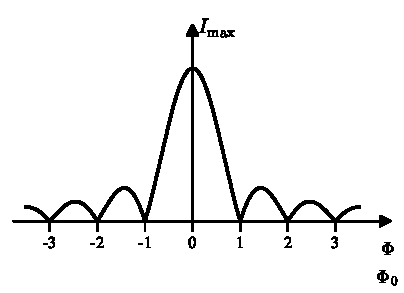
\includegraphics[width=6.5cm]{fig6-19.pdf}\\{\small 图 6.19\quad 通过约瑟夫森结的超电流最大值与磁通量之间的关系}
\end{minipage}
\end{center}

交流约瑟夫森效应：利用规范不变的相位差公式(6.10.48)还可以导出交流约瑟夫森效应.设沿z方向存在电场 $E_{z}$，根据电动力学
$E_{z}=-\dfrac{1}{c}\left(\dfrac{\partial A_{z}}{\partial t}\right)$，
矢量势 $A_{z}$ 应随时间t变化，这时对式(6.10.48)求时间导数，得到
\begin{equation}
  \frac{\partial\gamma}{\partial t}
  =-\frac{2e}{\hbar c}\int_{1}^{2}\frac{\partial A_{z}}{\partial t}\,\mathrm{d}z
  =\frac{2e}{\hbar}\int_{1}^{2}E_{z}\,\mathrm{d}z
  =\frac{2eV}{\hbar}
\end{equation}
其中V代表结区的电压.当V为常量电压 $V_{0}$ 时，$\gamma$ 是时间t的线性函数
$\gamma=\left(2eV_{0}/\hbar\right)t+\gamma_{0}$，
其中 $\gamma_{0}$ 代表1与2两块超导体间的初始相位差，因此约瑟夫森电流密度为
\begin{equation}
  j_{z}=j_{0}\sin\gamma=j_{0}\sin\left(\omega_{0}t+\gamma_{0}\right)
\end{equation}
其中
\begin{equation}
  \omega_{0}=\frac{2eV_{0}}{\hbar}
\end{equation}
上式表明，当两块超导体间存在恒定电压 $V_{0}$ 时，将产生频率为 $\omega_{0}$ 的交变电流，这时式(6.10.52)乘以隧道结的截面积LD就得到式(6.10.42)，此即著名的交流约瑟夫森效应.当外加压 $V_{0}=10\ \mu\mathrm{V}$ 时，交流约瑟夫森电流的频率为
$\omega_{0}=483.6\times10^{7}\,\mathrm{Hz}$，
恰好落在微波频率范围.人们自然会想到，如果用频率为 $\omega$ 的微波辐射照射处于直流偏压 $V_{0}$ 的约瑟夫森结将会出现反映交流约瑟夫森效应特征的新现象.事实上，约瑟夫森本人在预言交流约瑟夫森效应时就提出了这个设想，并建议以此作为验证交流约瑟夫森效应的实验手段.这时在隧道结两端的电压为
\begin{equation}
  V(t)=V_{0}+v_{0}\cos\omega t
\end{equation}
其中 $v_{0}\cos\omega t$ 是附加微波交变电压，而 $\omega$ 是微波频率，将上式代入式(6.10.51)，积分后可求出结两边超导体的电流相位差
\begin{equation}
  \gamma(t)=\frac{2e}{\hbar}V_{0}t+\gamma_{0}
  +\frac{2ev_{0}}{\hbar\omega}\sin\omega t
\end{equation}
和相应的超电流密度
\begin{equation}
  j_{\mathrm{s}}(t)=j_{0}\sin\left[\left(\frac{2e}{\hbar}V_{0}t+\gamma_{0}\right)
  +\left(\frac{2ev_{0}}{\hbar\omega}\right)\sin\omega t\right]
\end{equation}
再利用熟知的数学公式
\begin{equation*}
  \cos\left(a\sin x\right)=\sum_{m=-\infty}^{\infty}\mathrm{J}_{m}(a)\cos mx\text{，}
  \qquad
  \sin\left(a\sin x\right)=\sum_{m=-\infty}^{\infty}\mathrm{J}_{m}(a)\sin mx
\end{equation*}
又得到一个有用的公式
\begin{equation}
  \sin\left(b+a\sin x\right)
  =\sum_{m=-\infty}^{\infty}\mathrm{J}_{m}(a)\sin\left(b+mx\right)
\end{equation}
其中 $\mathrm{J}_{m}$ 代表m阶柱贝塞尔（Bessel）函数.若取 $a=\left(\dfrac{2ev_{0}}{\hbar\omega}\right)$、
$b=\left(2e/\hbar\right)V_{0}t+\gamma_{0}$ 和 $x=\omega t$，则式(6.10.56)可表示为
\begin{equation}
  j_{\mathrm{s}}(t)=j_{0}\sum_{m=-\infty}^{\infty}
  \mathrm{J}_{m}\left(\frac{2ev_{0}}{\hbar\omega}\right)
  \sin\left[\left(\frac{2e}{\hbar}V_{0}+m\omega\right)t+\gamma_{0}\right]
\end{equation}
注意在 $V_{0}$ 取任意值时，一般说来因子
$\left(\dfrac{2e}{\hbar}V_{0}t+m\omega\right)$ 不等于零，上式中所有的项都是交变电流.但是，对于某些特定的直流偏压 $V_{0}$，当满足
\begin{equation}
  2eV_{0}=n\hbar\omega
  \qquad\left(n=0,1,2,\cdots\right)
\end{equation}
时，情况却发生了变化，此时 $j_{\mathrm{s}}$ 中将出现一组零频电流项（即不随时间变化的直流项），它们可表示为
\begin{equation}
  j^{\mathrm{DC}}_{\mathrm{s}}
  =\mathrm{j}_{0}\left(-1\right)^{n}\mathrm{J}_{n}
  \left(\frac{2ev_{0}}{\hbar\omega}\right)\sin\gamma_{0}
\end{equation}
其中利用了n为正整数时柱贝塞尔函数的
$\mathrm{J}_{-n}(\varepsilon)=\left(-1\right)^{n}\mathrm{J}_{n}(\varepsilon)$
特性.上式表明，当初始相位差 $\gamma_{0}$ 从 $\left(-\pi/2\right)$ 变到 $\left(\pi/2\right)$ 时，电压
$V_{0}=\left(n\hbar\omega/2e\right)$ 保持不变，而超电流则从
$-|I_{0}\mathrm{J}_{n}\left(2ev_{0}/\hbar\omega\right)|$ 垂直地上升到
$+|I_{0}\mathrm{J}_{n}\left(2ev_{0}/\hbar\omega\right)|$，并在 $I$-$V$ 曲线上形成一个直流的台阶，表现出如图6.20所示的台阶结构.1964年夏皮洛（Shapiro）\textsuperscript{[15]}在
$\mathrm{Al-Al_{2}O_{3}-Sn}$ 结中首先观察到了这种电流增加一定幅度，而电压却维持不变的台阶，习惯上称为夏皮洛台阶.形成夏皮洛台阶的物理原因是由于在直流偏压下约瑟夫森结所产生的交变超电流被频率相同微波（或射频）场所调制，从而产生零频率的直流超电流分量.因此，在实验上观测到夏皮洛台阶就表明交流约瑟夫森效应已被证实.

\begin{center}
\begin{minipage}{7cm}
\centering
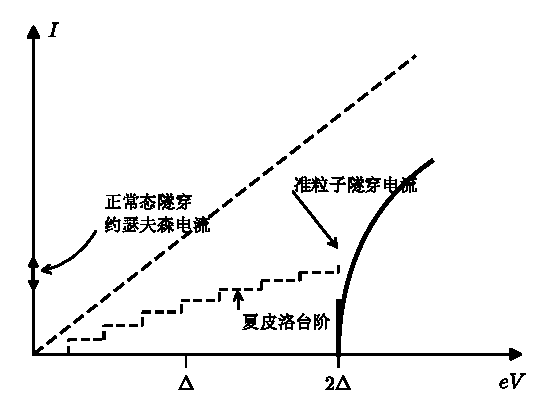
\includegraphics[width=7cm]{fig6-20.pdf}\\{\small 图 6.20\quad $I$-$V$ 曲线中夏皮洛台阶的示意图}
\end{minipage}
\end{center}

由于在第n个台阶处的电压与微波频率严格地满足
$n\omega=\left(2e/\hbar\right)V_{n}$ 关系，因此精确测定微波频率和电流阶跃处的电压可以用来精确地测定物理学中的普适常数 $\left(2e/\hbar\right)$.在20世纪60年代末期，利用交流约瑟夫森效应测出了 $\left(2e/\hbar\right)$ 的精确值，并推算出精细结构常数
$\alpha=\left(e^{2}/\hbar c\right)$，
从而解决了氢原子的超精细能级分裂的实验测量与量子电动力学理论之间的矛盾.此外，由关系式 $V_{n}=n\omega\left(\hbar/2e\right)$ 还可得知，只要选定一个台阶的号码，就可以通过测量频率 $\omega$ 而计算出台阶的电压，又由于微波频率可以精确测量到 $10^{-9}$ 甚至更高的精度，所以通过测定频率来测量电压可以达到很高的精确度.目前，利用这一方法所制成的超导电压基准已被广泛采用.

直流约瑟夫森效应的最重要应用是制作超导量子干涉仪（superconducting quantum interference devices，简称SQUID），这种仪器可用作探查或测量极其微弱的磁场.最简单的SQUID是由两个约瑟夫森结并联组成的环结构，如图6.21.为简单起见，设两个结具有相同的临界超电流 $I_{\mathrm{s}}$，外磁场垂直于环路平面，由于垂直磁场的结区面积比超导环的面积小得多，可略去透过结区的磁通，将超导环所包围的磁通量 $\Phi$ 表示为
\begin{equation}
  \Phi=\int_{S}\boldsymbol{B}\cdot\mathrm{d}\boldsymbol{S}
  =\oint\boldsymbol{A}\cdot\mathrm{d}\boldsymbol{l}
  =\int_{c}^{a}\boldsymbol{A}\cdot\mathrm{d}\boldsymbol{l}
  +\int_{b}^{d}\boldsymbol{A}\cdot\mathrm{d}\boldsymbol{l}
\end{equation}

\begin{center}
\begin{minipage}{7cm}
\centering
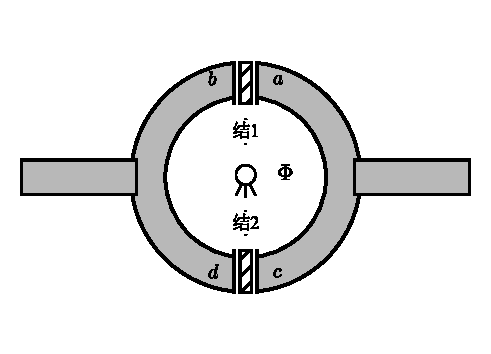
\includegraphics[width=7cm]{fig6-21.pdf}\\{\small 图 6.21\quad 双结超导干涉仪示意图}
\end{minipage}
\end{center}

而通过环的总超电流应等于通过两个结的直流约瑟夫森电流之和
\begin{equation}
  I=I_{\mathrm{J}}\left[\sin\left(\varphi_{a}-\varphi_{b}\right)
  +\sin\left(\varphi_{c}-\varphi_{d}\right)\right]
\end{equation}
其中 $I_{\mathrm{J}}$ 代表存在外磁场时单个约瑟夫森结中的最大超电流，由式(6.10.50)决定.当两个结不相干时，它们的相位差 $\left(\varphi_{a}-\varphi_{b}\right)$ 和
$\left(\varphi_{c}-\varphi_{d}\right)$ 是彼此独立的，并可以同时调节到 $\left(\pi/2\right)$，使最大的I值为 $2I_{\mathrm{J}}$，这时只有单结的衍射效应，而没有双结干涉效应.实际上a与c（或b与d）之间是超导连接，这时两个结的相位差不再是独立的，而是在 $\varphi_{a}$ 与 $\varphi_{c}$ $\left(\varphi_{b}\right.$ 与 $\left.\varphi_{d}\right)$ 之间存在着一定的约束关系，考虑到a与c是同一超导体内的两点，这两点间的相位差应满足式(6.10.46)，当超导环的横截面线度 $L\gg\lambda$（磁场的穿透深度）时，可将超导体内迈斯纳态的电流密度 $j_{\mathrm{s}}$ 取为零，这时有
\begin{equation}
  \nabla\varphi=\left(2e/\hbar c\right)\boldsymbol{A}
\end{equation}
对上式作路积分后可得
\begin{equation}
  \left.
  \begin{aligned}
    \varphi_{a}-\varphi_{c}
    &=\left(2e/\hbar c\right)\int_{c}^{a}\boldsymbol{A}\cdot\mathrm{d}\boldsymbol{l}\\
    \varphi_{b}-\varphi_{d}
    &=\left(2e/\hbar c\right)\int_{d}^{b}\boldsymbol{A}\cdot\mathrm{d}\boldsymbol{l}
  \end{aligned}\right\}
\end{equation}
从而求出结1与结2相位差之间的约束关系
\begin{equation}
\begin{aligned}
  \left(\varphi_{a}-\varphi_{b}\right)-\left(\varphi_{c}-\varphi_{d}\right)
  &=\left(\varphi_{a}-\varphi_{c}\right)+\left(\varphi_{d}-\varphi_{b}\right)\\
  &=\left(2e/\hbar c\right)\left(\int_{c}^{a}+\int_{b}^{d}\right)
  \boldsymbol{A}\cdot\mathrm{d}\boldsymbol{l}\\
  &=\left(2e/\hbar c\right)\Phi=2\pi\left(\Phi/\Phi_{0}\right)
\end{aligned}
\end{equation}
其中利用了式(6.10.61)和磁通量子 $\Phi_{0}=\left(\pi\hbar c/e\right)$.这时最好将式(6.10.62)变换为正、余弦函数之乘积，并利用约束关系式(6.10.65)求出
\begin{equation}
\begin{aligned}
  I&=2I_{\mathrm{J}}\cos\left[\frac{1}{2}
  \left(\varphi_{a}-\varphi_{c}+\varphi_{d}-\varphi_{b}\right)\right]
  \sin\left[\frac{1}{2}
  \left(\varphi_{a}+\varphi_{c}-\varphi_{d}-\varphi_{b}\right)\right]\\
  &=2I_{\mathrm{J}}\cos\left(\pi\Phi/\Phi_{0}\right)\sin\gamma_{0}
\end{aligned}
\end{equation}
其中
\begin{equation*}
  \gamma_{0}\equiv\frac{1}{2}
  \left(\varphi_{a}+\varphi_{c}-\varphi_{d}-\varphi_{b}\right)
  =\frac{1}{2}\left[\left(\varphi_{a}-\varphi_{b}\right)
  +\left(\varphi_{c}-\varphi_{d}\right)\right]
\end{equation*}
代表两个结的相位差之和，它可以任意调节，当 $\gamma_{0}=\pi/2$ 时，双结系统的超电流最大值为
\begin{equation}
  I_{\max}=2I_{\mathrm{J}}\left|\cos\left(\pi\Phi/\Phi_{0}\right)\right|
\end{equation}

\begin{center}
\begin{minipage}{7cm}
\centering
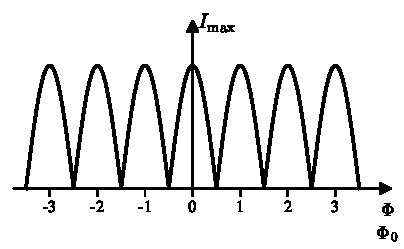
\includegraphics[width=7cm]{fig6-22.pdf}\\{\small 图 6.22\quad 双结超导环的干涉效应}
\end{minipage}
\end{center}

图6.22是以 $I_{\mathrm{J}}$ 为单位、$I_{\max}$ 随 $\left(\pi\Phi/\Phi_{0}\right)$ 的变化曲线.显然，当环路所包含的 $\Phi$ 为 $\Phi_{0}$ 的整数倍时，给出 $I_{\max}$ 之极大值，而当 $\left(\Phi/\Phi_{0}\right)$ 为半整数时 $I_{\max}$ 降为零，它至少可以区别半个磁通量子
$\Phi_{0}=2\times10^{-7}\,\mathrm{Gs\cdot cm^{2}}$ 的变化，这就是双结干涉效应.由于超导环路所包围的面积S是可以人为控制的，人们只需制作面积的数量级为 $1\ \mathrm{cm^{2}}$ 的双结超导环，就可以探测到 $10^{-7}\,\mathrm{Gs}$ 的磁场变化.因此，双结干涉效应可用于制作高精度的磁场测量仪——磁强计.

在以上的讨论中，我们还没有考虑单结衍射效应对双结干涉效应的影响.若再将式(6.10.67)中的 $I_{\mathrm{J}}$ 用外磁场中的单结衍射公式(6.10.50)代入，则求得包括了干涉与衍射效应的双结系统的超电流最大值满足
\begin{equation}
  I_{\max}=2I_{0}\left|\frac{\sin\left(\pi\Phi_{\mathrm{J}}/\Phi_{0}\right)}
  {\left(\pi\Phi_{\mathrm{J}}/\Phi_{0}\right)}\right|
  \left|\cos\left(\pi\Phi/\Phi_{0}\right)\right|
\end{equation}
其中 $\Phi_{\mathrm{J}}$ 是结区穿透范围内的磁通量，由于超导环路所包围的面积S远远大于结区被磁场穿透的面积，在上式中，$\Phi_{\mathrm{J}}\ll\Phi$（穿过环路的总磁通量），这时上式中因子
$\left|\cos\left(\pi\Phi/\Phi_{0}\right)\right|$ 导致 $I_{\max}$ 随外磁场作小周期的快速振荡，而来自结衍射效应的
$\left|\sin\left(\pi\Phi_{\mathrm{J}}/\Phi_{0}\right)
/\left(\pi\Phi_{\mathrm{J}}/\Phi_{0}\right)\right|$
因子则随磁场作较长周期的衰减振荡，从而对小周期振荡的干涉效应起着调制作用.理论与实验结果都表明双结系统的 $I_{\max}$-$B$ 曲线如图6.23所示，它显示出受到衍射调制的干涉图样.最后，我们还要指出，仅仅根据 $I_{\max}$ 从极大变为极小（即一个干涉条件），只能测定出数量级为一个磁通量子 $\Phi_{0}$ 的磁场 $\left(10^{-7}\,\mathrm{Gs}\right)$，而当 $\Phi=\Phi_{0}$ 时，必然有 $\Phi_{\mathrm{J}}\ll\Phi_{0}$，这时式(6.10.68)退化为式(6.10.67).因此，作微小磁场测量时，主要是利用干涉效应，即式(6.10.67).目前在双结干涉效应基础上人们已制造出直流SQUID，其中利用补偿磁通（或抵消磁场）方法已能读出 $10^{-4}\Phi_{0}$ 的微小磁通变化，相当于能分辨出 $10^{-11}\,\mathrm{Gs}$ 微弱磁场变化，详细讨论可参阅文献\textsuperscript{[16]}.

\begin{center}
\begin{minipage}{7cm}
\centering
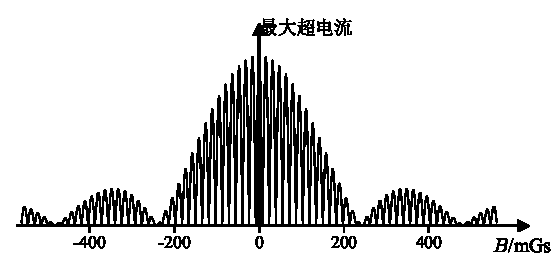
\includegraphics[width=7cm]{fig6-23.pdf}\\{\small 图 6.23\quad 双结SQUID的衍射调制干涉图样}
\end{minipage}
\end{center}

\begin{canKao}
\begin{enumerate}[label={[\arabic*]}, leftmargin=2.2em, itemsep=0pt]
\item Cooper L N. Phys Rev, 1956, 104: 1189
\item Bardeen J, Cooper L N, Schrieffer J R. Phys Rev, 1957, 103: 1175
\item Mahen G D. Many-particle Physics. New York: Plenum Press, 1981. Chap 7
\item De Gennes P G. Superconductivity of Metals and Alloys. New York: Benjamin, 1966. Chap 8
\item Schrieffer J R. Theory of Superconductivity. New York: Benjamin, 1964
\item Giaever L. Phys Rev Lett, 1960, 5: 147, 464
\item 管惟炎等. 超导电性. 北京: 科学出版社，1981. 第6章
\item Fetter A L, Walecka J D. Quantum Theory of Many-particles System. New York: Mc-Graw-Hill, 1971. Chap 13
\item Ginzburg V L, Landau L D. Zh Eksper Teor Fis, 1950, 24: 1064
\item Saint-James D et al. Type Ⅱ Superconductors. London: Pergamon Press, 1969
\item Deaver B S, Fairbank W M. Phys Rev Lett, 1961, 7: 43
\item Abrikosov A A. Zh Eksper Teor Fis, 1957, 32: 1442
\item Josephson B D. Phys Lett, 1960, 1: 251; Adv Phys, 1965, 14: 419
\item Anderson P W, Rowell J M. Phys Rev Lett, 1963, 10: 230
\item Shapiro S. Phys Rev Lett, 1963, 11: 80
\item 陈式刚等. 高温超导研究. 四川教育出版社，1991.6
\end{enumerate}
\end{canKao}
